\documentclass[12pt]{article}

\usepackage[a4paper,margin=1in]{geometry}
\usepackage{amsmath,amssymb}
\usepackage{graphicx}
\usepackage{float}
\usepackage{tabularx}
\usepackage{array}
\usepackage{longtable}
\usepackage{enumitem}
\usepackage{url}
\usepackage[colorlinks=true,linkcolor=blue,citecolor=blue,urlcolor=blue]{hyperref}
\usepackage{setspace}
\usepackage{authblk}
\usepackage{caption}

\setstretch{1.15}
\captionsetup{font=small,labelfont=bf}
\setlist[itemize]{leftmargin=1.2em}
\setlist[enumerate]{leftmargin=1.5em}
\newcolumntype{Y}{>{\raggedright\arraybackslash}X}
\newcommand{\kwh}{\mathrm{kWh}}
\newcommand{\figref}[1]{Fig.~\ref{#1}}
\newcommand{\tabref}[1]{Table~\ref{#1}}

\title{Multi-actor compliance feasibility of managed EV charging: participation constraints, a congestion-game diagnosis, and the incentive lever}
\author[1]{Peijia Pok}
\author[2]{Soomin Woo}
\author[1]{Hwasoo Yeo\thanks{Corresponding author: hwasoo@kaist.ac.kr}}
\affil[1]{Department of Civil and Environmental Engineering, KAIST, Daejeon, Republic of Korea}
\affil[2]{Department of Smart Vehicle Engineering, Konkuk University, Seoul, Republic of Korea}
\date{}

\begin{document}
\maketitle

\section*{Highlights}
\begin{itemize}
    \item Multi-actor gates test EV charging across driver, charging operator, and grid criteria.
    \item Low-deviation behavior reduces same-episode all-pass acceptability to near zero.
    \item Request-event churn, not demanded-kWh growth, explains the behavioral failure mode.
    \item A calibrated congestion-game overlay interprets the collapse as an uncoordinated compliance equilibrium.
    \item A bounded compliance incentive restores modelled all-pass acceptability across tested capacities.
\end{itemize}

\begin{abstract}
Managed electric-vehicle (EV) charging is usually optimized as a multi-objective trade-off of cost, service, and grid objectives---the right tool for an efficient \emph{average} operating point. Deployment, however, is a different question: a program runs only if drivers, charging operators, and the grid each stay above their own minimum requirement at the same time, in the actual operating period. These requirements are \emph{non-compensatory}, whereas a blended objective is compensatory and averaged---so a policy can look attractive on the blend yet fail an individual actor in specific periods, and that actor then opts out and the program stalls. We therefore treat deployability as joint \emph{feasibility}, complementary to optimization rather than replacing it: each actor's requirement is a participation constraint, an episode is feasible when all three hold together, and we measure the fraction of feasible episodes. Using a charging-demand model calibrated to public ACN-Data, we show that trade-off optimality does not imply feasibility---a lowest-cost policy in the tested set that dominates a service policy on cost and reliability still has $0\%$ feasible episodes; that feasibility has a sharp behavioral threshold, falling from $96.7\%$ under full compliance to $1.2\%$ once non-compliance exceeds about $1.5\%$ ($\sim$98.5\% recommendation adherence), a property that survives our strongest refutation tests---two recognized deadline schedulers, a best-per-episode oracle ($5\%$), and every weighting of the three objectives---within the modeled system; and that, in a calibrated congestion-game model, the operator's effective lever is not a better scheduler but a Pigouvian-style compliance incentive that restores feasibility, with a price of anarchy near $1.5$. The contribution is a participation-feasibility account of managed-charging deployment: a compliance threshold and an incentive lever established as structural properties of the model, while whether real fleets sit in the infeasible regime---an empirical question anchored to deviation magnitudes, not fitted to field opt-out---is left open.
\end{abstract}

\noindent\textbf{Keywords:} electric vehicle charging; managed charging; multi-actor acceptability; driver behavior stress testing; operator dispatch; distribution feeder; IEEE-33

\section*{Nomenclature}
\begin{longtable}{p{0.18\textwidth}p{0.76\textwidth}}
\textbf{Abbreviations} & \\
EV & Electric vehicle \\
IEEE-33 & IEEE 33-bus radial distribution benchmark \\
SoC & State of charge \\
\textbf{Sets and indices} & \\
$i \in \mathcal{I}$ & EV index \\
$t \in \mathcal{T}$ & Simulation timestep index \\
$s \in \mathcal{S}$ & Random-seed index \\
$c \in \mathcal{C}$ & Capacity-level index \\
$b \in \mathcal{B}$ & Behavior-model index \\
$f \in \mathcal{F}$ & Operator-policy index \\
$g \in \mathcal{G}$ & Grid-policy index \\
$r \in \mathcal{R}_t$ & Request event active at timestep $t$ \\
$e$ & Simulation episode, $e=(s,c,b,f,g,H)$ \\
\textbf{Decision and state variables} & \\
$x^F_{r,t}$ & Operator-recommended service action for request $r$ at timestep $t$ \\
$x^G_{r,t}$ & Grid-adjusted service action \\
$x_{r,t}$ & Final served action \\
$E^{req}_r$ & Energy represented by simulator request event $r$ (kWh) \\
$E^{dem}_{i,t}$ & Operational demanded energy used in the demanded-kWh trace (kWh) \\
$E^{rem}_{pre},E^{rem}_{post}$ & Pre-step and post-step remaining demanded energy in the ledger audit (kWh) \\
$E^{new}$ & New demanded-kWh increment in the ledger audit (kWh) \\
$E^{delivered}$ & Delivered energy credited to outstanding simulator demand (kWh) \\
$E^{release}$ & Demand reduction not explained by delivered charging, explicitly closing the ledger identity (kWh) \\
$N^{actual},N^F$ & Actual driver-layer request-event count and operator-recommended request-event count \\
$\chi$ & Actual/operator-recommended request-event ratio, $N^{actual}/N^F$ \\
$L_t$ & Site load at timestep $t$ \\
$P_t$ & Peak-pressure or price-related signal \\
\textbf{Metrics and thresholds} & \\
$A_D,A_O,A_G$ & Driver, charging operator, and grid acceptability indicators \\
$A_{all}$ & All-pass acceptability indicator \\
$\rho_E$ & Delivered-energy ratio \\
$\Delta_R$ & Reliability delta relative to anchor \\
$\eta_D$ & Driver unmet-service metric \\
$S_F$ & Charging-operator service-completion metric \\
$Q_F$ & Charging-operator queue or request-volume pressure \\
$K_F$ & Charging-operator cost or operating penalty proxy \\
$\rho_P$ & Peak ratio relative to anchor \\
$\rho_{ramp}$ & Ramp ratio relative to anchor \\
$\Delta LF$ & Load-factor change relative to anchor \\
$\tau$ & Generic actor-gate threshold \\
\end{longtable}

\section{Introduction}

Electrification of road transport is shifting a substantial share of energy demand from liquid fuels to electricity networks. At the same time, charging infrastructure is frequently installed behind local service connections, depot transformers, workplace panels, or distribution feeders whose capacity was not designed around synchronized high-power EV charging. This creates a planning and operating problem that is central to applied energy systems: charging should deliver enough energy to drivers and operator services, but it should also avoid producing grid peaks, ramps, losses, and line-loading stress that undermine local power-system operation. The problem is not only to compute a schedule that improves one metric. The practical question is whether a charging-control policy is acceptable to all relevant actors under the constraints and behaviors expected during operation.

The literature has strong foundations for coordinated and decentralized EV charging control \cite{ma2013,gan2013,sortomme2011,rotering2011,richardson2012local,lee2021adaptive,nimalsiri2020,sadeghian2022,liu2019decentralized,pournaras2019}, including multi-objective formulations exposing cost--service--grid trade-offs on a Pareto frontier \cite{wang2024multiobj,das2020technoecon}, simulation-driven evaluation \cite{lee2019acnsim,quiros2018}, grid-impact modeling \cite{lopes2011,richardson2013,shaukat2018}, facility-level cost-service analysis \cite{woo2021}, and fleet/depot coordination of capacity, generation, and storage \cite{liu2024busdepot,passow2025fleet}. A separate strand shows managed charging depends on user acceptance, trust, and convenience \cite{will2016,bailey2015,schmalfuss2015,delmonte2020,tarroja2021,sovacool2018,hardman2018,funke2019}, and that real participation, opt-out, and compliance are incentive-sensitive and only partially predictable---monetary incentives shift charge timing while non-monetary nudges often do not \cite{alexeenko2023pilot,dudek2021electricnation,bailey2025fieldexp,wong2023incentives,marxen2023flexibility}. Charging is also studied as a service-quality and fairness problem (waiting, queue delay, equitable allocation) \cite{woo2021,danner2021,tan2023fair,tsaousoglou2023fair,theodoropoulos2022proportional} and as a distribution-system stressor (feeder voltage, loading, losses, peaks) \cite{clement2010,elnozahy2014,green2011,muratori2018,dubey2015,pieltain2011,powell2022}. These strands motivate a broader evaluation stance: a policy attractive to the charging operator for serving many requests may be unacceptable to drivers on reliability; one that cuts cost or queueing may fail operator service completion; and a grid policy may improve a peak ratio while leaving driver and operator failures unresolved. Multi-criteria and social-acceptance methods are well established for energy decisions \cite{wang2009mcda,wustenhagen2007acceptance} but rarely applied to EV charging control as a same-episode, multi-actor pass/fail screen.

This paper therefore reframes the project as a question of deployment \emph{feasibility} rather than of controller superiority or objective optimization. Whether a managed-charging program can run is a multi-actor \emph{participation} problem: drivers, charging operators, and the grid each accept and keep participating only if their own minimum requirement is met, in the actual operating period, and these requirements are \emph{non-compensatory}---a low operating cost does not compensate a grid operator facing a dangerous peak, and a healthy load shape does not compensate a driver whose vehicle is not charged in time. This is why we evaluate against per-actor \emph{gates} rather than a multi-objective optimization. A weighted-sum or Pareto formulation is compensatory: it permits a surplus in one actor's objective to offset a deficit in another's, which is exactly the trade the actors would refuse. The gates are instead each actor's individual-rationality (participation) constraint, and the object of interest is the jointly-\emph{feasible set} where all three hold together. We do not claim optimization is the wrong tool in general---constrained, robust, or chance-constrained optimization could encode the same constraints---but that the primary object for deployment is this feasible set, with any optimization secondary and \emph{within} it. Because acceptability must hold in the realized operating period rather than on average, we measure the \emph{fraction} of episodes in which all participation constraints hold jointly. We report this as the \emph{all-pass rate}: the empirical share of feasible episodes across our factorial design (seeds, charger capacities, operator policies, and grid settings). It should be read as a design-conditional deployability rate rather than a probability over a specified real-world distribution of conditions; it plays the role of a chance-constraint measure---the share of operating periods that clear every actor's requirement at once---and our central question is whether behavioral compliance keeps it high.

We state this as a falsifiable hypothesis in two separable parts, and we are explicit throughout about which part each result speaks to. \textbf{H1 (structural).} Under the behavioral model of Section~\ref{sec:design}, per-episode joint feasibility has a compliance threshold below which the all-pass rate falls to near zero, and this threshold is (i)~invariant to the scheduling rule and (ii)~not recoverable by any weighting of the driver, operator, and grid objectives. H1 is a claim about the model, and it is deliberately \emph{refutable}: it would be false if some scheduler---even a hindsight-optimal one---or some objective weighting restored feasibility at the modeled deviation. We therefore treat the scheduler and optimizer comparisons below (Sections~\ref{sec:published} and~\ref{sec:results}) not as confirmations but as genuine attempts to \emph{break} H1, and report that it survives them. \textbf{H2 (empirical).} Real managed-charging populations operate in the compliance regime that H1 marks infeasible. H2 is the decision-relevant claim, and we do \emph{not} settle it here: our behavioral response is anchored to observed deviation \emph{magnitudes} but is not fitted to field opt-out decisions, so H1's within-model certainty does not transfer to H2. Keeping the two apart separates the structural result we establish from the empirical question a calibration study must answer, and stops the former from being read as the latter.

This paper contributes to the literature by: (1) formalizing managed-charging deployability as multi-actor compliance feasibility---per-actor participation constraints whose joint, same-episode satisfaction defines a feasible set, measured by the empirical all-pass rate across a factorial design---and motivating why this, rather than multi-objective optimization, is the primary object; (2) demonstrating concretely that trade-off optimality does not imply feasibility (a lowest-cost policy in the tested set that dominates a service policy on cost and reliability lies entirely outside the feasible set), together with a request-pipeline audit showing the failure is request-event churn rather than demanded-kWh growth; (3) identifying a sharp \emph{compliance threshold} on the feasible set ($\sim$98.5\% recommendation adherence) that holds under two recognized deadline-driven schedulers (least-laxity and earliest-deadline), establishing it as a property of behavior rather than of one scheduling rule; and (4) framing compliance as an aggregative game with a congestion externality whose no-incentive equilibrium coincides with the infeasible region, and analysing a Stackelberg compliance incentive---the operator's effective lever, rather than a better scheduler---that moves the equilibrium back into the feasible set, quantified by a relative price of anarchy; and (5) showing that the framework's \emph{diagnostic} value is portable across the two tested charging ecologies---applied to a data-grounded apartment (multi-unit-dwelling) scenario, the same-episode collapse persists but the binding actor shifts from driver service (workplace) to shared-charger capacity (apartment), and the apartment grid benefit is itself compliance-contingent. Throughout, we index non-compliance by a behavior \emph{severity} level on a $0$--$3$ scale: severity~0 is full compliance (drivers follow every recommendation), and severities~1, 2, and 3 correspond to roughly $5\%$, $20\%$, and $45\%$ vehicle-timestep deviation from the recommended action, with progressively stronger recommendation-override preferences (defined precisely in Section~\ref{sec:design}, Table~\ref{tab:severityparams}). These are transparent model-assumed stress levels calibrated to ACN deviation \emph{magnitudes}, not calibrated forecasts of real opt-out; the headline result already triggers at the mildest non-trivial level, severity~1. The incentive mechanism is likewise a Pigouvian-style design over a soft-calibrated behavioral model, not a fitted opt-out predictor.

The broader implication is not that one controller is universally best. Managed charging programs and fleet charging controllers often assume high compliance and evaluate energy, cost, or peak metrics separately. In the tested scenarios, small behavioral deviations create request-event churn---a rise in the frequency of charging-request interactions with the dispatch pipeline \emph{without} a rise in total energy demanded---and cause actor gates to fail even when energy delivery remains high. This suggests that energy-system evaluation should include explicit stakeholder gates and request-pipeline audits when assessing whether a charging-control policy is ready for deployment.

The remainder of the paper is organized as follows. Section~\ref{sec:system} describes the system context and actors. Section~\ref{sec:formulation} presents the acceptability-gate formulation and policy families. Section~\ref{sec:design} gives the experimental design and audit protocol. Section~\ref{sec:data} describes the data and simulation setup. Section~\ref{sec:results} reports the main results. Section~\ref{sec:game} develops the calibrated game-theoretic mechanism analysis. Section~\ref{sec:discussion} discusses implications. Section~\ref{sec:limitations} states limitations. Section~\ref{sec:conclusions} concludes.

\section{System context and problem setting}\label{sec:system}

The modeled system is a capacity-constrained EV charging facility or fleet-charging site with three decision layers. The driver layer generates charging request events and may deviate from recommendations according to a behavior model. The charging operator layer selects which requests to prioritize under finite capacity. The grid layer may apply a PeakPenalty intervention that defers selected charging events when the site is exposed to peak pressure. The final service layer records delivered energy, reliability, deferrals, unserved events, and load-shape outcomes.

The stakeholders are: drivers, who require adequate charging service and reliability; the \emph{charging operator}---the coordination layer at a workplace, depot, or apartment site that receives multiple charging requests, prioritizes service, allocates charging power under finite site capacity, and manages queues (we use ``charging operator'' rather than ``fleet operator'' to avoid implying vehicle ownership; it may be a facility, site, or charge-point operator)---who needs service completion, operational stability, and manageable request volume; and the grid or distribution operator, who is concerned with peak ratios, ramping, load factor, line loading, losses, and feeder stress. These actors need not agree on a single objective. For example, increasing service can increase peak demand, while deferring charging for peak management can reduce driver or operator acceptability.

\figref{fig:framework} shows the system framework. Driver behavior produces actual request events. An operator policy converts candidate events into recommended actions under charger capacity. A grid policy can adjust the recommended actions. The final charging service is evaluated against driver, charging operator, and grid gates. All-pass acceptability is the logical conjunction of those three pass indicators.

\paragraph{What is centralized and what is decentralized here.} In this study, ``decentralized'' means the actors have \emph{separate goals, information, and decision rights}---not that each vehicle runs its own charging optimization. The charging operator \emph{centrally} computes the charging recommendations under the site's capacity limit; the grid supplies an operating limit, price, or peak-management signal; and drivers keep local authority to accept, override, or opt out based on their own needs. The system is therefore \emph{hierarchically coordinated and partially decentralized}: the scheduling is centralized, while participation and the charging that actually happens are decentralized. We do \emph{not} claim a distributed algorithm in which each vehicle computes its own plan from local information (as in \cite{ma2013,gan2013,liu2019decentralized}).

\paragraph{Order in which the actors act.} The actors act in sequence: the grid issues a capacity or price signal; the operator turns the drivers' requests into individual recommendations under that signal and the site limit; each driver then follows, overrides, or opts out; and the charging that results---after this response---is what the gates score. Two driver decisions are distinct and enter at different points: the \emph{reported need} (energy, deadline, state of charge) that the operator schedules against, and the \emph{response} (follow or override) to the resulting recommendation. Non-compliance therefore enters \emph{after} the grid-adjusted recommendation. Writing $x^{G}_{r,t}$ for the grid-adjusted recommended action of request $r$ at time $t$, the action that actually happens is
\begin{equation}
x^{\mathrm{real}}_{r,t}=\pi_D\!\left(x^{G}_{r,t},\,z_{i,t},\,\theta_i,\,p_i\right),
\label{eq:driverresponse}
\end{equation}
where the driver's response rule $\pi_D$ depends on their private state $z_{i,t}$, their threshold $\theta_i$, and any incentive $p_i$; all fourteen gates are then evaluated on this realized $x^{\mathrm{real}}$, not on the recommendation. This makes explicit where behavioral non-compliance enters the pipeline.

\begin{figure}[t]
\centering
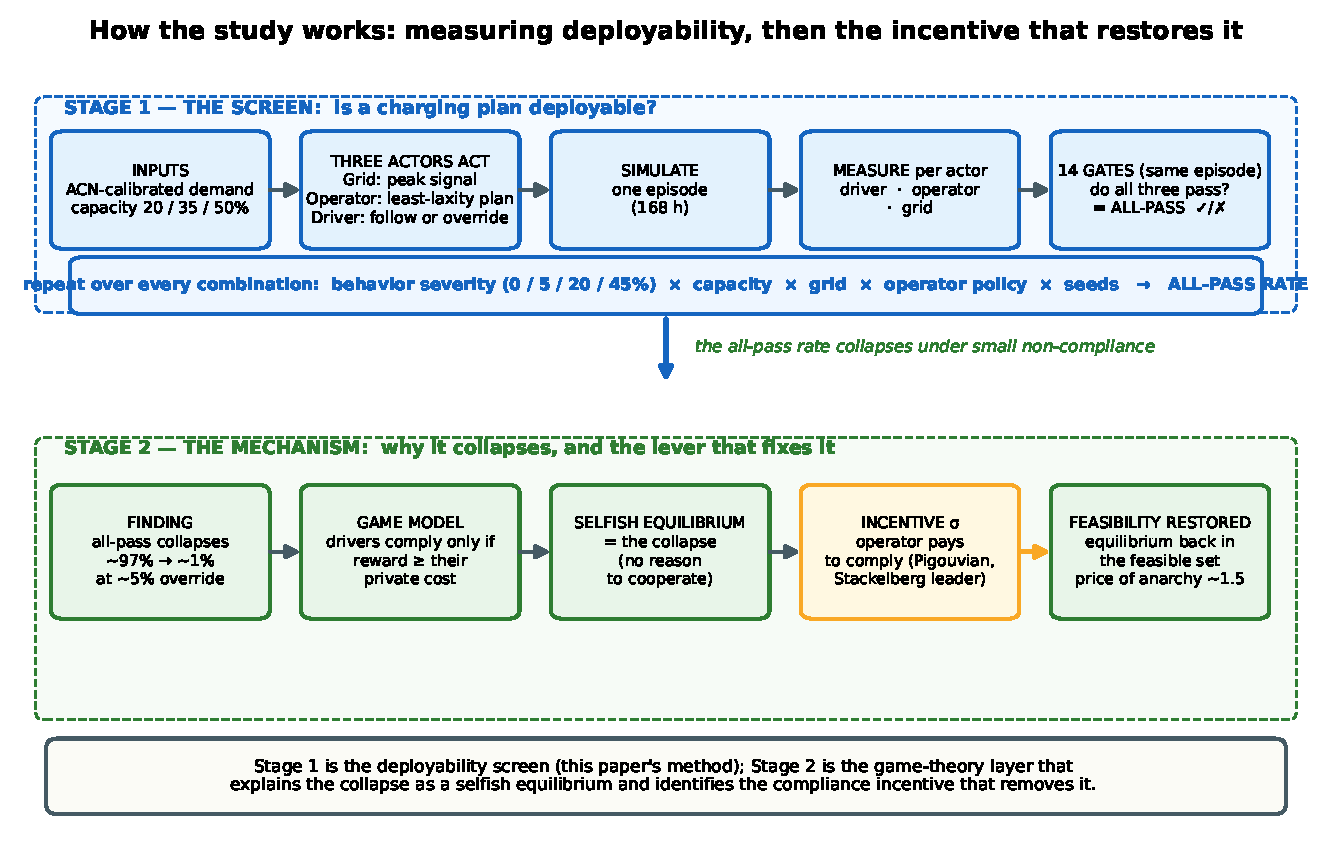
\includegraphics[width=0.68\textwidth]{figures/fig1_multi_actor_framework.pdf}
\caption{Multi-actor EV charging evaluation framework. The figure summarizes the screening logic: a policy is screened as acceptable under this study's gates only when the driver, charging operator, and grid gates pass simultaneously.}
\label{fig:framework}
\end{figure}

\section{Multi-actor acceptability formulation}\label{sec:formulation}

Let $i \in \mathcal{I}$ index EVs, $t \in \mathcal{T}$ index hourly simulation steps, $s \in \mathcal{S}$ index random seeds, $c \in \mathcal{C}$ index capacity levels, $b \in \mathcal{B}$ index behavior models, $f \in \mathcal{F}$ index operator policies, and $g \in \mathcal{G}$ index grid policies. A simulation episode is denoted $e=(s,c,b,f,g,H)$, where $H$ is the horizon.

The driver layer produces a request event set
\begin{equation}
\mathcal{R}_t = \{r: a_r=t, E_r^{req}>0, d_r \geq t\},
\label{eq:requestset}
\end{equation}
where $a_r$ is the event time, $E_r^{req}$ is the requested energy represented by the simulator event, and $d_r$ is a deadline or service-risk proxy when available. The request audit adds unique identifiers and retry links. A targeted demanded-kWh trace further records simulator demand sessions using the operational balance
\begin{equation}
E^{dem}_{i,t}=\max\left(E^{target}_{i,t},E^{deadline}_{i,t}\right),
\label{eq:demkwh}
\end{equation}
with explicit delivered, remaining, released, and unserved kWh terms. That trace supports event-level behavioral interpretation, but not field-observed energy-demand amplification.

The operator policy selects a recommended service action
\begin{equation}
x_{r,t}^F = \pi_f(r,t,\theta_f), \quad r \in \mathcal{R}_t,
\label{eq:fleetpolicy}
\end{equation}
subject to a capacity constraint
\begin{equation}
\sum_{r \in \mathcal{R}_t} p_r x_{r,t}^F \leq C_c,
\label{eq:capacity}
\end{equation}
where $p_r$ is the event charging power and $C_c$ is the capacity level. The grid policy modifies the operator recommendation:
\begin{equation}
x_{r,t}^G = \pi_g(x_{r,t}^F,L_t,P_t,\theta_g),
\label{eq:gridpolicy}
\end{equation}
where $L_t$ is site load and $P_t$ is a peak-pressure or price-related signal. The final served action is $x_{r,t}=x_{r,t}^G$. PeakPenalty is thus a grid-layer intervention, not evidence of a operator-layer idling mechanism.

Driver acceptability is represented as
\begin{equation}
A_D(e)=\mathbb{1}\left[ \rho_E(e)\geq \tau_E,\; \Delta_R(e)\geq \tau_R,\; \eta_D(e)\leq \tau_U \right],
\label{eq:drivergate}
\end{equation}
where $\rho_E$ is delivered-energy ratio, $\Delta_R$ is reliability delta relative to a reference, and $\eta_D$ is an unmet or requested-but-not-delivered event metric when available (distinct from the driver \emph{utility} $U_D$ of the game-theoretic analysis in Section~\ref{sec:game}, which is \emph{increasing} in service; the gate metric $\eta_D$ is a shortfall that is small when service is good). Operator acceptability is
\begin{equation}
A_O(e)=\mathbb{1}\left[ S_F(e)\geq \tau_S,\; Q_F(e)\leq \tau_Q,\; K_F(e)\leq \tau_K \right],
\label{eq:fleetgate}
\end{equation}
where $S_F$ is service completion, $Q_F$ is queue or request-volume pressure, and $K_F$ is a cost or operating penalty proxy. Grid acceptability is
\begin{equation}
A_G(e)=\mathbb{1}\left[ \rho_P(e)\leq \tau_P,\; \rho_{ramp}(e)\leq \tau_{ramp},\; \Delta LF(e)\geq \tau_{LF} \right],
\label{eq:gridgate}
\end{equation}
with peak ratio $\rho_P$, ramp ratio $\rho_{ramp}$, and load-factor change $\Delta LF$. The load-factor criterion $\Delta LF \geq -0.05$ should be read as ``load factor must not decline by more than $5$ percentage points relative to the anchor'': a negative $\Delta LF$ means a lower (worse) load factor than LeastLaxity, so the gate passes only when load factor is held within $5$ points of the anchor. In Eqs.~\eqref{eq:drivergate}--\eqref{eq:gridgate}, the indicator equals one only when all subcriteria for that actor pass in the same episode; for readability these equations show the representative subcriteria, while the full pre-specified set actually evaluated---three driver, six operator, and five grid criteria (14 in total)---is enumerated in Table~\ref{tab:gates}. Overall acceptability is
\begin{equation}
A_{all}(e)=A_D(e)A_O(e)A_G(e).
\label{eq:allgate}
\end{equation}
Thus, all-pass acceptability is a same-episode logical AND of driver, charging operator, and grid gates. Read game-theoretically, each actor gate is that actor's \emph{participation (individual-rationality) constraint}: the minimum standard at or above which the actor is willing to take part in the managed-charging program. An episode is then \emph{feasible} when all three participation constraints hold jointly, the all-pass indicator is the feasibility indicator, and the all-pass \emph{rate} over episodes is the empirical share of feasible episodes---a design-conditional, chance-constraint-style measure of deployability that, unlike a blended objective, does not let one actor's surplus offset another's shortfall. Equations~\eqref{eq:drivergate}--\eqref{eq:allgate} are normative gates rather than physical laws. To be precise about the distinction: all fourteen acceptability criteria are \emph{normative} operational thresholds chosen by us (service ratios, waiting limits, load-shape ratios), not hard physical limits. The one genuinely \emph{physical} constraint we consider---distribution-feeder voltage feasibility---is deliberately \emph{not} one of the fourteen gates; it enters only through the separate IEEE-33 screen (Section~\ref{sec:results}), where it is base-load-determined and non-binding. The exportable part of the framework is therefore the normative-gate structure, and which specific thresholds a deployer adopts is a stakeholder choice. Their value is transparency: when a conclusion changes under a threshold sweep, the manuscript reports the conclusion as threshold-conditioned rather than robust in a threshold-independent sense.

This makes explicit how the screen relates to optimization rather than replacing it. A conventional design minimises a blended objective $\min_x J(x)=\alpha J_D(x)+\beta J_O(x)+\gamma J_G(x)$, which is \emph{compensatory}: a large gain in one actor's term can offset another's shortfall in the aggregate score. The feasibility screen instead asks whether a candidate policy lies in the jointly-feasible set $\mathcal{F}=\{x: A_D(x)=A_O(x)=A_G(x)=1\}$. The two combine naturally---the deployable design problem is
\begin{equation}
\min_x\; J(x)\quad\text{subject to}\quad A_D(x)=A_O(x)=A_G(x)=1,
\label{eq:optwithin}
\end{equation}
i.e.\ optimisation \emph{within} the feasible set: optimisation chooses an efficient point, and the gates decide whether that point is jointly deployable. Formally the gates are nothing more than the constraint set of this optimisation, so we do not claim deployment lies \emph{outside} optimisation; the claim is narrower and structural---that the \emph{constraint set}, not the objective, is the primary object for deployment, with the objective secondary and evaluated only within it. The screen is thus a complement to, not a substitute for, optimisation, and its distinctive role is to expose policies that are objective-optimal yet infeasible (Section~\ref{sec:results}).

We make no claim these fourteen criteria are \emph{complete}; they are a representative selection of each actor's principal operational concern (driver service/reliability; operator queueing/waiting/cost; grid load-shape), with the count set by sub-concerns (three driver, six operator, five grid), not a target number. Excluded candidates (reactive power, harmonics, a separate driver charging-cost gate) need a power-electronics or tariff model beyond scope, and some are partly captured already (price sensitivity via the cheap-window behavior, operator cost via the cost gates). Adding further conjunctive gates cannot raise the all-pass rate: because the feasible set is a \emph{conjunction}, the all-pass rate is monotonically non-increasing in the number of gates, so a more complete set would make feasibility \emph{lower} and the collapse sharper, never higher. The numerical result is thus conservative to added constraints, although the substantive validity of the screen still depends on choosing representative actor criteria and defensible thresholds. As for redundancy, although some criteria are correlated by construction, the four \emph{binding} criteria are not mutually collinear---critical-requested-not-delivered (driver), 95th-percentile wait (operator), and the squared-load and ramp ratios (grid), measuring service, waiting, and load shape respectively---so dropping any one would not collapse the result (Section~\ref{sec:robust}).

\begin{table}[t]
\centering
\caption{Pre-specified actor-gate thresholds used in this study.}
\label{tab:gates}
\scriptsize
\begin{tabularx}{\textwidth}{p{0.12\textwidth}Yp{0.13\textwidth}p{0.14\textwidth}Y}
\hline
Actor & Metric & Pass & Threshold & Unit or interpretation \\
\hline
Driver & Delivered ratio vs LeastLaxity anchor & $\geq$ & 0.95 & ratio \\
Driver & Reliability delta vs anchor & $\geq$ & -0.5 & percentage points \\
Driver & Critical requested-not-delivered delta vs anchor & $\leq$ & 24 & events \\
Operator & Requested-not-delivered delta vs anchor & $\leq$ & 117 & events \\
Operator & Mean queue delta vs anchor & $\leq$ & 1.0 & vehicles or queue units \\
Operator & Max queue delta vs anchor & $\leq$ & 2.0 & vehicles or queue units \\
Operator & 95th percentile wait delta vs anchor & $\leq$ & 30 & minutes \\
Operator & Energy-cost ratio vs anchor & $\leq$ & 1.10 & ratio \\
Operator & Demand-charge exposure ratio vs anchor & $\leq$ & 1.10 & ratio \\
Grid & Peak ratio vs anchor & $\leq$ & 1.05 & ratio \\
Grid & Ramp p95 ratio vs anchor & $\leq$ & 1.10 & ratio \\
Grid & Peak-to-average ratio vs anchor & $\leq$ & 1.10 & ratio \\
Grid & Squared-load proxy ratio vs anchor & $\leq$ & 1.10 & ratio \\
Grid & Load-factor delta vs anchor & $\geq$ & -0.05 & signed delta \\
\hline
\end{tabularx}
\end{table}

The driver gates represent service adequacy, reliability, and critical unmet service. Delivered-energy ratio captures whether the controller provides enough energy relative to the LeastLaxity anchor, while reliability and critical requested-not-delivered events represent the service-quality risks that are central to EV charging facility operation \cite{woo2021,danner2021} and managed-charging acceptance \cite{will2016,bailey2015,schmalfuss2015,delmonte2020,tarroja2021}. The cited literature motivates service and acceptance as gate families; it does not establish the exact numeric thresholds as universal constants. The reliability-delta gate is intentionally tight relative to the delivered-energy gate, so driver failures can be triggered by small reliability losses even when aggregate delivered energy remains high.

The operator gates represent operational burden. Queue and waiting metrics measure whether charging decisions increase operational congestion, requested-not-delivered events measure service-completion risk, and cost and demand-charge exposure represent the operator's economic acceptability. These gates follow the cost-service trade-off perspective used in EV charging facility evaluation \cite{woo2021}, but the thresholds are pre-specified normative criteria for this simulation campaign.

The grid gates represent load-shape discipline. Peak ratio, ramp ratio, peak-to-average ratio, squared-load proxy, and load-factor change capture whether a policy shifts stress toward the distribution system or worsens the aggregate site profile. Distribution-impact studies motivate the use of voltage, loading, losses, and load-shape metrics \cite{clement2010,elnozahy2014,green2011,muratori2018,dubey2015,pieltain2011,powell2022}. The grid gate itself is evaluated at the site level from these load-shape metrics. Separately, an IEEE-33 feeder screen (Section~\ref{sec:results}) is used as an external grid-stress lens: it is not used to define the actor gates but to translate each charging policy's load profile into representative distribution-feeder deltas relative to an EV-off baseline \cite{baran1989,thurner2018,pandapowerdoc}.

When a submetric is unavailable in a specific run, it is not silently counted as a pass; the reported gate is computed from the recorded simulation outputs. The threshold families themselves are grounded in established constructs: delivered-energy ratio and critical requested-not-delivered events are standard charging service-quality and reliability measures \cite{woo2021,danner2021,tan2023fair}, queue and 95th-percentile wait deltas are standard waiting-time service metrics \cite{tan2023fair,theodoropoulos2022proportional}, and peak, ramp, and load-factor ratios are standard distribution load-shape stress measures \cite{clement2010,muratori2018,powell2022}. The exact numeric cut-points, however, are fixed normative scenario criteria rather than literature-derived constants; the threshold sensitivity analysis is included because these values are normative and could be disputed, and the decomposition in Section~\ref{sec:robust} reports which of them actually bind. The thresholds are pre-specified normative criteria, not universal constants. Threshold sensitivity is therefore used to expose dependence on those normative choices rather than to claim threshold-independent robustness. In the weekly 168 h sensitivity file, tightening the delivered-ratio threshold from 0.95 to 0.99 reduces all-pass count by 18 rows, and requiring 1.00 reduces it by 60 rows.

\subsection{Policy families}

The diagnostic baselines are LeastLaxity, CostOnly, and QueueAware. LeastLaxity (least-laxity-first scheduling, which serves the cars with least deadline slack first) is the anchor because it is near-optimal for deadline-driven service: under full compliance it achieves $93.6\%$ trip reliability with essentially zero 95th-percentile queue wait, so passing a relative driver gate (delivered-energy ratio $\geq0.95$ of LeastLaxity) means genuinely high absolute service, not a low bar; relative gates isolate \emph{degradation under behavior} from absolute level, and a weaker anchor would only make the gates easier. LeastLaxity plays two roles that are not circular: the fixed \emph{reference} for the relative gates (computed once under full compliance and held fixed, so the gates measure degradation against a fixed target) and one deployable \emph{scheduler} among those evaluated---and re-running the entire screen with an Earliest-Deadline-First anchor reproduces the same threshold (Section~\ref{sec:robust}, ``Sixth''), so the result is not an artifact of that choice. Our behavioral model applies non-compliance at \emph{action selection} (drivers override the recommended action) while the deadline and energy-need inputs to the laxity computation stay truthful; we do not model \emph{information-level} misreporting, which would degrade LeastLaxity further, so our results are a conservative reading. CostOnly and QueueAware are diagnostic single-objective heuristics, not state-of-the-art algorithms.

FleetServiceFirst uses the simulator's LeastLaxity action rule and prioritizes service completion and reliability. FleetServiceGridWeighted starts from the LeastLaxity action vector and defers at most $20\%$ of the already-recommended \emph{flexible, low-risk} requests when a queue, peak, or price trigger is active, adding no new requests. It is a transparent robustness comparator---not a proposed controller---included only to test whether the behavioral result depends on the ServiceFirst baseline or on a particular weighting; its scoring weights and term definitions are given in Supplementary Material~\ref{sec:supp} (Eqs.~\eqref{eq:sgwservice}--\eqref{eq:sgwpriority}, Table~\ref{tab:sgwterms}).

The defense of this comparator does not rest on the weight values. Critical, low-SoC, and deadline-risk requests are excluded from the deferral-eligible set by construction, so no grid-pressure weight, however large, can defer them; the coefficients only order the already-flexible, low-risk candidates among themselves. The screening result is therefore insensitive to the weights: a six-variant coefficient ablation---including a variant with all weights set equal, which removes the ordering entirely---leaves the conclusion unchanged (Supplementary Material~\ref{sec:supp}). ServiceGridWeighted is thus a fixed-scalarization robustness check, not a tunable acceptability model or a superior controller.

\subsection{Algorithm}

Algorithm~1 summarizes the multi-actor gate-evaluation workflow: for each episode it generates driver request events, applies the operator and grid policies, simulates final service, and scores the driver, charging operator, grid, and all-pass gates.

\begin{figure}[t]
\centering
\fbox{\begin{minipage}{0.92\textwidth}
\textbf{Algorithm 1. Multi-actor gate evaluation}\par\smallskip
\textbf{Input:} seeds $\mathcal{S}$, capacities $\mathcal{C}$, behaviors $\mathcal{B}$, operator policies $\mathcal{F}$, grid policies $\mathcal{G}$, horizon $H$.\par
\begin{enumerate}
    \item For each episode $e=(s,c,b,f,g,H)$, generate driver request events with unique request identifiers.
    \item Apply the operator policy to obtain recommended charging actions.
    \item Apply the grid policy to obtain adjusted charging actions.
    \item Simulate final service, deferral, and unserved outcomes.
    \item Record driver, charging operator, and grid metrics.
    \item Compute $A_D(e)$, $A_O(e)$, $A_G(e)$, and $A_{all}(e)$.
    \item Assign a failure pattern from the three actor gates.
    \item Aggregate pass rates, request-event ratios, feeder deltas, and threshold sensitivity.
\end{enumerate}
\textbf{Output:} actor-gate matrix, failure taxonomy, audit tables, and reproducible figures.
\end{minipage}}
\end{figure}

\section{Experimental design}\label{sec:design}

The experimental workflow combines simulation runs with targeted trace checks. The request-ID trace verifies that each request event has a unique identifier, counts reconcile through the driver, charging operator, grid, and final-service pipeline, and retries are represented explicitly. A subsequent demanded-kWh trace runs the targeted 28-day severity design, persists demand sessions, and reconciles the identity
\begin{equation}
E^{rem}_{pre}+E^{new}=E^{delivered}+E^{rem}_{post}+E^{release}
\label{eq:ledger}
\end{equation}
within $10^{-4}$ kWh. Here $E^{rem}_{pre}$ and $E^{rem}_{post}$ are outstanding simulator demanded kWh before and after a vehicle step, $E^{new}$ is newly created demanded kWh, $E^{delivered}$ is charging credited to outstanding demand, and $E^{release}$ is a demand reduction not explained by delivered charging. The actual/operator request-event ratio is $\chi=N^{actual}/N^F$, where $N^F$ counts operator-recommended request events before grid-layer adjustment and $N^{actual}$ counts final driver-layer request events. Under full compliance, drivers follow grid-adjusted recommendations; therefore $\chi$ can be below one when the grid layer defers a subset of operator recommendations. This explains why the weekly severity-0 mean is 0.984 rather than exactly 1.000.

The weekly severity sweep uses four parameterized behavior levels. At each vehicle-timestep, the driver keeps the grid-adjusted operator recommendation with probability $p_{keep}$. If the recommendation is not kept, the vehicle follows a reserve/price-window recommendation-override preference created from simulator state: SoC, anxiety threshold $\theta$, target deficit, deadline deficit, action availability mask, deadline laxity, and a time-of-use cheap-window indicator. The reserve threshold is $\theta$ plus the severity-specific reserve margin, with the cheap-window extra margin added during low-price windows. The noncompliant preference uses the score
\begin{equation}
260C_i + 130N_i + 95T_i + 55D_i + 35(1-SoC_i)-10\ell_i,
\label{eq:severitypref}
\end{equation}
where $C_i$ is the cheap-window indicator, $N_i$ the reserve need, $T_i$ the target-SoC deficit, $D_i$ the deadline deficit, $SoC_i$ the state of charge, and $\ell_i$ the normalized laxity, and then applies the existing capacity-limited selector. Every term is normalized to $[0,1]$, so the six coefficients are \emph{dimensionless utility weights} and the score is an ordinal utility index, not a physical quantity; only their relative ordering and ratios matter, and the result's robustness to them (all-weights-equal, $\pm50\%$) is shown in Section~\ref{sec:robust}. The preference's \emph{term structure} is grounded in behavioral evidence: the reserve-seeking term reflects charge/range anxiety \cite{schmalfuss2015,hardman2018,will2016}, the cheap-window term time-of-use price sensitivity \cite{bailey2025fieldexp,delmonte2020,marxen2023flexibility}, and the deadline/laxity terms the finding that drivers prioritize charging and opt out when they need their vehicle soon \cite{alexeenko2023pilot,dudek2021electricnation}; the additive-linear form is the deterministic-utility component of a multinomial-logit choice, the standard travel/charging-behavior model \cite{mcfadden1974,daina2017}. The five behavior types in the full matrix (recommendation-override, limited-attention, price-sensitive, SoC-compliance, SoC-queue-compliance) are operationalizations of this one preference under different keep-probability $p_{keep}$ and margin settings (Table~\ref{tab:severityparams}).

These severity levels are stress-test brackets, not calibrated forecasts. Field studies report per-event opt-out in the tens of percent---OptimizEV session-level opt-in near $60\%$ (toward $90\%$ opt-out at low slack) \cite{alexeenko2023pilot}, active override in Electric Nation \cite{dudek2021electricnation}, and near-full reversion once incentives are withdrawn \cite{bailey2025fieldexp,wong2023incentives,marxen2023flexibility}---against which severity~1 ($5\%$) is intentionally low, severity~2 ($20\%$) sits within reported ranges, and severity~3 ($45\%$) is an upper boundary; the validation ACN-Data itself shows $\sim$33\% early disconnection and 72\% departure mismatch across 29{,}116 sessions, so $5\%$ is low relative to observed deviation. This is a plausibility bracket, not a calibration---the severity parameter acts at the vehicle-timestep level whereas field evidence reports per-session opt-out---and the headline triggers already at severity~1, independent of the higher settings.

\begin{table}[p]
\centering
\caption{Behavioral severity parameters implemented in the direct multi-actor severity sweep.}
\label{tab:severityparams}
\tiny
\begin{tabularx}{\textwidth}{p{0.06\textwidth}p{0.13\textwidth}p{0.19\textwidth}Yp{0.16\textwidth}p{0.16\textwidth}}
\hline
Severity & Label & Parameter values & Mechanism changed & Intended interpretation & Evidence boundary \\
\hline
0 & full\_compliance & $p_{keep}=1.00$; reserve margin 0.00; cheap-window extra 0.00 & Actual action equals grid-adjusted recommendation & Upper-bound benchmark & Not a field forecast \\
1 & low\_deviation & $p_{keep}=0.95$; reserve margin 0.05; cheap-window extra 0.10 & 5\% of vehicle-timesteps use reserve-seeking recommendation-override; cheap windows raise reserve threshold by 0.10 & Small noncompliance stress test & Not calibrated to observed opt-out rates \\
2 & moderate\_deviation & $p_{keep}=0.80$; reserve margin 0.15; cheap-window extra 0.30 & 20\% recommendation deviation with stronger reserve and cheap-window recommendation-override & Intermediate stress test & Not calibrated to field behavior \\
3 & severe\_deviation & $p_{keep}=0.55$; reserve margin 0.25; cheap-window extra 0.60 & 45\% recommendation deviation with cheap-window request herding & Boundary stress case & Not realistic without calibration \\
\hline
\end{tabularx}
\end{table}

Table~\ref{tab:sevanchor} maps the three deviation levels to the per-event opt-out and override magnitudes reported in published managed-charging field studies, positioning them as literature-anchored scenario severities rather than calibrated behavioral estimates.

\begin{table}[t]
\centering
\caption{Literature anchoring of the behavioral severity levels. Deviation magnitudes are positioned against per-event opt-out, override, and reversion evidence from managed-charging field studies; this anchors the scenarios but is not a population-specific calibration. The comparison is a plausibility bracket, not a conversion between directly comparable quantities: the field evidence reports per-session opt-out (a binary per-visit event) whereas the severity parameter $p_{keep}$ operates at the vehicle-timestep level, so the columns are not numerically interchangeable.}
\label{tab:sevanchor}
\begin{tabularx}{\textwidth}{p{0.10\textwidth}p{0.12\textwidth}X}
\hline
Severity & Deviation & Field-evidence anchor and role \\
\hline
1 (low-deviation) & $\sim$5\% & Below typical observed per-event opt-out ($\sim$16--40\% in residential managed-charging pilots \cite{alexeenko2023pilot,dudek2021electricnation}); an optimistic, low-friction case. \\
2 (moderate) & $\sim$20\% & Within the observed per-event opt-out range; a central case consistent with pilot evidence \cite{alexeenko2023pilot}. \\
3 (severe) & $\sim$45\% & Above routine observation; representative of low-flexibility sessions (opt-out toward $\sim$90\% \cite{alexeenko2023pilot}) or of near-full reversion once incentives are withdrawn \cite{bailey2025fieldexp}; an adverse boundary case. \\
\hline
\end{tabularx}
\end{table}

The weekly sweep uses capacities of 20\%, 35\%, and 50\%, ServiceFirst and ServiceGridWeighted policies, and NoGridAdjustment and GridPeakPenalty variants. Capacity here is a fraction of the site's base charger provision: $35\%$ and $20\%$ correspond to roughly one served charger per three and per five concurrently demanding vehicles, which sit within the realistically constrained range for shared workplace and depot charging (installed port-to-vehicle ratios of about $1{:}5$ to $1{:}20$ \cite{muratori2018,powell2022}), while $50\%$ is comparatively well provisioned; these are constrained but not pathological regimes, quantified in Section~\ref{sec:data}. The design is deliberately a \emph{full factorial} over (behavior severity $\times$ charger capacity $\times$ grid policy $\times$ operator policy) rather than a one-factor-at-a-time sweep, because the central claim is about a same-episode \emph{interaction}---whether behavioral deviation breaks feasibility \emph{regardless of} the infrastructure and policy context---which can only be established by crossing the behavioral factor with the deployment factors and confirming the collapse in every cell. The factorial also lets the diagnostic disaggregation (Section~\ref{sec:diagnostic}) attribute residual feasibility to specific capacity and gate combinations, which a marginal sweep would confound. The full actor-gate matrix, including the diagnostic CostOnly and QueueAware baselines, uses five seeds; the reported severity and robustness results use a 20-seed expansion (seeds 4541--4560) of the service-oriented family, giving 240 episodes per severity level. The targeted 28-day confirmation uses a 672 h horizon, seeds 4541--4545, 35\% capacity, LeastLaxity, ServiceFirst, ServiceGridWeighted, and both grid policies.

The IEEE-33 screen uses 900 weekly cases and 151,200 hourly power-flow solves. It includes 15 policies, three capacities, 10 seeds, two placements, and a 168 h horizon. The placement cases are concentrated bus 18 and distributed buses 18/22/25/30/33. Voltage results are treated as a boundary condition because EV-off baseline conditions dominate absolute voltage violation counts. The useful feeder evidence is the relative change in substation peak, line loading, and losses versus EV-off and LeastLaxity anchors.

\section{Data and simulation setup}\label{sec:data}

The simulator uses hourly resolution; weekly experiments use 168 h and the targeted confirmation 672 h. The primary weekly evidence contains 300 explicit actor-gate rows; the targeted 28-day evidence contains 85 rows (80 severity-policy-grid combinations plus five LeastLaxity anchor rows). Random seeds are fixed and reported in the reproducibility appendix. Here $100\%$ capacity denotes the site's base charger provision (40 home, 5 work, 5 public slots per location group); the weekly levels of 20/35/50\% are fractions of that base, sitting within the realistically constrained range for shared workplace/depot charging justified in Section~\ref{sec:design}, with the most dramatic results in the more constrained settings.

The grid layer compares two settings, \emph{NoGridAdjustment} and \emph{GridPeakPenalty} (shown as \textsf{NoGrid} and \textsf{PeakPenalty} in the figures). Under NoGridAdjustment the grid sends no signal and the charging operator's recommendations pass through unchanged. Under GridPeakPenalty the grid discourages a high coincident charging peak---concretely it adds a peak term $J_G=\lambda_P\max_t P_t$ to the schedule objective, so flexible load is pushed off the busiest hour; the deferrals this produces are attributed to the grid layer, not to the charging-operator heuristic. Both settings describe only whether the grid \emph{adjusts the recommended schedule}; neither pays drivers, so grid adjustment and driver incentives stay separate. (We rename the earlier `NoGridIncentive' label to NoGridAdjustment for exactly this reason: it never involved a payment.)

\subsection{External validation of the charging-demand model}\label{sec:extval}

While the behavioral severity layer is a stress-test construct, the underlying charging-demand model is not synthetic: it is calibrated to real charging data. The workplace scenario draws each session's delivered energy, dwell duration, and arrival hour from distributions fitted to the public Adaptive Charging Network (ACN) dataset \cite{acndata2019}, combining the Caltech, JPL, and Office001 sites over twelve months ($n=29{,}149$ cleaned sessions; the $29{,}116$ sessions with complete energy, dwell, and arrival features are used for the distributional comparison in Table~\ref{tab:extval}). The delivered-energy and dwell distributions are lognormal fits whose parameters are used directly by the simulator; the arrival-hour distribution is the empirical ACN connection-hour histogram.

We validate the simulator at the output level by comparing 3{,}435 generated sessions (eight seeds) to the real ACN sessions via Kolmogorov--Smirnov (KS) and 1-Wasserstein distances (Table~\ref{tab:extval}, \figref{fig:extval}). Delivered energy agrees closely (KS $=0.087$; means 11.65 vs 12.17 kWh), arrival hour after aligning the dataset's UTC timestamps to local time (KS $=0.068$), and dwell reasonably (KS $=0.176$). The simulator's 40 kWh energy clip and 14 h dwell cap truncate the heaviest real sessions, slightly under-representing extreme-demand tails---yet severity-dependent failures appear even under this capped demand, so the mechanism is not driven by extreme sessions. An independent ACN-Sim \cite{lee2019acnsim} cross-check on the real Caltech network gives mean energy 12.19 kWh versus our 11.65 and the data's 12.17 (within $\sim$4\%); the gap is the expected consequence of our deliberate tail cap (ACN-Sim applies none) and clears our pre-stated $\pm10\%$ validation criterion---conventional for demand models and consistent with ACN-Sim's own run-to-run sensitivity---which suffices because the framework studies \emph{relative} degradation under behavior. The grid layer is likewise grounded: power flow is solved with the validated pandapower package \cite{thurner2018,pandapowerdoc} on the Baran--Wu IEEE-33 feeder \cite{baran1989}. The remaining external-validity gap is therefore not the demand or grid-physics model but the behavioral-response layer, bracketed against field evidence (Section~\ref{sec:design}) rather than fitted.

\begin{table}[t]
\centering
\caption{External validation of the simulator's generated charging sessions against real ACN-Data (Caltech/JPL/Office, $n_{\mathrm{real}}=29{,}116$; $n_{\mathrm{sim}}=3{,}435$). KS is the two-sample Kolmogorov--Smirnov distance (smaller is closer).}
\label{tab:extval}
\begin{tabular}{lccccc}
\hline
Session variable & Sim mean & Real mean & KS & Wasserstein \\
\hline
Delivered energy (kWh) & 11.65 & 12.17 & 0.087 & 0.98 \\
Dwell duration (h) & 6.60 & 6.68 & 0.176 & 1.20 \\
Arrival hour (local-time aligned) & 9.76 & 10.02 & 0.068 & 0.26 \\
\hline
\end{tabular}
\end{table}

\begin{figure}[t]
\centering
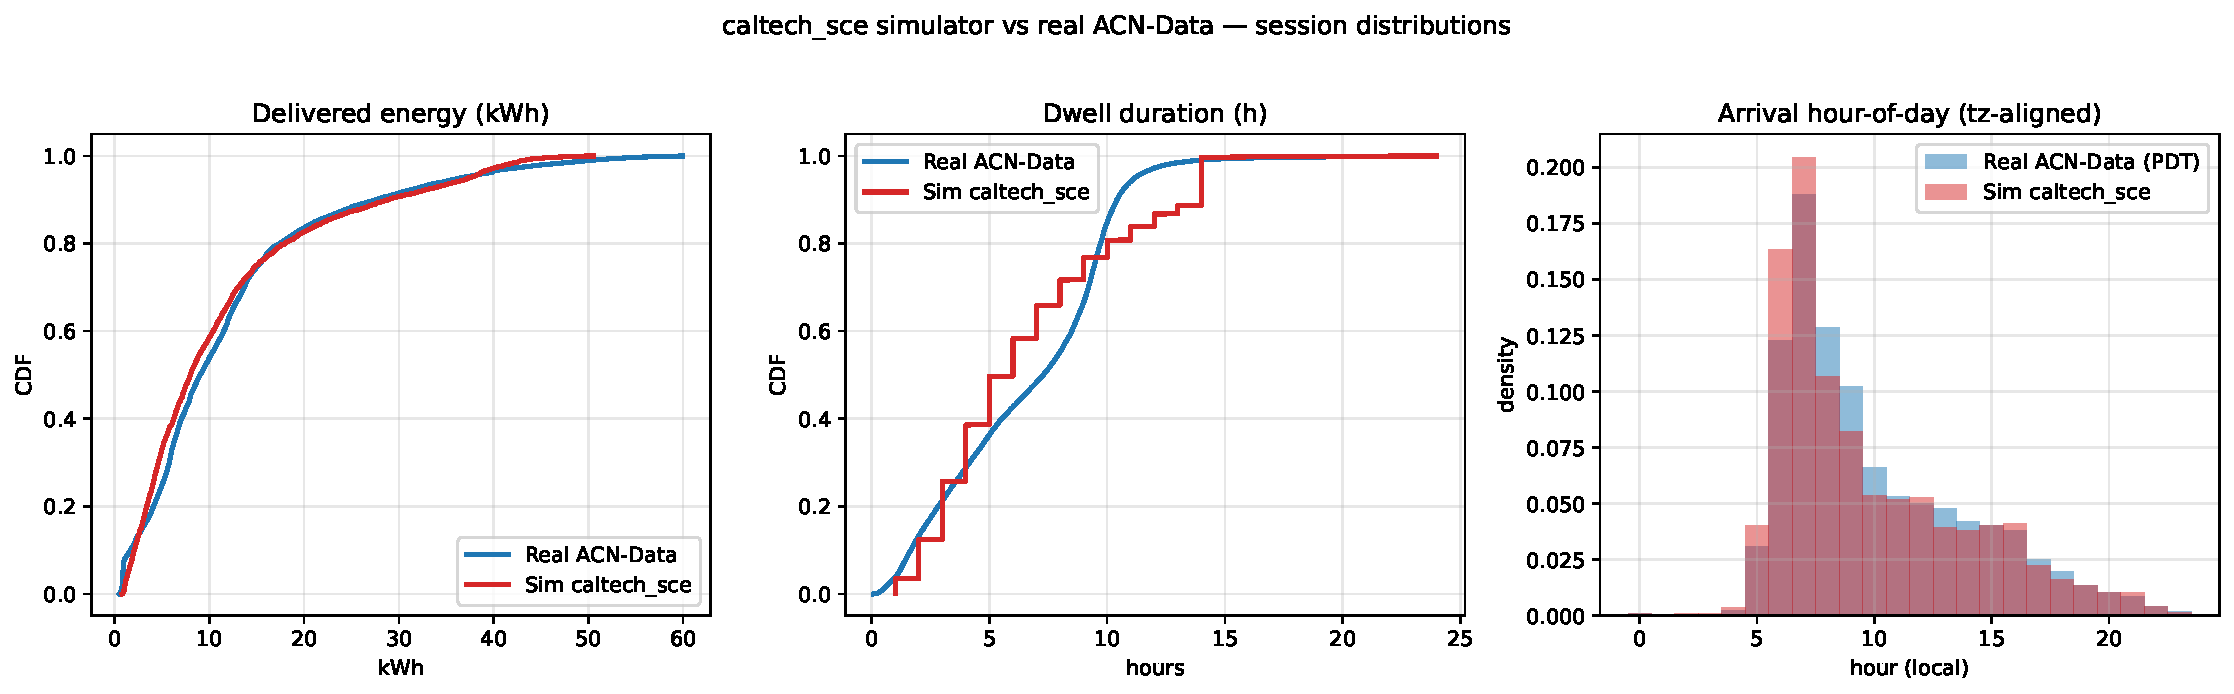
\includegraphics[width=0.74\textwidth]{figures/acn_validation_overlay_20260615.pdf}
\caption{Generated simulator sessions (red) versus real ACN-Data (blue). Cumulative distributions of delivered energy and dwell duration and the arrival-hour histogram (local-time aligned) reproduce the central mass of the real distributions, while under-representing some extreme tails (Section~\ref{sec:extval}).}
\label{fig:extval}
\end{figure}

Finally, we test whether the headline result depends on the specific demand distribution by redrawing the per-session energy and dwell from each \emph{independent} real ACN site---Caltech, JPL, and Office001---using that site's own fitted parameters in place of the combined fit, and re-running the severity-0 and severity-1 service-oriented check (35\% capacity, both grid policies, five seeds). The severity-1 collapse reproduces under every demand distribution: same-episode all-pass is 0.000 at severity~1 for the combined fit and for all three individual sites. Under full compliance, all-pass is 1.000 for the combined, Caltech, and JPL demand and 0.900 for the highest-energy Office001 demand, where the two residual misses are grid load-shape trips rather than service failures, consistent with the capacity-dependent grid-gate behavior reported in Section~\ref{sec:robust}. The behavioral collapse is therefore not an artifact of one demand model; it holds across three independent real charging populations. These three sites are all US workplace/campus charging contexts with similar morning-peaked arrival profiles, so this test establishes robustness to the demand \emph{magnitude} across real populations but not to qualitatively different arrival distributions; generalization to residential overnight, public fast-charge, or non-US arrival patterns is left to future work.

\section{Results}\label{sec:results}

\subsection{Actor gates change which policies look successful}

\figref{fig:matrix} states the main result directly. Panel (A) condenses the service-oriented family (both ServiceFirst and ServiceGridWeighted, all capacities and grid policies) to a behavior-severity by actor-gate heatmap; the highlighted right-hand column is the all-pass conjunction. Panel (B) shows that the all-pass collapse is identical for both service-oriented operator policies. The single most important feature is that the all-pass (conjunction) gate falls to near zero at severity~1, one severity step before the individual driver, charging operator, and grid gates all reach zero: at severity~1 the individual gates still pass at 0.050, 0.188, and 0.321, yet almost no episode satisfies all three at once (all-pass 0.012). The full policy-by-behavior-by-grid actor-gate matrix, including the diagnostic CostOnly and QueueAware comparators, is provided as Supplementary \figref{fig:suppmatrix}; \tabref{tab:weeklymatrix} reports the aggregate per-policy pass rates. The service-oriented family passes the all-pass gate in 96.7\% of full-compliance episodes (20 seeds; 95\% bootstrap interval $[94.2\%, 98.8\%]$), collapsing to 1.2\% at severity~1 ($[0.0\%, 2.9\%]$; the two intervals do not overlap; see Section~\ref{sec:robust}), whereas CostOnly and QueueAware fail all three actor gates, and hence all-pass, in the weekly evidence. ServiceGridWeighted is included as a comparator robustness check, but it does not overturn the main result: the paper makes no controller-superiority claim.

\begin{figure}[t]
\centering
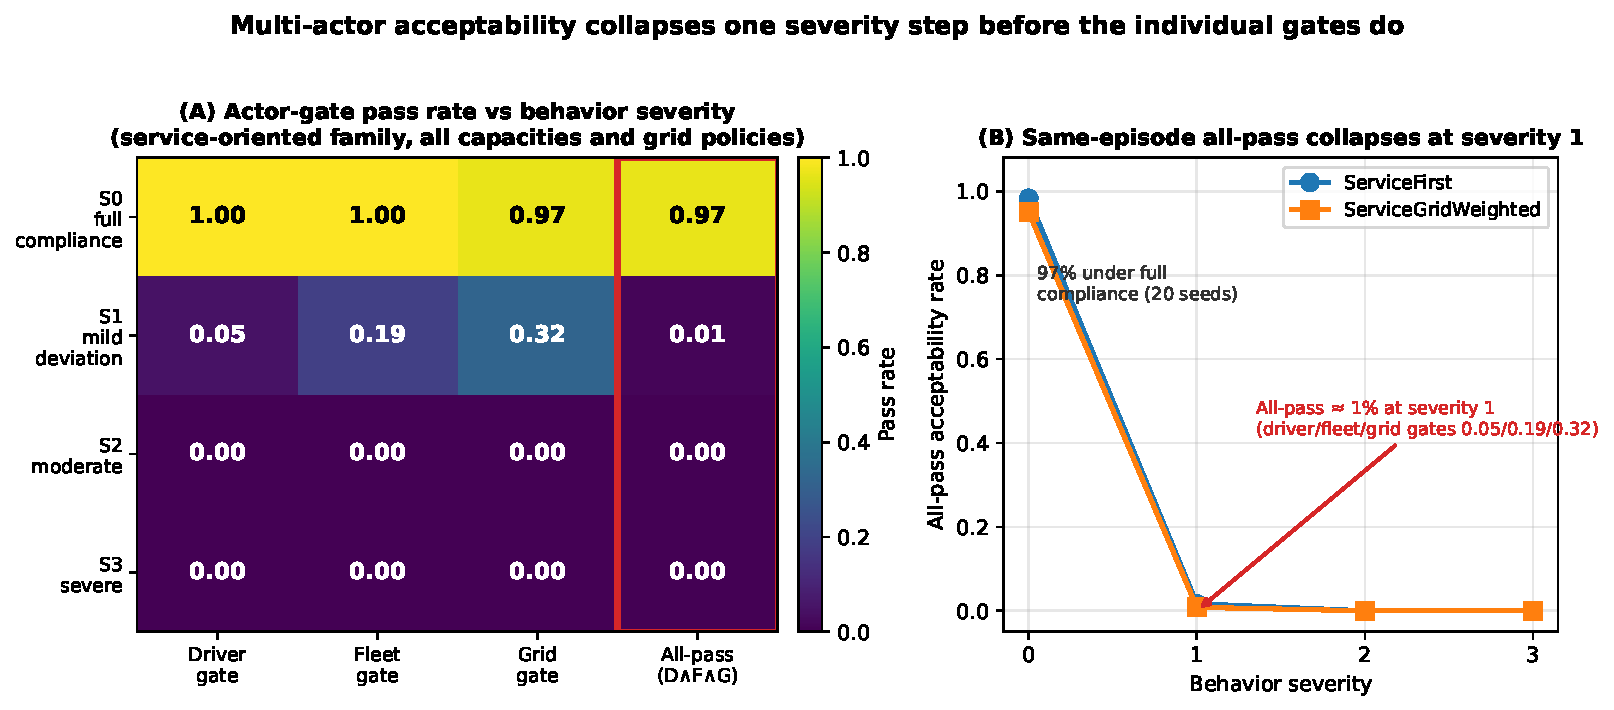
\includegraphics[width=0.82\textwidth]{figures/fig2_actor_gate_acceptability_matrix.pdf}
\caption{Multi-actor acceptability collapses one severity step before the individual gates do. (A)~Pass rate for the driver, charging operator, and grid gates and their all-pass conjunction (highlighted) as a function of behavior severity, averaged over the service-oriented operator policies, both grid policies, and all capacities. (B)~All-pass acceptability rate versus severity for ServiceFirst and ServiceGridWeighted; the two service-oriented policies are indistinguishable, and same-episode all-pass falls from 96.7\% under full compliance to 1.2\% at severity~1 even though the individual gates still pass at 0.050/0.188/0.321. Pass rates are 20-seed means across three capacities. Reading guide: read \emph{across severity} (left to right) for behavioral sensitivity, \emph{down the actor gates} (driver/operator/grid) for which actor constraint binds, and compare the highlighted all-pass row against the individual gate rows to see the conjunction fail before any single gate does. This is a joint-threshold result under the stated normative gates, not a physical discontinuity in charging service.}
\label{fig:matrix}
\end{figure}

\begin{table}[t]
\centering
\caption{Weekly actor-gate pass rates by operator policy (five-seed full matrix, including the diagnostic CostOnly and QueueAware baselines). The service-oriented rows are refined by the 20-seed expansion in Section~\ref{sec:robust}.}
\label{tab:weeklymatrix}
\begin{tabular}{lcccc}
\hline
Operator policy & Driver pass & Operator pass & Grid pass & All-pass \\
\hline
FleetCostOnly & 0.000 & 0.000 & 0.000 & 0.000 \\
FleetQueueAware & 0.000 & 0.000 & 0.000 & 0.000 \\
FleetServiceFirst & 0.250 & 0.300 & 0.342 & 0.250 \\
FleetServiceGridWeighted & 0.267 & 0.292 & 0.350 & 0.250 \\
\hline
\end{tabular}
\end{table}

CostOnly and QueueAware have all-pass rates of 0.0\% and 0.0\%. ServiceFirst and ServiceGridWeighted both have all-pass rates of 25.0\% and 25.0\%, respectively, because their all-pass outcomes occur under full compliance and disappear under behavioral deviation. The equal aggregate all-pass rate means ServiceGridWeighted should be read as a comparator check, not a superior controller. The main result is that service-oriented dispatch can be acceptable in favorable behavior conditions, but the actor gates expose failure when behavioral pressure increases.

\paragraph{Pareto efficiency does not imply same-episode acceptability.} This distinction from marginal- or scenario-averaged objective comparison is concrete, not only conceptual, and it appears already under full compliance. \figref{fig:pareto} plots each scheduling policy in the headline objective space of energy cost and trip reliability. CostOnly is \emph{Pareto-efficient}: it has the lowest energy-cost ratio ($0.955$) and the highest trip reliability ($94.5\%$) of any policy, and it \emph{dominates} the only acceptable policy, ServiceFirst, on both of these objectives (ServiceFirst: cost $1.004$, reliability $93.3\%$). A multi-objective optimizer or a Pareto-front analysis minimizing cost and maximizing reliability would therefore prefer CostOnly to ServiceFirst. Yet CostOnly's same-episode all-pass is $0.000$ versus ServiceFirst's $0.967$: in pursuing low cost it incurs a $30.9$-minute 95th-percentile wait and degrades critical-service delivery and load shape relative to the anchor, failing the driver, charging operator, and grid gates that an aggregate-objective view never imposes jointly per episode. The two objective-optimal policies (CostOnly, QueueAware) both score $0\%$, while the only acceptable policy is objective-dominated---a direct demonstration that per-episode multi-actor feasibility is not recoverable from a Pareto front over averaged objectives.

\begin{figure}[t]
\centering
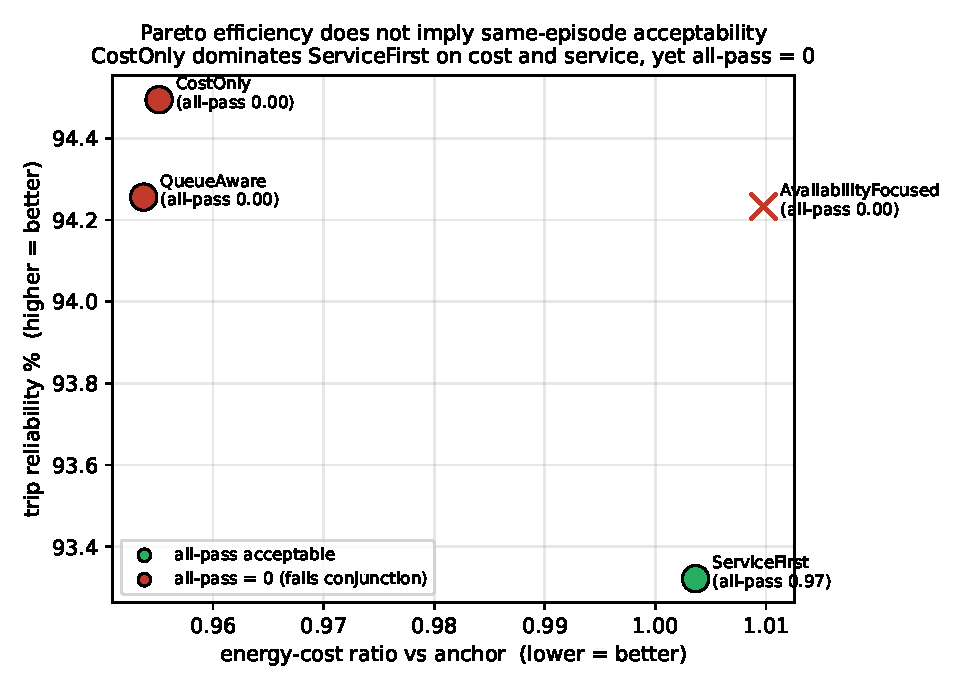
\includegraphics[width=0.62\textwidth]{figures/fig_eq_pareto.pdf}
\caption{Pareto efficiency does not imply same-episode acceptability (full compliance). Each scheduling policy is plotted by energy-cost ratio (lower better) and trip reliability (higher better). The cost/reliability-optimal policies CostOnly and QueueAware (red) score $0\%$ same-episode all-pass, while the only acceptable policy, ServiceFirst (green, $96.7\%$), is dominated on both headline objectives---so the conjunctive screen cannot be recovered from a Pareto front over averaged objectives.}
\label{fig:pareto}
\end{figure}

\paragraph{Neither a weighted optimizer nor a hard constraint escapes the behavioral collapse.} The Pareto plot is a single snapshot; a reader might still ask whether \emph{tuning} a weighted objective, or hard-constraining the optimizer, recovers feasibility. This is the refutation test for clause~(ii) of H1: if \emph{any} weighting of the three objectives yielded a feasible blended optimum at the modeled deviation, that clause would be false. We test both directly over the achievable controller menu (ServiceFirst and ServiceGridWeighted operators $\times$ NoGridAdjustment and GridPeakPenalty, $35\%$ capacity), reading each controller's driver, operator, and grid objective from the simulator together with its same-episode all-pass rate (\figref{fig:optbaseline}). A \emph{weighted-sum optimizer} picks the controller minimising $\alpha J_D+\beta J_O+\gamma J_G$, and we sweep the weights $(\alpha,\beta,\gamma)$ over the whole simplex. At full compliance a good weighting is feasible---the blended optimum's mean all-pass is $0.95$ and the best weighting reaches $1.0$. But at the mildest deviation (severity~1, $\sim$5\%) the blended optimum's all-pass is $0.00$ for \emph{every} weighting on the simplex: no choice of $\alpha,\beta,\gamma$ recovers joint feasibility, because the whole achievable menu has collapsed. The \emph{hard-constrained optimizer} of Eq.~\eqref{eq:optwithin}---minimise $J$ subject to all gates passing---makes the same point from the constraint side: at full compliance it returns a feasible controller (ServiceFirst under GridPeakPenalty), but for severity~$\ge 1$ its feasible set is \emph{empty}, so the constrained problem has no solution in the achievable menu. Tellingly, the best-reliability controller keeps delivering $\sim$95\% trip reliability at every severity while its joint all-pass falls from $1.0$ to $0.0$: the single-metric view stays green while joint deployability fails. A compensatory blend can thus be objective-optimal and infeasible at once, and hard-constraining merely relabels the same collapse as infeasibility---the missing ingredient is not a better objective or solver but the behavioral compliance that keeps the feasible set non-empty. Sweeping the entire weight simplex is the strongest available attempt to falsify clause~(ii); that it fails is why we report H1(ii) as surviving refutation rather than as merely robust.

\begin{figure}[t]
\centering
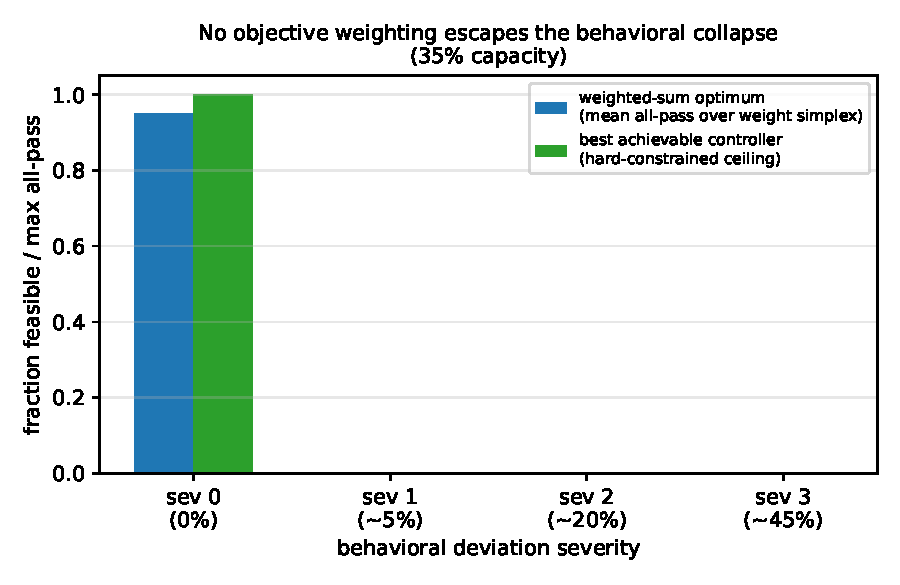
\includegraphics[width=0.62\textwidth]{figures/fig_weighted_optimizer_baseline_20260716.pdf}
\caption{Optimizer baselines cannot escape the behavioral collapse ($35\%$ capacity, achievable controller menu). Blue: the mean same-episode all-pass of the weighted-sum optimum as the weights $(\alpha,\beta,\gamma)$ are swept over the full simplex. Green: the best achievable controller (the ceiling a hard-constrained optimizer could reach). At full compliance a feasible weighting exists; from the mildest deviation onward every weighting's blended optimum is infeasible and the hard-constrained feasible set is empty (no solution to Eq.~\eqref{eq:optwithin}). The collapse is a property of behavior, orthogonal to the objective weighting.}
\label{fig:optbaseline}
\end{figure}

\subsection{Applying the framework to recognized published controllers}\label{sec:published}

The previous result uses our own policy family, so a fair question is whether the screen would reach a different verdict for an \emph{established} controller from the charging-control literature, or whether it simply rejects policies built for the purpose. We therefore apply the framework to two recognized published controllers and report the result at full compliance, where the controller---not driver behavior---is on trial (\tabref{tab:published}). First, we note that the schedulers underlying our own families are themselves canonical: least-laxity-first \cite{dertouzos1989llf} and earliest-deadline-first \cite{liu1973scheduling} are classical real-time scheduling algorithms, and the production ACN adaptive charging scheduler belongs to this deadline-driven family \cite{lee2021adaptive}. We then run two external reference controllers through the gates: (i)~\emph{Earliest-Deadline-First} (EDF) as a recognized deadline scheduler in its own right, and (ii)~\emph{uncoordinated immediate charging}---the universal business-as-usual baseline in which every vehicle charges as soon as a charger is physically free, with no deferral, prioritization, or deadline ordering \cite{clement2010,ma2013}.

The screen produces exactly the conclusion a single-metric evaluation would miss. All three controllers achieve high trip reliability ($91.9$--$95.4\%$ in this $35\%$-capacity, full-compliance cell), the conventional service metric on which each would be judged adequate. Yet the same-episode 14-gate conjunction separates them sharply. EDF, despite $94.6\%$ reliability and passing the operator and grid gates \emph{entirely}, satisfies the joint screen in only $0.20$ of episodes, because it fails the relative critical-service driver gate in $80\%$ of episodes: it is a competent deadline scheduler whose per-episode critical-delivery falls just short of the least-laxity anchor often enough that, conjoined with the other gates, joint feasibility rarely holds. Uncoordinated charging is worse in a different way: at $91.9\%$ reliability and the lowest cost (it passes the charging operator \emph{cost} sub-gate), it nonetheless scores $0.000$ all-pass because immediate charging under constrained capacity produces severe queue congestion (95th-percentile waits two orders of magnitude above the $30$-minute gate) and a degraded load shape, failing the charging operator-queue and grid-shape gates. The framework is therefore not arbitrarily rejecting sophisticated policies: the competent least-laxity-anchored service policy passes (all-pass $1.00$ in this $35\%$ cell, $0.967$ pooled across capacities), a recognized deadline scheduler fails subtly through relative critical service, and the naive baseline fails grossly through congestion---three published or canonical controllers, three different verdicts, each invisible to a reliability-only reading. Supplementary Fig.~\ref{fig:published} contrasts the single reliability metric against the same-episode conjunction for the three controllers.

These controllers span the families a reader is most likely to use. The EDF case directly covers the production ACN adaptive charging algorithm, which is a deadline-driven scheduler of this family \cite{lee2021adaptive}; the uncoordinated case covers the no-control baseline. The remaining mainstream family is price-responsive / valley-seeking control, in which vehicles charge toward low-price or low-aggregate-load windows---the spirit of decentralized cost-minimizing charging \cite{ma2013}. Our CostOnly policy is a deliberately simplified member of this family (it shifts discretionary charging into cheap windows without solving a full load-variance-minimizing valley-fill), and it is already informative: it is Pareto-efficient on cost and reliability yet scores $0.000$ same-episode all-pass (Section~\ref{sec:results}, \figref{fig:pareto}), so the price-responsive family fails the conjunction as well, for a third distinct reason (cost-driven waiting and load-shape stress). We do not implement a full decentralized-optimization controller such as an ADMM or projected-gradient valley-filling scheme; because the screen is a post-hoc evaluation of any controller's realized per-episode trajectories, such schemes can be passed through the same gates without modification, and doing so is a natural extension rather than a change to the method.

\begin{table}[t]
\centering
\caption{Applying the same-episode screen to recognized published controllers (full compliance, 35\% capacity, five seeds). All three reach high trip reliability---the conventional single metric---but the 14-gate same-episode conjunction discriminates sharply: a competent least-laxity-anchored policy passes, the recognized EDF scheduler fails through the relative critical-service driver gate, and the universal uncoordinated baseline fails through queue congestion and load shape.}
\label{tab:published}
\begin{tabular}{lcccccc}
\hline
Controller & Trip reliab. & Driver & Operator & Grid & All-pass & p95 wait (min) \\
\hline
ServiceFirst (least-laxity-anchored) & 95.4\% & 1.00 & 1.00 & 1.00 & \textbf{1.00} & 0 \\
Earliest-Deadline-First (EDF) & 94.6\% & 0.20 & 1.00 & 1.00 & \textbf{0.20} & 0 \\
Uncoordinated immediate charging & 91.9\% & 0.00 & 0.00 & 0.00 & \textbf{0.00} & $\sim$3568 \\
\hline
\end{tabular}
\end{table}

\subsection{Low-deviation behavior collapses same-episode acceptability}

\figref{fig:severity} and \tabref{tab:weeklyseverity} summarize the 20-seed severity curve (three capacities, both grid policies, service-oriented family). Full compliance passes all actor gates in 96.7\% of episodes; the residual failures are grid load-shape trips discussed in Section~\ref{sec:robust}. The severity-1 collapse is not an artifact of the strict 14-way conjunction: it is already present \emph{before} any cross-actor AND. The driver-service gate alone---a single actor---falls to 0.050, and within it the critical-requested-not-delivered criterion fails in $92\%$ of episodes (its mean rising from $0$ to $46$ dropped critical requests against a threshold of $24$); the operator and grid gates alone fall to 0.188 and 0.321, while nine of the fourteen criteria still fail in under $2\%$ of episodes. The degradation is thus concentrated in a few criteria failing hard, not in many gates each failing slightly. The strict same-episode all-pass rate ($1.2\%$) is the aggregate consequence of these single-actor failures, read together with the graded fraction-of-criteria index, which drops to $0.79$ at severity~1 (Section~\ref{sec:robust}); we report all three so the result does not rest on the binary conjunction alone. The actual/operator request-event ratio increases from 0.984 to 1.096 at severity 1 and to 2.164 at severity 3. The severity-0 value is below one because the denominator counts operator recommendations before grid adjustment, while fully compliant drivers follow the grid-adjusted action stream.

\begin{figure}[t]
\centering
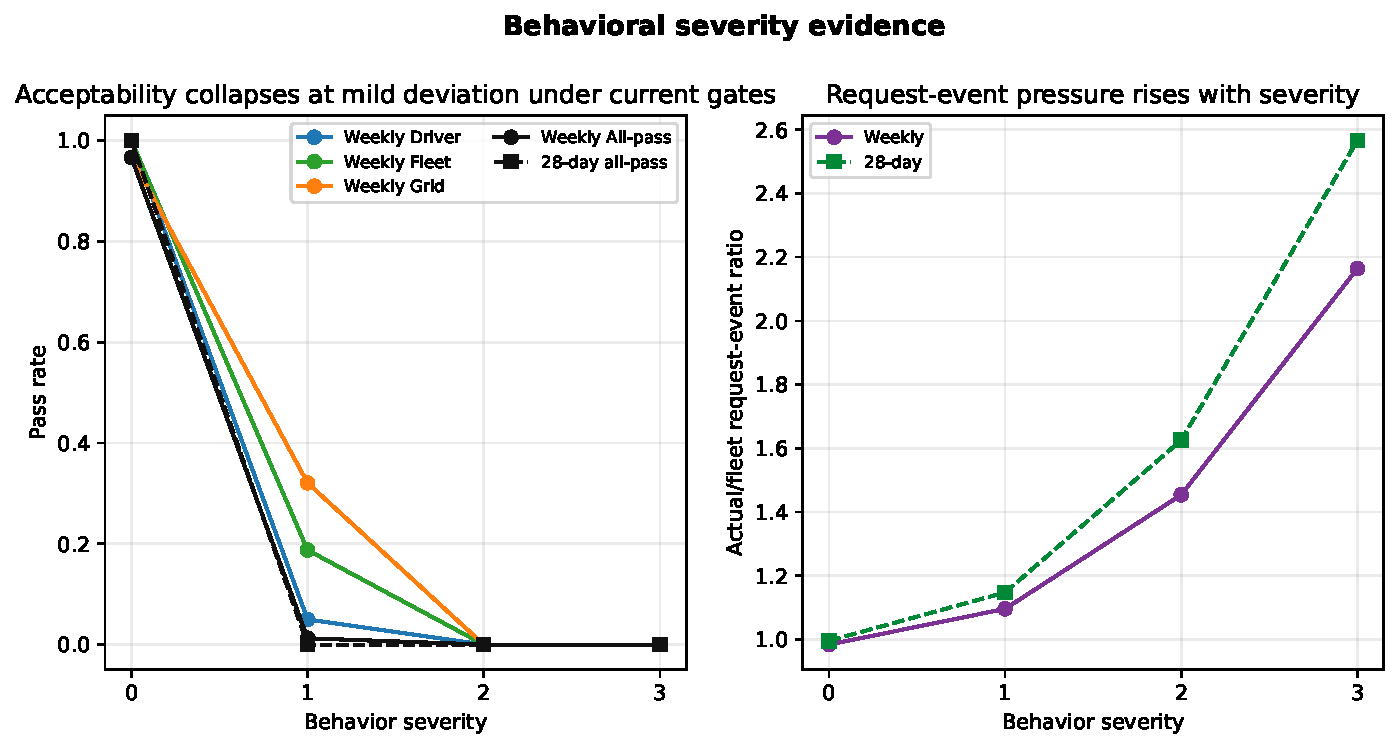
\includegraphics[width=0.72\textwidth]{figures/fig3_behavioral_severity_curve.pdf}
\caption{Behavioral severity curve. The result claim is that request-event pressure rises smoothly with severity, while the same-episode all-pass conjunction fails at severity 1 under the current gates.}
\label{fig:severity}
\end{figure}

\begin{table}[t]
\centering
\caption{Behavioral severity results under the normative gates of Table~\ref{tab:gates} (20-seed expansion: seeds 4541--4560, capacities 20/35/50\%, both grid policies, service-oriented family; 240 episodes per severity). All-pass is a threshold-conditioned indicator; the single-actor and graded-criteria columns (and Section~\ref{sec:robust}) show the degradation is present before the strict conjunction.}
\label{tab:weeklyseverity}
\resizebox{\textwidth}{!}{%
\begin{tabular}{cccccccc}
\hline
Severity & Driver pass & Operator pass & Grid pass & All-pass & Actual/operator events & Delivered ratio & Peak ratio \\
\hline
0 & 1.000 & 1.000 & 0.967 & 0.967 & 0.984 & 1.000 & 0.940 \\
1 & 0.050 & 0.188 & 0.321 & 0.012 & 1.096 & 0.989 & 0.954 \\
2 & 0.000 & 0.000 & 0.000 & 0.000 & 1.454 & 0.964 & 0.971 \\
3 & 0.000 & 0.000 & 0.000 & 0.000 & 2.164 & 0.952 & 0.993 \\
\hline
\end{tabular}%
}
\end{table}

The result indicates a joint-threshold effect under the current actor gates rather than a physical discontinuity in charging service: driver and operator gates bind first, with grid gates increasingly binding. The severity-1 all-pass rate remains near zero across the threshold settings swept in supplementary Supplementary \figref{fig:suppthresh}---tightening the delivered-ratio gate from 0.95 to 0.99 removes 18 of the severity-0 all-pass rows and requiring 1.00 removes 60, yet the severity-1 collapse is unchanged---and Section~\ref{sec:robust} examines this robustness in detail.

This same-episode framing is precisely what distinguishes the screen from scenario-averaged evaluation. If the severity-1 service-oriented metrics are instead averaged across episodes and then checked against the gates---the implicit logic of a scenario-averaged or Pareto-frontier comparison---11 of the 14 gates pass, including the delivered-energy ratio (mean 0.99), peak ratio (0.96), energy-cost ratio (0.99), and all queue metrics, and the policy would be judged broadly acceptable. Yet the same-episode all-pass rate is near zero (1.2\% in the 20-seed weekly sweep): the binding violations (critical requests, 95th-percentile wait, and load shape) fall in \emph{different} episodes, so almost no single episode satisfies all gates at once. A scenario-averaged or marginal-objective evaluation therefore misses the joint failure that the same-episode screen exposes, which is the core value the framework adds beyond average-case or Pareto analysis. \figref{fig:marginaljoint} makes this gap the primary measurement of the paper: panel~(A) is the scenario-averaged dashboard a planner would conventionally read---nine of the fourteen criteria pass in at least $98\%$ of episodes and the mean fraction of criteria passed is $0.79$ ($\approx$11 of 14), so each criterion checked alone looks acceptable---while panel~(B) shows that requiring all fourteen in the \emph{same} episode collapses acceptability to $1.2\%$. The $79\%$-marginal-to-$1.2\%$-joint gap is not a stricter standard applied to the same data; it is the difference between asking whether each constraint is usually met and asking whether they are ever met together, and only the latter is the deployment question.

\begin{figure}[t]
\centering
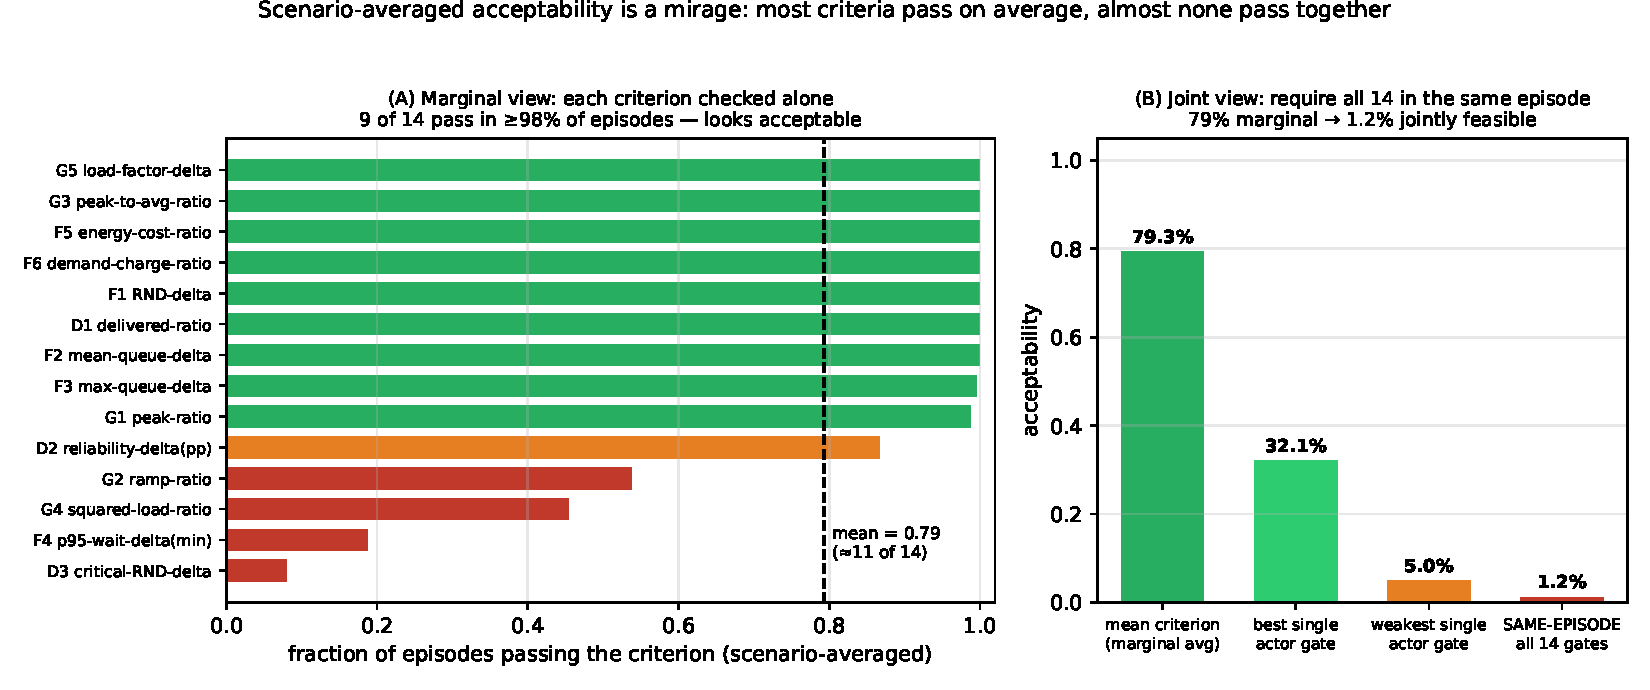
\includegraphics[width=0.82\textwidth]{figures/fig_marginal_vs_joint.pdf}
\caption{Scenario-averaged acceptability is a mirage; same-episode feasibility is the deployment question (severity~1, 20-seed service-oriented family). (A)~Marginal view: each of the fourteen gate criteria scored by the fraction of episodes it passes on its own; nine pass in $\geq98\%$ of episodes and the mean is $0.79$ ($\approx$11 of 14), so a per-criterion dashboard reads as broadly acceptable. (B)~Joint view: the same data under increasingly strict conjunction---mean single criterion ($79\%$), best and weakest single actor gate ($32\%$ and $5\%$), and the same-episode all-fourteen conjunction ($1.2\%$). The collapse from $79\%$ marginal to $1.2\%$ joint is the core quantity the framework measures, because the binding violations fall in different episodes.}
\label{fig:marginaljoint}
\end{figure}

\tabref{tab:marginaljoint} gives the gate-by-gate numbers behind this contrast. Read down the ``scenario-averaged'' column---the fraction of severity-1 episodes in which each criterion passes \emph{on its own}---and the policy looks acceptable: ten of the fourteen criteria pass in at least $87\%$ of episodes and nine in at least $99\%$, so a planner checking criteria one at a time, or against scenario-averaged metrics, would clear it. Only three criteria fall substantially (critical-requested-not-delivered $0.08$, 95th-percentile wait $0.19$, squared-load ratio $0.45$), and even these would typically be read as ``mostly passing.'' The same-episode conjunction in the final row, $0.012$, is the deployment-relevant quantity: because those binding violations land in \emph{different} episodes, almost no single episode satisfies all fourteen at once. The table is the precise, auditable form of \figref{fig:marginaljoint}, and the gap between the column-wise average ($0.79$) and the joint rate ($0.012$) is the framework's central measurement.

\paragraph{The collapse is not an artifact of ANDing many gates.} A natural objection is that requiring \emph{fourteen} criteria at once mechanically forces a low rate, so the collapse is a counting artifact rather than a fact about behavior. It is not. We pre-declare a \emph{minimal} set of three gates---one binding criterion per actor, the same three the diagnostic identifies: critical-requested-not-delivered (driver), 95th-percentile wait (operator), and the load-shape ratio (grid)---and require only those three in the same episode (\figref{fig:minimal}). The minimal three-gate conjunction reproduces the full fourteen-gate all-pass \emph{exactly}---$0.967\rightarrow0.012$ pooled, and $0.975\rightarrow0.000$ at $35\%$---because the eleven non-binding criteria pass at severity~1 and add nothing to the conjunction. Dropping from fourteen gates to three changes the numbers not at all; the collapse is carried entirely by the three binding criteria. Sharper still, the single driver criterion \emph{alone} falls from $1.00$ to $0.05$ pooled ($0.00$ at $35\%$), so no conjunction is needed to see it. Together with the monotonicity argument of Section~\ref{sec:formulation} (adding gates can only lower the rate), this brackets the result from both sides---the collapse is invariant to the gate count, upward and downward---so it is a property of the behavior, not of how many criteria are stacked.

\begin{figure}[t]
\centering
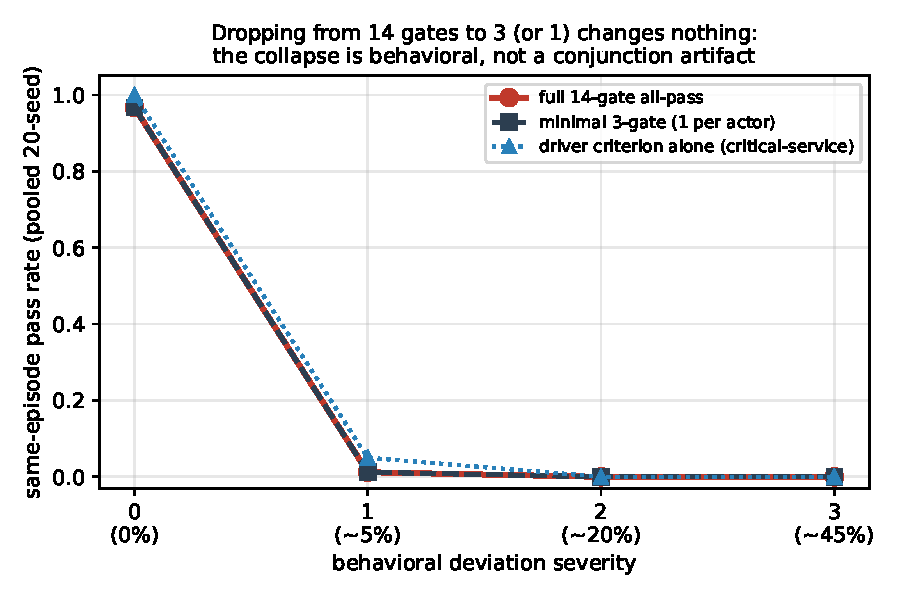
\includegraphics[width=0.6\textwidth]{figures/fig_minimal_gateset_20260716.pdf}
\caption{The collapse is not a fourteen-gate ANDing artifact. Same-episode pass rate (pooled 20-seed factorial) for the full fourteen-gate all-pass (red), a minimal three-gate conjunction using one binding criterion per actor (dark, dashed), and the single driver criterion alone (blue, dotted). The three-gate conjunction reproduces the fourteen-gate rate exactly ($0.967\rightarrow0.012$ at severity~1) because the eleven non-binding gates pass and contribute nothing; the driver criterion alone already falls to $0.05$. Dropping from fourteen gates to three---or to one---does not soften the collapse, so it is behavioral rather than a product of stacking criteria.}
\label{fig:minimal}
\end{figure}

\begin{table}[t]
\centering
\caption{Scenario-averaged (marginal) versus same-episode (joint) acceptability at severity~1, gate by gate (20-seed service-oriented family). The scenario-averaged column is the fraction of episodes in which each criterion passes on its own; the same-episode conjunction (final row) requires all fourteen to hold in the \emph{same} episode. Most criteria pass marginally, yet joint feasibility is near zero because the binding violations fall in different episodes.}
\label{tab:marginaljoint}
\begin{tabular}{llc}
\hline
Actor & Gate criterion & Scenario-averaged pass rate \\
\hline
Driver & Delivered-energy ratio & 1.000 \\
Driver & Reliability delta & 0.867 \\
Driver & Critical requested-not-delivered & \textbf{0.079} \\
Operator & Requested-not-delivered delta & 1.000 \\
Operator & Mean-queue delta & 1.000 \\
Operator & Max-queue delta & 0.996 \\
Operator & 95th-percentile wait delta & \textbf{0.188} \\
Operator & Energy-cost ratio & 1.000 \\
Operator & Demand-charge ratio & 1.000 \\
Grid & Peak ratio & 0.988 \\
Grid & Ramp ratio & \textbf{0.538} \\
Grid & Peak-to-average ratio & 1.000 \\
Grid & Squared-load ratio & \textbf{0.454} \\
Grid & Load-factor delta & 1.000 \\
\hline
\multicolumn{2}{l}{\emph{Mean of the fourteen marginal pass rates}} & 0.793 \\
\multicolumn{2}{l}{\textbf{Same-episode all-pass (14-gate conjunction)}} & \textbf{0.012} \\
\hline
\end{tabular}
\end{table}

The behavioral effect is request-event churn, not higher energy demand. A demanded-kWh trace over the targeted 28-day cases balances to numerical tolerance (Eq.~\eqref{eq:ledger}) and shows noncompliant vehicles re-entering the request pipeline at additional timesteps via the reserve and cheap-window rule, even when target/deadline-deficit demand is unchanged or lower: aggregate request-event counts rise to $2.349\times$ severity~0 at severity~3 while simulator demanded kWh \emph{falls} to $0.917\times$. Supplementary Fig.~\ref{fig:suppcons} breaks the churn down by behavior type (price-sensitive and SoC-compliance churn most) and reports a request-ID conservation audit with zero count residual. The mechanism is therefore request-event pressure and service-accounting stress, not energy amplification. This decomposition is mediated by the simulator's ledger (a different demand-accounting structure could partition the same behavior differently); what is architecture-independent is that the failure is driven by request timing and frequency, not total energy delivered, which falls slightly.

\paragraph{Targeted 28-day confirmation.} Supplementary Table~\ref{tab:target28} reports the targeted 28-day confirmation at 35\% capacity (a separate five-seed, 672 h run). The longer horizon is a targeted check, not a full-capacity confirmation. In this five-seed 35\% capacity cell, all-pass falls from 100.0\% at severity 0 to 0.0\% at severity 1; the slightly higher severity-0 value than the 20-seed weekly mean reflects the smaller seed set and the single capacity. Request-event pressure rises smoothly from 0.995 at severity 0 to 2.566 at severity 3.

Two of the fourteen gates use absolute event-count thresholds (the critical and total requested-not-delivered deltas), which are extensive and therefore grow with horizon; scoring the 672 h run against the per-week thresholds makes those two gates effectively four times stricter than in the weekly screen, so the 28-day result above is best read as a conservative longer-horizon stress check. To separate the behavioral effect from this horizon-scaling, we re-scored the same 28-day episodes with horizon-fair count thresholds, scaling the two count gates by $672/168=4$ (critical requested-not-delivered delta from $24$ to $96$, requested-not-delivered delta from $117$ to $468$) while leaving the twelve intensive ratio, percentile, and load-shape gates unchanged. The severity-1 collapse is unchanged: all-pass remains $1.000$ at severity~0 and $0.000$ at severity~1 under the horizon-fair thresholds, so the 28-day failure is not an artifact of applying weekly count thresholds over the longer horizon. (A recomputation of the gates from the recorded per-episode metrics reproduces the engine's original all-pass labels exactly.)

The 28-day confirmation is targeted rather than exhaustive because it uses 35\% capacity only. It is best interpreted as a longer-horizon check of one binding capacity cell, with capacity generalization left to future expanded runs.

\subsection{Where it fails, which gate binds, and which behavior drives it}\label{sec:diagnostic}

The diagnostic value of the framework is not the pooled $1.2\%$ figure but the disaggregated answer to \emph{where} feasibility fails, \emph{which} constraint binds first, and \emph{which} behavior is the binding cause. \figref{fig:eqdiag} reports all three, and each carries a different operational implication.

\paragraph{Where: the collapse is uniform across capacity, so it is not an infrastructure problem.} Disaggregating all-pass by charger capacity (\figref{fig:eqdiag}A) shows that severity-1 feasibility is near zero at \emph{every} capacity---$0.038$, $0.000$, and $0.000$ at $20\%$, $35\%$, and $50\%$---and that at full compliance higher capacity is if anything slightly \emph{worse} ($0.988\to0.938$), because more simultaneous charging worsens the grid load-shape sub-gate. Adding chargers therefore does not recover feasibility; it raises the full-compliance plateau marginally and lowers it at the top end, but the severity-1 cliff is present regardless. This is the first concrete deployment message: where the binding constraint is compliance, infrastructure expansion is the wrong lever.

\paragraph{Which gate: the driver-service constraint binds first.} Across capacities at severity~1 (\figref{fig:eqdiag}B), the driver-service gate is the lowest-passing actor constraint---$0.15$ at $20\%$ and $0.00$ at $35\%$ and $50\%$---ahead of the operator ($0.11$--$0.25$) and grid ($0.15$--$0.66$). The grid gate is actually the \emph{healthiest} at low capacity ($0.66$ at $20\%$) and degrades as capacity rises, the opposite of the driver gate. So the leading edge of infeasibility is the driver's own service guarantee: behavioral deviation first breaks the constraint of the very actor whose behavior it is.

\paragraph{Which behavior: recommendation-override request churn, not inattention.} Decomposing by the five non-compliance behavior types under full-strength deviation (\figref{fig:eqdiag}C) localizes the cause. The mild \emph{inattention} behaviors, which merely drop occasional requests (request-churn ratio $\approx0.95$), only partially degrade feasibility ($0.83$ at $2.5\%$ and $0.53$ at $5\%$ inattention) and bind the grid gate. By contrast, the \emph{recommendation-override} behaviors---urgency, reserve-seeking, SoC-anxiety, price-sensitivity, and SoC-plus-queue---collapse feasibility to $0.00$ and bind the driver gate, and they do so with request-churn ratios of $1.3$ to $9.5\times$: a price-sensitive or SoC-anxious driver re-enters the request pipeline many times more often than recommended. The binding cause is therefore not how \emph{often} drivers deviate but \emph{what} they do when they deviate---recommendation-override reserve and price-driven charging that multiplies request events---and the operational implication is specific: an effective intervention must suppress recommendation-override churn (e.g.\ a compliance incentive aimed at reserve- and price-driven overriding), whereas reducing benign inattention would not recover feasibility.

\begin{figure}[t]
\centering
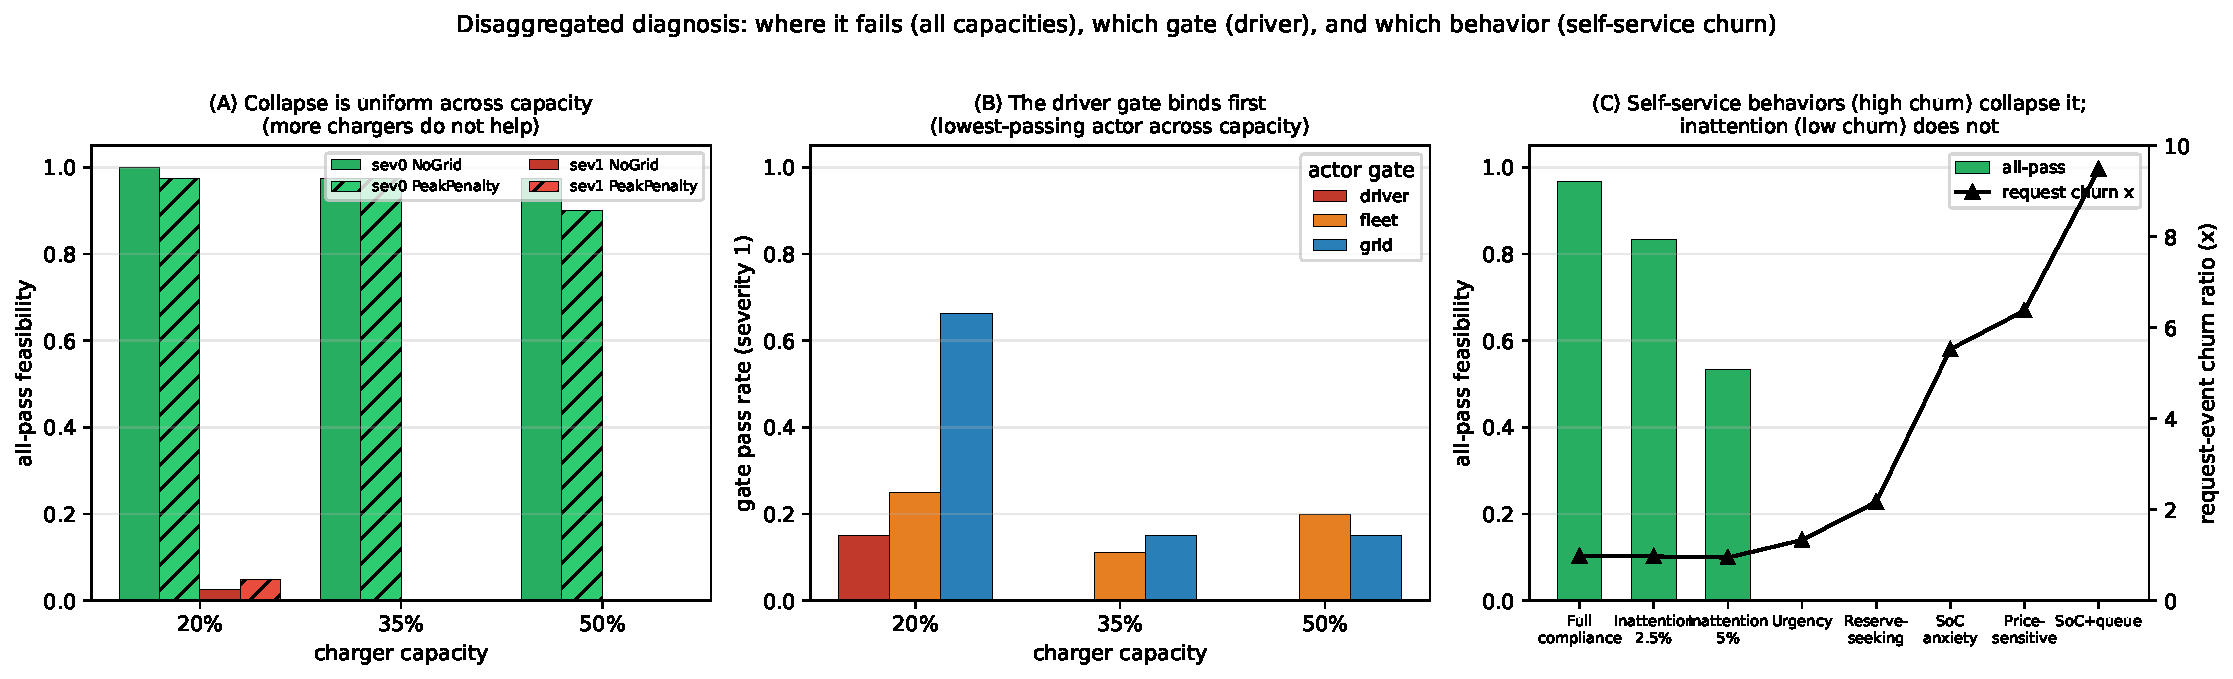
\includegraphics[width=0.88\textwidth]{figures/fig_eq_diagnostic.pdf}
\caption{Disaggregated diagnosis. (A)~All-pass feasibility by charger capacity and grid policy at full compliance (green) and severity~1 (red): the collapse is uniform across capacity, so infrastructure is not the lever. (B)~Actor-gate pass rates by capacity at severity~1: the driver-service gate binds first (lowest-passing) across capacities, while the grid gate is healthiest at low capacity. (C)~All-pass (bars) and request-event churn ratio (line) by behavior type: recommendation-override behaviors (high churn, $1.3$--$9.5\times$) collapse feasibility and bind the driver gate, whereas mild inattention (low churn) does not.}
\label{fig:eqdiag}
\end{figure}

\paragraph{The corrective lever works by the diagnosed mechanism.} If the binding cause is the recommendation-override override \emph{motive} rather than the deviation rate itself, then suppressing that motive---what a service guarantee or congestion-aware override charge is designed to do (Section~\ref{sec:discussion})---should recover feasibility even at an unchanged deviation rate. We test this directly in the engine. Holding the deviation rate fixed, we replace the recommendation-override reserve/price override with a behaviorally benign deviation (the vehicle abstains rather than churning the request pipeline) and re-score the gates (\figref{fig:instrument}). The contrast is sharp: recommendation-override deviation collapses same-episode all-pass to $0.00$ already at a $2.5\%$ rate, whereas benign deviation at the \emph{same} $2.5\%$ rate holds feasibility at $0.60$ (95\% bootstrap CI $[0.45,0.75]$); by $5\%$ even benign deviation has largely collapsed ($0.05$). This is a mechanism-targeting counterfactual, not a claim that any specific real instrument was validated: it confirms the causal claim of the diagnosis---the override motive, not the rate, triggers the immediate collapse---and shows that an instrument acting on that motive recovers most feasibility at low deviation. It also shows the two levers are \emph{complementary}: by $5\%$ benign deviation retains only $0.05$ and by $10\%$ fails entirely ($0.00$), so motive-targeting instruments must be paired with raising compliance (keeping the rate below the ${\sim}1.5\%$ cliff of Section~\ref{sec:robust}), neither alone being sufficient at high deviation.

\begin{figure}[t]
\centering
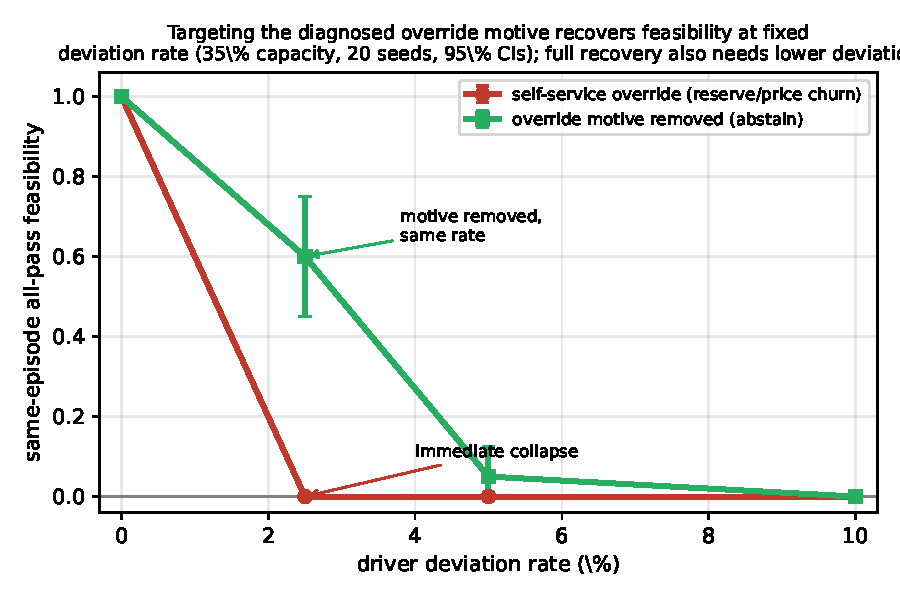
\includegraphics[width=0.62\textwidth]{figures/fig_instrument_counterfactual.pdf}
\caption{Mechanism-targeting counterfactual (35\% capacity, both grid policies, 20 seeds, 95\% bootstrap CIs). Same-episode all-pass versus the driver deviation \emph{rate} for two deviation \emph{types}: recommendation-override override (reserve/price churn, red) collapses to zero already at $2.5\%$, whereas removing the override motive (benign abstention, green)---what service guarantees and override pricing target---holds feasibility at $0.60$ at $2.5\%$ but only $0.05$ at $5\%$. Targeting the diagnosed motive recovers feasibility at a fixed rate, but full recovery also requires lower deviation, so the instruments and the compliance incentive are complementary.}
\label{fig:instrument}
\end{figure}

\paragraph{Information integrity is a second, equally-fragile compliance axis.} The results so far model \emph{action}-level non-compliance---drivers report their true needs but override the recommended action. A distinct failure mode is \emph{information}-level non-compliance: drivers report \emph{untruthfully} to game a scarce shared resource. We test this by letting a share of drivers claim false urgency (misreport an imminent deadline) so the least-laxity scheduler prioritizes them, while the gates are scored against \emph{true} service and drivers otherwise fully comply. The scheduler re-implementation used for this test reproduces the truthful baseline \emph{exactly} at a negligible misreport share (all-pass $1.00$ at both $0\%$ and $0.1\%$), so any degradation is a genuine information-integrity effect rather than an implementation artifact. Under strategic misreporting, feasibility collapses on essentially the \emph{same} cliff as action non-compliance (\figref{fig:infointegrity}): same-episode all-pass falls to $0.25$ at a $2\%$ misreport share and $0.05$ at $5\%$, with the driver-service gate binding first because false-urgency queue-jumpers displace the truly-urgent, whose critical charges are then missed. Truthful information sharing is therefore not a bonus over the baseline but a \emph{maintained assumption} whose violation is a second, upstream compliance failure---so deployable managed charging needs \emph{both} action-compliance incentives (Section~\ref{sec:game}) and information-integrity mechanisms, e.g.\ the departure-time and minimum-SoC elicitation of Section~\ref{sec:discussion} made incentive-compatible. This is a strategic worst case (persistent, maximal false urgency); milder misreporting would degrade feasibility more gradually.

\begin{figure}[t]
\centering
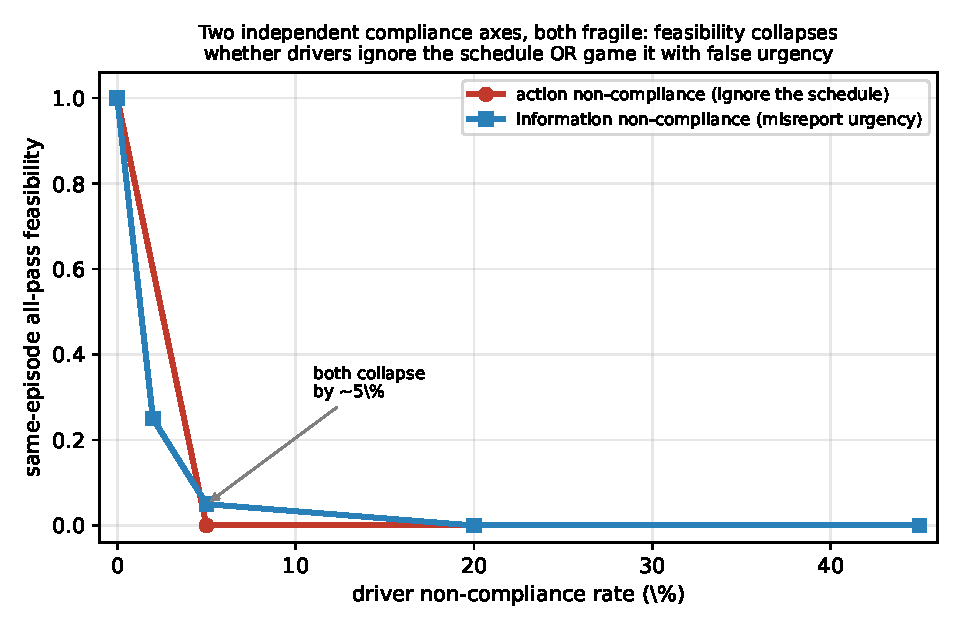
\includegraphics[width=0.62\textwidth]{figures/fig_information_integrity.pdf}
\caption{Two independent compliance axes, both fragile (workplace, 20-seed, 35\% capacity). Same-episode all-pass versus the driver non-compliance rate for \emph{action} non-compliance (drivers ignore the recommended action, red) and \emph{information} non-compliance (drivers misreport urgency to the scheduler while gates score true service, blue). Feasibility collapses by roughly $5\%$ non-compliance on either axis; the information axis is validated to reproduce the truthful baseline at a negligible misreport share. Managed charging thus requires both action compliance and information integrity.}
\label{fig:infointegrity}
\end{figure}

\subsection{The collapse is multi-actor, broad-based, and weight-independent}\label{sec:robust}

A legitimate concern is that the same-episode all-pass collapse is an artifact of ANDing many fragile binary criteria. We test this with a 20-seed dataset for the service-oriented family (240 episodes per severity: seeds 4541--4560, three capacities, two grid policies, two service operator policies) through seven checks, summarized in Table~\ref{tab:robustsummary}; the collapse survives all of them. The expansion also refines the headline: under full compliance all-pass is 0.967, not exactly 1.000 (the grid load-shape gate trips on a minority of seeds, and severity-0 all-pass declines with capacity, 0.988/0.975/0.938 at 20/35/50\%; Supplementary Table~\ref{tab:seedcap}). The severity-0-versus-1 collapse is confirmed by non-overlapping bootstrap intervals (0.967, $[0.942, 0.988]$ versus 0.012, $[0.000, 0.029]$; 10{,}000 resamples of the episode-level indicators, the episode being the independent seed--capacity--policy draw).

\begin{table}[t]
\centering
\caption{Robustness of the severity-1 same-episode all-pass collapse across seven checks (20-seed service-oriented family unless noted). The collapse is broad-based, survives softer aggregation and a wide threshold envelope, and is insensitive to deviation placement, preference form, and scheduler choice.}
\label{tab:robustsummary}
\begin{tabular}{lll}
\hline
Check & What is varied & Severity-1 result \\
\hline
1. Binding criteria & which of 14 gates fail & 4 criteria, all 3 actors (0.92/0.81/0.55/0.46); 9 fail $<$0.02 \\
2. Aggregation logic & AND $\to$ $\geq$1 actor; graded & driver-alone 0.05; $\geq$1-actor 0.43; graded frac.\ 0.79 \\
3. Threshold envelope & all 14 margins scaled & $<$0.07 up to $1.5\times$; clears 0.5 only at $3\times$ \\
4. Single-gate loosen & one cut-point $\times3$ & $\leq$0.054 (no single gate responsible) \\
5. Deviation placement & low- vs high-laxity & 0.000 in both \\
6. Preference form & 8 coefficient variants & 0.000 for every variant \\
7. Scheduler & EDF; oracle selection & EDF 0.20$\to$0; best single 0.017, oracle 0.050 \\
\hline
\end{tabular}
\end{table}

\emph{Which criteria bind} (\figref{fig:robust}A): the collapse is broad-based, with four criteria across all three actors failing---critical-requested-not-delivered (driver, 0.92), 95th-percentile wait (operator, 0.81), squared-load ratio (grid, 0.55), and ramp ratio (grid, 0.46)---while nine criteria fail in under 2\% of episodes; the deliberately tight reliability-delta gate fails in only 0.13 and is not the driver. \emph{Softer aggregation} (\figref{fig:robust}B) shows the degradation before any three-actor AND: the driver gate alone falls to 0.050 and the ``at least one actor'' rate to 0.433, while the graded fraction of criteria passed declines from 1.00 to 0.79/0.61/0.56 at severities 1--3. We therefore report the graded index alongside the binary indicator and do not read the transition as a physical cliff.

The two load-bearing gates have independently defensible thresholds: the critical-not-delivered cut-point ($24$ events per $168$-h week, $\approx3.4$/day) is exceeded roughly twofold at severity~1 (mean 46), and the conventional 30-minute 95th-percentile-wait target by about $1.6\times$ (mean 49), so both binding violations overshoot defensible cut-points rather than sitting at the margin. A global threshold-slack sweep (Supplementary Table~\ref{tab:envelope}) shows severity-1 all-pass staying below 0.07 until every gate is loosened $1.5\times$ and clearing 0.5 only at $3\times$, while loosening any single criterion threefold recovers at most 0.054---so the collapse is not undone by re-tuning one or two thresholds.

On the behavioral side the collapse is insensitive to deviation \emph{placement}---0.000 whether the 5\% deviation is concentrated in low-laxity (the realistic case \cite{alexeenko2023pilot}) or high-laxity vehicles, the driver-service gate binding wherever deviation falls---and to the preference \emph{functional form}, with same-episode all-pass 0.000 across eight coefficient variants of Eq.~\eqref{eq:severitypref} (base, all-equal, reversed, reserve-dropped, SoC-dominated, $\pm50\%$). We note that the coefficient magnitudes (e.g.\ the $26{:}1$ critical-to-laxity ratio) are author-chosen, not calibrated; the ablation bounds but does not validate them, and the citations in Section~\ref{sec:design} ground the preference's \emph{term structure}, not its additive-logit \emph{functional form}, whose behavioral validity remains an open empirical question. This insensitivity to preference form, across both the five behavior types and the eight coefficient variants, justifies collapsing behavior to the scalar deviation index $d$ used in the game of Section~\ref{sec:game}.

On the scheduler side the threshold is scheduler-independent. Earliest-Deadline-First (EDF---the canonical deadline rule and the family of the ACN adaptive scheduler \cite{lee2021adaptive}) collapses identically, its feasibility falling from $0.20$ at full compliance to $0.00$ by $2.5\%$ deviation: scheduler quality sets the full-compliance \emph{level} (0.967 for LeastLaxity-anchored ServiceFirst versus 0.20 for the weaker EDF) while behavioral compliance sets the \emph{threshold}. An oracle counterfactual sharpens this and doubles as a refutation test of clause~(i) of H1---scheduler-invariance (\figref{fig:oracle}): a per-episode hindsight-optimal scheduler is the strongest chance to \emph{break} the claim that no scheduler recovers feasibility, so if it succeeded, H1(i) would be false. Under the standard managed-charging intervention model---a scheduler allocates power and queue order over the realized request stream but cannot coerce a critical request, pre-empt declined energy, or see the future beyond the deadline/laxity signal---the best single deployable scheduler reaches only $0.017$ all-pass at severity~1, and a per-episode hindsight-optimal oracle (an upper bound no real controller can exceed) only $0.050$ ($[0.000, 0.117]$), entirely at the lowest 20\% capacity. The reason is structural (Section~\ref{sec:diagnostic}): the binding gate is the critical-requested-not-delivered driver guarantee, set by whether deviating vehicles depart from their recommended critical-service schedule---an action in the driver's choice set, not the scheduler's. The infeasibility is therefore inherent to the deviation, not the scheduler, which is exactly why the lever is a compliance incentive that reshapes the request stream rather than a better allocation of a broken one. Clause~(i) of H1 thus survives a test built to refute it---an upper-bound scheduler with every chance to succeed---rather than merely a robustness perturbation.

\begin{figure}[t]
\centering
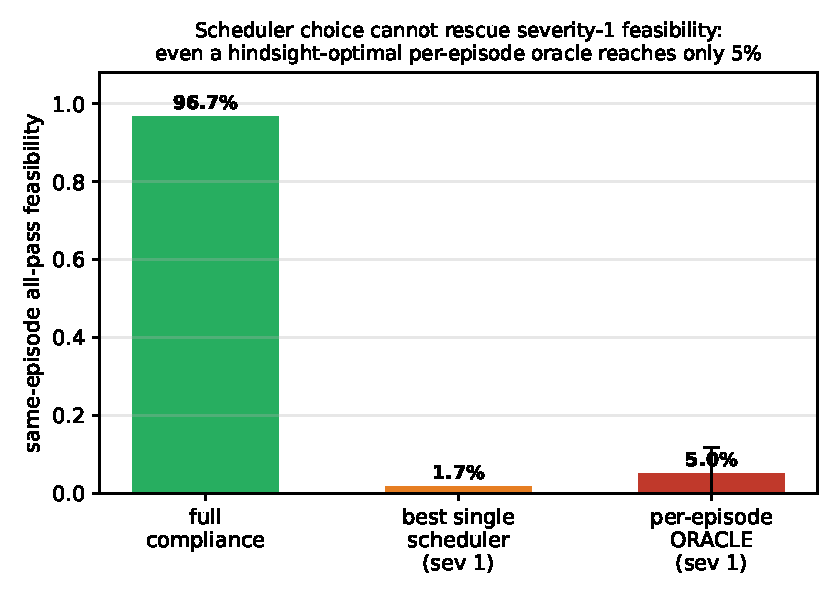
\includegraphics[width=0.62\textwidth]{figures/fig_oracle_scheduler.pdf}
\caption{Oracle scheduler-selection counterfactual at severity~1. Same-episode all-pass under full compliance ($0.967$) versus the best single deployable scheduler ($0.017$) and a per-episode oracle that assigns each episode its best-passing scheduler ($0.050$; error bar is the 95\% episode-bootstrap interval). Even hindsight-optimal scheduler choice cannot recover feasibility, because the binding gate is set by the driver's request behavior, outside the scheduler's action space.}
\label{fig:oracle}
\end{figure}

\begin{figure}[t]
\centering
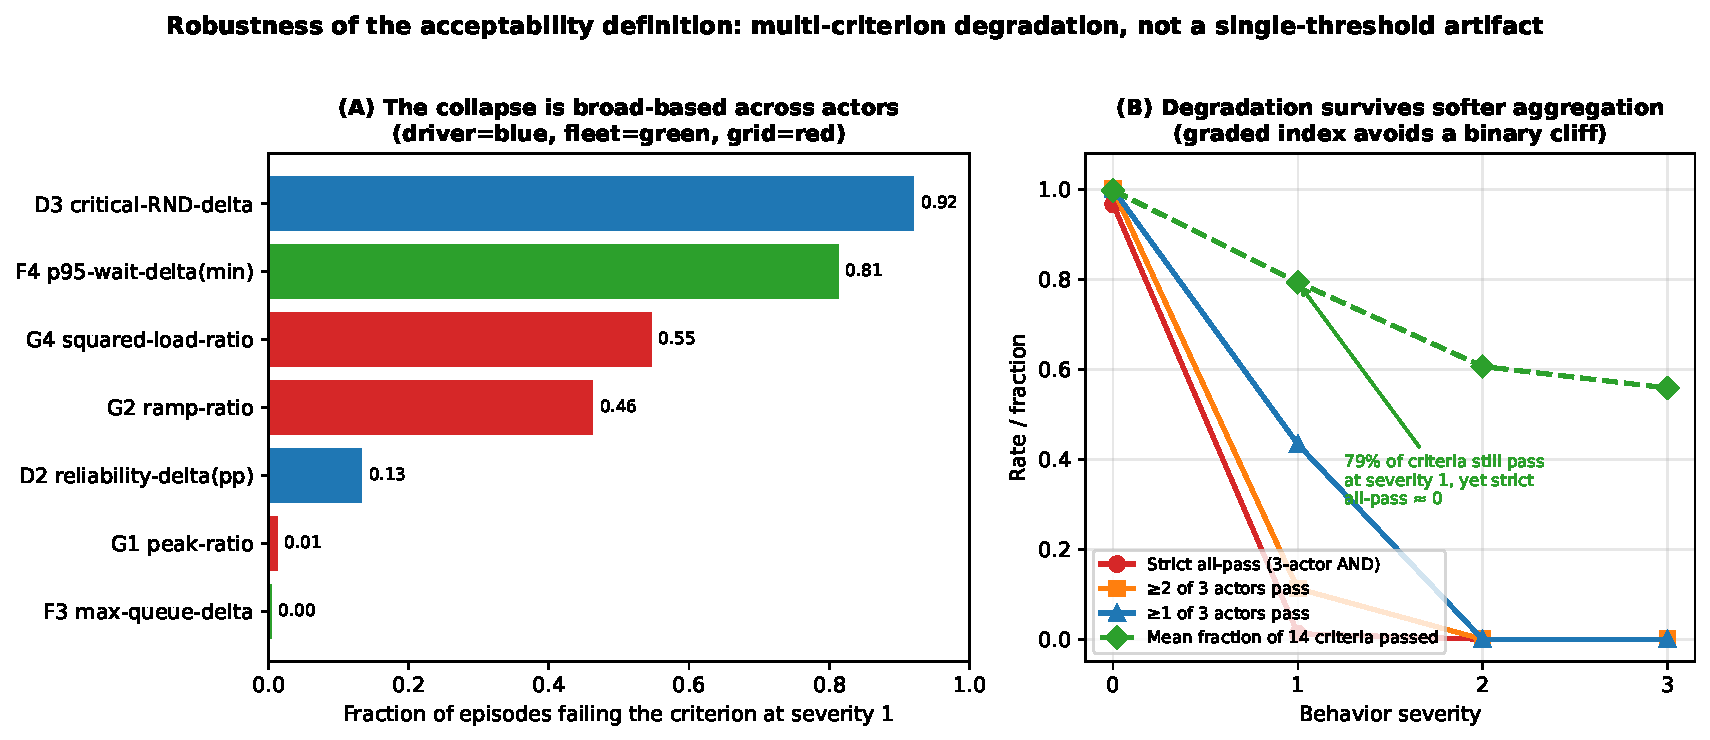
\includegraphics[width=0.82\textwidth]{figures/fig_robustness_acceptability.pdf}
\caption{Robustness of the acceptability definition. (A)~Fraction of severity-1 episodes failing each binding sub-criterion, coloured by actor; the collapse is driven by four distinct criteria across all three actors, not a single tight gate. (B)~Acceptability rate under alternative aggregation logics and the graded fraction-of-criteria index; the degradation survives softer aggregation, while the graded index ($\approx0.79$ of criteria still passing at severity~1) avoids overstating a binary cliff. Twenty-seed service-oriented family.}
\label{fig:robust}
\end{figure}

Two further checks confirm the collapse is not a single-policy or single-metric artifact. The dominant failure pattern is multi-actor: across the 300-row weekly matrix, driver--operator--grid failure accounts for 209 rows versus only 5 single-actor failures (Supplementary Fig.~\ref{fig:failure}). And the result does not depend on the ServiceGridWeighted comparator's integer weights---a six-variant coefficient ablation (Supplementary Material~\ref{sec:supp}) leaves all-pass at 1.00 (severity~0) and 0.00 (severity~1) for every variant, a consequence of the eligibility-based dominance of Section~\ref{sec:formulation}.

\subsection{Grid-side control trades off peaks but does not rescue acceptability}

Having established that actor-gate failure is driven mainly by behavioral request churn, we next ask whether the resulting charging profiles also create interpretable distribution-system stress signals. Supplementary Fig.~\ref{fig:gridtradeoff} compares NoGridAdjustment and GridPeakPenalty. In the targeted 28-day confirmation, GridPeakPenalty reduces the mean peak ratio at severity~1 relative to NoGridAdjustment in several service-oriented groups, but all-pass remains 0.0\%. This means the grid layer can improve selected grid stress metrics without correcting driver and operator acceptability failures. The result supports a trade-off claim, not a rescue claim.


\paragraph{IEEE-33 feeder stress screen.} As an external grid-side lens---not part of the all-pass gate definition and not a site-specific interconnection study---we map each policy's charging profile onto the Baran--Wu IEEE-33 benchmark feeder \cite{baran1989,thurner2018,pandapowerdoc}. Across 900 feeder cases the interpretable policy signals are EV-off-relative deltas: a mean substation-peak delta of $173.8$ kW (range $87.3$--$310.9$), a mean maximum line-loading delta of $3.59$ percentage points, and a mean losses delta of $1718.8$ kWh/week (Supplementary Fig.~\ref{fig:ieee33}). These three metrics, not feeder voltage, carry the grid signal: on this benchmark feeder voltage remains base-load-determined and EV-policy-insensitive, so we do not draw conclusions from it. The grid acceptability gate is governed instead by the load-shape sub-gate: the squared-load and ramp criteria fail in $0.55$ and $0.46$ of severity-1 episodes while the peak-ratio criterion rarely binds ($0.01$), so the grid actor is exercised through load-shape stress.

\subsection{Generalization across charging ecologies: the binding actor is context-dependent}\label{sec:ecology}

The framework above is demonstrated on workplace/campus charging---the setting where a charging operator, long-dwell slack, and shared constrained capacity coexist. Multi-unit-dwelling (apartment) charging shares exactly this structure: residents' vehicles compete for a small shared charger pool managed by a building or charge-point operator, so all three actors and the fourteen gates apply unchanged. We therefore re-run the \emph{identical} framework on a second, data-grounded scenario---a Korean apartment archetype calibrated to multi-unit-dwelling statistics (mean $579$ households per complex, $2.48$ chargers per $100$ households, and $40.5\%$ of complexes with more EVs than chargers)---which shifts the temporal context from morning arrivals and ${\sim}6.6$ h dwells to evening arrivals and overnight (${\sim}12$--$14$ h) dwells. This is a scenario stress test, not an empirical validation of apartment behavior: the workplace case remains the calibrated anchor, the behavioral severity layer is the same model-assumed structure, and run-to-run variation across 20-seed replicates is ${\pm}0.05$, so we report the qualitative trajectory rather than exact decimals.

Three findings follow (\figref{fig:apartment}). First, the same-episode collapse is \emph{universal}: in both ecologies all-pass falls from near one under full compliance to near zero under behavioral deviation, so compliance is the binding fragility regardless of setting. Second, the binding actor is \emph{context-dependent}. Workplace charging has little slack and no buffer: at the severity-1 cliff the driver, charging operator, and grid gates fail together (all ${\approx}0.00$). Apartment charging fails in a \emph{sequence}---at severity~1 the operator queue/waiting gate breaks first ($0.08$, driven by the real charger scarcity), the driver gate \emph{relaxes} ($0.28$, because the large overnight slack makes per-vehicle service easy to meet even under deviation), and the grid gate is still healthy ($0.80$). Third---answering the natural objection that overnight residential charging should stress the grid \emph{more}---the apartment grid benefit is \emph{compliance-contingent}. Under managed charging the overnight slack lets the operator spread the load flat (peak-to-average ${\approx}2.6$ versus ${\approx}4.3$ for workplace), so at high compliance the grid is the \emph{least}-stressed actor; but this benefit decays as residents override the recommendation, the grid gate eroding monotonically from $0.98$ at full compliance to $0.80$, $0.38$, and $0.00$ at severities~1--3 (\figref{fig:apartment}A). The classic evening-peak grid stress is therefore a property of \emph{uncoordinated} (or heavily non-compliant) charging, not of managed apartment charging per se, and it re-emerges precisely as compliance fails.

The unified message is that compliance is the binding constraint in every ecology, but it fails through a different actor: driver service in workplace charging, shared-charger capacity in apartment charging, with the apartment grid benefit itself contingent on compliance. For deployment this is actionable: the apartment EV challenge is first a charger-\emph{provisioning} problem (the operator gate), and the coordination that keeps the grid benign is only as durable as the compliance that sustains it.

\begin{figure}[t]
\centering
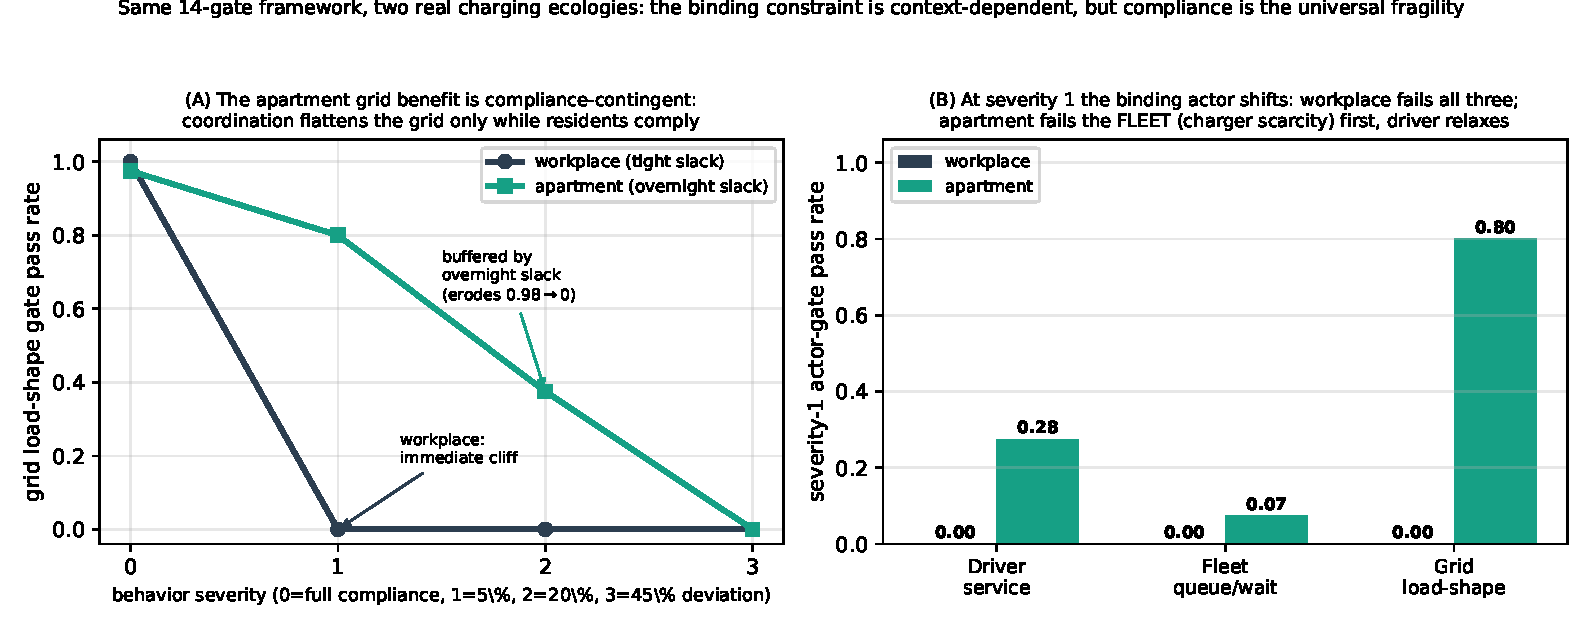
\includegraphics[width=0.99\textwidth]{figures/fig_apartment_vs_workplace.pdf}
\caption{The same 14-gate framework applied to two real charging ecologies (20-seed, 35\% capacity): workplace/campus (ACN-calibrated; morning arrivals, tight slack) versus a Korean apartment/multi-unit-dwelling archetype (overnight arrivals, scarce shared chargers). (A)~Grid load-shape gate versus behavior severity: the workplace grid fails at the severity-1 cliff, whereas the apartment grid is buffered by overnight slack and erodes only gradually ($0.98\to0.80\to0.38\to0.00$)---so the coordination-driven grid benefit is compliance-contingent, not free. (B)~Per-actor gates at severity~1: workplace fails all three actors at once, while apartment fails the charging operator (shared-charger queue) gate first as the driver gate relaxes. The binding stakeholder is context-dependent, but compliance is the universal fragility.}
\label{fig:apartment}
\end{figure}


\section{Mechanism analysis: a congestion-game model of compliance and incentives}\label{sec:game}

The diagnostic result---that small behavioral deviation drives same-episode all-pass
acceptability to near zero---raises the constructive question this section answers:
\emph{is there an operating point at which drivers, charging operator, and grid are simultaneously
acceptable, and what does it cost to reach it?} We show that (i) a calibrated
\emph{congestion-game} representation can place the low-deviation collapse at the
no-incentive compliance equilibrium, rather than treating it only as an exogenous stress
setting; (ii) a cooperative bargaining target provides a transparent reference point for
joint driver, charging operator, and grid utility; and (iii) a bounded Pigouvian-style compliance
incentive, chosen by the operator as a Stackelberg leader, moves the induced equilibrium
into the jointly acceptable region within the calibrated model.

We are explicit about what this layer adds. We do \emph{not} use the game to re-establish the collapse---that is the empirical result of Section~\ref{sec:results}. The game adds three things the simulator alone does not: an \emph{equilibrium explanation} (it endogenizes the deviation level, accounting for why deviation concentrates near $5\%$ as the unique stable Nash equilibrium of a free-riding aggregative game with a congestion externality rather than an exogenous stress setting); a \emph{mechanism-design characterization} of the lever (a Pigouvian-style internalization of the congestion externality---the right \emph{kind} of intervention, not merely ``less deviation helps''); and a \emph{welfare layer} (a Nash-bargaining target and a price of anarchy). It is a complementary explanatory layer, not a re-derivation.

This layer is deliberately subordinate to the screening result and interpretive, not empirical: the game is not estimated from observed strategic choices, its utilities are normative, and $\sigma$ is in normalised utility units. The recovery separates into two mappings we keep distinct: the \emph{physical} mapping from deviation $d$ to acceptability is simulator-validated (every all-pass$(d)$ is a real simulator output), while the \emph{behavioral} mapping from incentive $\sigma$ to lower deviation is a calibrated model assumption. We therefore claim only the conditional---\emph{if} an incentive reduces deviation to $d$, acceptability recovers accordingly---and treat whether an incentive elicits that compliance as a design hypothesis for field validation.

\subsection{Driver compliance as an aggregative game with a congestion externality}

A coordinated charging schedule---drivers accepting the charging operator's recommended deferrals
rather than recommendation-override---produces a shared public good: an uncongested charging queue
and a healthy feeder load shape. The marginal private benefit of complying \emph{falls}
as more drivers comply, because a healthy system can absorb one additional defection:
each driver is then tempted to free-ride by charging immediately or reserve-seeking. Let
$\rho\in[0,1]$ be the aggregate compliance rate and let driver $i$ comply iff
\begin{equation}
\sigma + \beta\,(1-\rho) \;\ge\; \kappa_i,
\label{eq:driverrule}
\end{equation}
where $\sigma\ge 0$ is an operator-paid compliance incentive, $\beta>0$ scales the
congestion externality $(1-\rho)$ that makes complying privately worthwhile, and
$\kappa_i$ is driver $i$'s heterogeneous private compliance cost (higher for low-slack,
inflexible drivers, who deviate first). With $\kappa_i\sim\mathrm{Logistic}(\mu,s)$ the
compliance rate is the fixed point of the aggregative best-response map
\begin{equation}
\rho \;=\; \Phi(\rho;\sigma) \;=\; F_\kappa\!\big(\sigma + \beta(1-\rho)\big),
\qquad F_\kappa(x)=\big[1+e^{-(x-\mu)/s}\big]^{-1}.
\label{eq:fixedpoint}
\end{equation}
Because $\Phi$ is strictly decreasing in $\rho$, the map $g(\rho)=\Phi(\rho)-\rho$ is
strictly decreasing and crosses zero exactly once, so the fixed point is \emph{unique}
regardless of parameters, removing any basin or equilibrium-selection ambiguity.
Best-response \emph{stability} is a separate condition: it requires
$|\Phi'|=\beta\,f_\kappa(\cdot)<1$, where $f_\kappa$ is the logistic density, i.e.\ a
restriction on $\beta/s$. This holds throughout our calibrated regime ($|\Phi'|=0.12$ at
the nominal calibration) and fails only under simultaneously high externality and very low
cost heterogeneity ($\beta=4$, $s=0.25$), where the equilibrium is still unique
(Supplementary Fig.~\ref{fig:eqsens}). We calibrate $\mu$ so that the
no-incentive equilibrium reproduces the ACN-anchored deviation magnitude
($\rho^\star(\sigma{=}0)=0.95$, i.e.\ $d^\star=1-\rho^\star=0.05$); $\beta$ and $s$ set
the externality strength and the incentive responsiveness $\mathrm{d}\rho^\star/\mathrm{d}\sigma$,
with the slack-dependence of $\kappa_i$ taken from the OptimizEV opt-in-versus-slack
evidence \cite{alexeenko2023pilot}. Concretely, we fit the slack-gradient of compliance to
the OptimizEV opt-in curve (anchored at roughly $10\%$ opt-in at low slack rising to $80\%$
at high slack) while setting the level from the ACN deviation magnitude; because program
opt-in and per-decision compliance are different quantities, only the slack-gradient is
transferred, not the absolute level (Supplementary Fig.~\ref{fig:eqcalib}). Re-deriving the
equilibrium under this literature-informed slack-resolved compliance model leaves the
conclusions unchanged---the selfish equilibrium remains at $d^\star=0.05$ with all-pass
zero, and a bounded incentive ($\sigma^\star=0.25$ at $35\%$ capacity) restores modelled all-pass.
We treat this as a sensitivity analysis on the compliance structure, not as behavioral
validation, since program opt-in and per-decision compliance are distinct quantities. This is a soft
behavioral calibration---it fixes the deviation \emph{magnitude} and its slack
\emph{structure} from data---not a mechanism fitted to logged opt-out decisions, and we
treat it as such.

\subsection{Actor utilities, the social optimum, and the bargaining target}

Table~\ref{tab:actors} first states, in one place, \emph{who plays}: what each actor wants, what it decides, what it can see, the outside option it can walk away to, and the gate that encodes its willingness to take part. This is the ``players, actions, information, and outside options'' layer behind the gates of Section~\ref{sec:formulation} and the mechanism $M=(r,p,\pi)$; game theory is warranted precisely because these three actors have \emph{separate} objectives and each can accept, constrain, or override the others' choices.

\begin{table}[t]
\centering
\caption{The three actors as players in the compliance game: what each wants and decides, what it sees, the outside option it can fall back on, and the gate that encodes its participation constraint. The outside option is the service level or load shape the actor obtains by leaving the coordinated program; an actor takes part only if the managed outcome is at least as good ($U_i(M)\ge U_i^0$).}
\label{tab:actors}
\begin{tabularx}{\textwidth}{p{0.12\textwidth}XXp{0.19\textwidth}}
\hline
Actor & Wants (objective) and decides (action) & Sees (information) and outside option $U_i^0$ & Participation gate \\
\hline
Driver ($D$) & Wants enough charge in time with little delay or inconvenience, and to keep control. Decides whether to follow, override, or opt out of each recommendation. & Sees its own charge level, deadline, and the recommendation---not other drivers' plans. Outside option: charge on its own terms (self-serve, immediate), the service it gets by ignoring the program. & Delivered-energy ratio, reliability, and unmet-service metric $\eta_D$ within thresholds. \\
Charging operator ($O$) & Wants to complete service, keep queues and waiting down, and stay within site power and cost limits. Decides how to prioritise requests and split limited charging power. & Sees all pending requests and site capacity---but not each driver's true urgency. Outside option: uncoordinated first-come-first-served allocation. & Service completion, 95th-percentile wait, queue, and cost within thresholds. \\
Grid ($G$) & Wants a smooth load shape: low peak, low ramp, no feeder stress. Decides whether to send a peak signal and adjust the schedule. & Sees aggregate load, not individual vehicles. Outside option: the load shape under uncoordinated charging. & Squared-load, ramp, and peak-to-average ratios within thresholds. \\
\hline
\end{tabularx}
\end{table}

For each operating point (parameterised by the realised deviation $d$ and the grid
policy) we read three normalised utilities in $[0,1]$ from the simulator: a driver
utility $U_D$ (service reliability and delivered-energy ratio), a charging-operator utility $U_O$,
and a grid utility $U_G$ (low load-shape stress: squared-load, ramp, and peak-to-average).
We model $U_O$ as a charging-operator \emph{service/revenue} proxy (critical-service completion and
low waiting) rather than an accounting profit, because for a charging operator the economic
exposure to driver deviation runs through vehicle availability and missed service---a
fleet that cannot complete trips loses revenue---whereas the energy and demand-charge
\emph{cost} channel is captured separately by the operator cost gate (Table~\ref{tab:gates}).
We test the alternative profit-weighted operator objective in Supplementary Material~\ref{sec:supp} and explain why it is less
informative here. Utilitarian welfare is $W=\sum_{k}w_k U_k$. This welfare index, and the bargaining product below, are deliberately \emph{compensatory}, in contrast to the non-compensatory gates---and intentionally so: they answer a \emph{different} question (how much welfare coordination can recover, and how to share it) and never substitute for the feasibility test, which the conjunctive gates always decide. Compensation therefore enters only in this welfare-accounting layer, never in the feasibility decision itself, so the two treatments are consistent rather than contradictory. The cooperative target is the \emph{Nash bargaining solution}
\begin{equation}
\max_{\text{feasible }(U_D,U_O,U_G)} \;\prod_{k\in\{D,O,G\}} (U_k-\delta_k)_+,
\label{eq:nbs}
\end{equation}
with disagreement point $\delta_k$ equal to the selfish-equilibrium utilities. The NBS is the
unique Pareto-efficient point of this product and a standard cooperative reference that
balances gains across the three actors relative to the disagreement point (its fairness
properties hold under the usual bargaining axioms, which we adopt but do not re-derive);
it is the reference operating point the incentive targets.

\subsection{Stackelberg implementation and the price of anarchy}

\paragraph{The mechanism and its participation properties.} We write the operator's mechanism as $M=(r,p,\pi)$: a charging recommendation $r$ (which vehicle charges when), a compliance incentive or compensation $p$ (the transfer $\sigma$; the per-driver transfers $p_i$ are payments, not the behavioral keep-probabilities $p_{keep}$), and a coordination rule $\pi$ (the grid policy). The mechanism is \emph{deployable} only if it is jointly acceptable to all three actors---driver ($D$), charging operator ($O$), and grid ($G$)---which we state as three standard mechanism-design conditions. \emph{Individual rationality (participation):} each actor's realised utility under $M$ must weakly exceed its outside option, $U_i(M)\ge U_i^0$ for $i\in\{D,O,G\}$; this is exactly the per-actor gate of Section~\ref{sec:formulation}, so the same-episode all-pass indicator is the empirical individual-rationality test of the whole mechanism, and the gates are participation constraints rather than an ad hoc checklist. \emph{Incentive compatibility:} following the recommendation must be a best response for the driver given the incentive, $U_D(\text{follow})\ge U_D(\text{deviate})$; the compliance threshold is precisely the point at which this fails, and the incentive $p$ is chosen to restore it. \emph{Budget balance:} the operator's total incentive spend is bounded, $\sum_i p_i\le B$, so a mechanism requiring an unbounded transfer to secure compliance is not deployable---our reported $\sigma^\star$ is finite (below about two normalised utility units across all tested configurations), i.e.\ a finite normalized transfer within the behavioral model (a finite normalized number, not a demonstration of monetary affordability, which would require a currency calibration we do not provide). The gates are therefore the empirical individual-rationality layer of a participation mechanism, and the equilibrium analysis below is its incentive-compatibility and budget-balance layer.

The operator is a Stackelberg leader choosing two levers---the compliance incentive
$\sigma$ and the grid policy (NoGridAdjustment vs.\ GridPeakPenalty)---anticipating the
drivers' equilibrium response \eqref{eq:fixedpoint}. The incentive is Pigouvian-style: it
internalises the deviation externality, raising $\rho^\star(\sigma)$ and lowering the
equilibrium deviation $d^\star(\sigma)$. This corrective logic is broadly structural rather than
specific to our exact functional forms: under the stated monotonicity and feasibility
conditions, a congestion externality that makes the private return to deviating rise with
others' compliance yields a Nash equilibrium with inefficiently high deviation, which a
compliance-restoring transfer moves toward the social optimum. We do not claim this holds
for every externality form. Because all-pass acceptability is monotone in $d^\star$, the
minimum incentive that restores modelled all-pass acceptability is found by bisection. We report the price
of anarchy $\mathrm{PoA}=W_{\mathrm{NBS}}/W_{\mathrm{selfish}}$---a \emph{coordination welfare gap}, the ratio of the cooperative Nash-bargaining benchmark to the selfish equilibrium, rather than the classical worst-equilibrium-versus-social-optimum price of anarchy, since we use a bargaining benchmark, not a computed social optimum, the welfare lost to
uncoordinated behaviour and indexed as recoverable under the modelled mechanism. Because the actor utilities are
min--max normalised within each capacity, the price of anarchy is a \emph{relative}
welfare index whose magnitude depends on the normalisation and on the within-actor
weighting of sub-metrics; it should not be read as an absolute economic surplus. The
directionally robust statement is weaker and we hold to it: at the bargaining point the
driver utility improves on every sub-metric, the charging operator improves on its binding sub-metric
(waiting) while service completion is essentially unchanged, and the grid improves on its
binding load-shape sub-metrics (squared-load and ramp) while peak-to-average moves
marginally the other way---so the bargaining point dominates the selfish equilibrium on
the binding criteria, with a price of anarchy above one across the tested game and
welfare-weight configurations, even though the precise figure is normalisation-dependent.
As a direct check, re-computing the price of anarchy under an alternative normalisation
(each utility expressed as a ratio to its full-compliance value, rather than min--max
within capacity) leaves it essentially unchanged---$1.50$, $1.50$, and $1.56$ at $20\%$,
$35\%$, and $50\%$ capacity, versus $1.48$, $1.46$, and $1.48$ under the min--max
normalisation---so the magnitude near $1.5$ is robust to this normalisation choice, while
remaining a relative rather than an absolute-surplus index.

% ----------------------------------------------------------------------------
% RESULTS subsection (numbers filled from equilibrium_results_real_20260616.json)
% ----------------------------------------------------------------------------
\subsection{Results: the collapse is an equilibrium, and a bounded incentive removes it}
\label{sec:game-results}

\paragraph{The uncoordinated equilibrium coincides with the collapse.} We calibrate the congestion game so its no-incentive equilibrium matches the ACN-anchored deviation: it has a unique, stable selfish equilibrium at compliance $\rho^\star=0.95$ ($d^\star=0.05$), best-response slope $|\Phi'|=0.12<1$ (\figref{fig:eqbr}), where same-episode all-pass is $0.000$. The severity-1 collapse of Section~\ref{sec:results} is therefore the uncoordinated compliance equilibrium---a reframing, not an independent discovery. The game's $0.000$ is the per-capacity response-surface value (five seeds, including the binding $35\%$/$50\%$ cells); it is consistent with, not contradictory to, the pooled 20-seed weekly $0.012$, a different evaluation unit (a stricter per-capacity feasibility surface versus a weekly aggregate pooled over capacities and seeds).

The three
actor utilities at the selfish equilibrium are unequal---at $35\%$ capacity
$U_D=0.73$, $U_O=0.25$, $U_G=0.55$---so the \emph{charging operator} is the worst-off
actor under uncoordinated deviation, consistent with the queue/wait gate binding first
in the decomposition.

\paragraph{A bounded incentive restores modelled acceptability.} The acceptability frontier is a
sharp cliff in deviation: in the raw simulator (twenty seeds at $35\%$ capacity),
same-episode all-pass falls from $1.0$ at full compliance to $0.70$ at $d=1.25\%$, $0.10$
at $d=1.9\%$, and $0.00$ at $d\ge2.5\%$, and the five-seed sweep shows the same cliff at
$20\%$ and $50\%$ capacity. Acceptability therefore survives only at near-complete
compliance (deviation below about $1.5\%$), which is
precisely why an explicit incentive---rather than reliance on voluntary cooperation---is
needed: the selfish equilibrium sits at $d^\star=5\%$, well past the cliff. The Pigouvian
compliance incentive raises equilibrium compliance and lowers $d^\star(\sigma)$ across
this cliff; it brings the equilibrium below the acceptability threshold at a bounded
incentive $\sigma^\star$ of $0.44$--$0.68$ across capacities, with larger incentives
buying additional margin (\figref{fig:eqap}). The nominal incentive is $\sigma^\star=0.44$--$0.68$ across capacities (the slack-resolved variant gives $0.25$ at $35\%$, Supplementary Fig.~\ref{fig:eqcalib}; the full parameter sweep, $[0.13,1.77]$), all in normalised utility units, not monetary tariffs. $\sigma^\star$ is a \emph{post-calibration planning instrument}: computing it requires estimating the compliance-response $\Phi$ (hence $s$ and $\beta$) from a pilot before deployment, and mis-specifying $\Phi$ shifts $\sigma^\star$ \emph{within} the mapped $[0.13,1.77]$ band without changing the qualitative conclusion (Section~\ref{sec:limitations}); its planning value is the existence and bounded magnitude of a restoring incentive, not a single deployable number. The cooperative Nash bargaining solution selects GridPeakPenalty with near-full compliance, raising every actor's utility above the selfish equilibrium (at $35\%$: $U_D=0.98$, $U_O=0.56$, $U_G=0.70$) and restoring all-pass to $1.0$ (\figref{fig:eqtri}); because the three continuous utilities rise monotonically, the benefit is not an artifact of the binary indicator.

\paragraph{The price of anarchy.} The welfare recoverable by coordination is substantial: $W_{\mathrm{NBS}}/W_{\mathrm{selfish}}$ is $1.48$/$1.46$/$1.48$ at $20$/$35$/$50\%$ capacity (\figref{fig:eqpoa}), a $\approx47\%$ gain on the normalised utilities. This is stable across a $243$-combination grid (externality $\beta\in\{1,2,4\}$, cost-heterogeneity $s\in\{0.25,0.4,0.6\}$, anchor $\rho_0\in\{0.90,0.95,0.97\}$, and three normative welfare-weight sets bracketing the simplex---equal, driver-heavy, grid-heavy; Supplementary Table~\ref{tab:weights}): the selfish equilibrium is always unique with all-pass $0.000$, the price of anarchy stays in $[1.18,1.83]$ (median $1.42$, IQR $[1.37,1.60]$), and $\sigma^\star\in[0.13,1.77]$ restores all-pass throughout (Supplementary Fig.~\ref{fig:eqsens}), so the conclusion does not depend on the weighting. The $\sigma^\star$ spread is driven mainly by the assumed \emph{incentive responsiveness}, rising with cost-heterogeneity (mean $0.45$/$0.65$/$0.93$ at $s=0.25$/$0.40$/$0.60$); ``bounded'' thus means finite and below about two normalised utility units across all configurations, with the practical magnitude hinging on the elasticity of compliance to incentives---a quantity a managed-charging trial could measure.

\paragraph{Where the incentive is spent matters: an equal-budget comparison.} The Stackelberg analysis shows \emph{that} a bounded incentive restores feasibility; a natural deployment question is \emph{how} to spend a fixed incentive budget. We therefore compare, at the collapse point ($5\%$ deviation, $35\%$ capacity, both grid settings, 20 seeds, 95\% bootstrap CIs), four concrete allocation rules that all spend the same average transfer per present vehicle, so the budget is held equal (\figref{fig:incentive}). Each transfer lowers a driver's override probability in proportion to how far it covers that driver's private cost of complying---the same incentive-compatibility relation used above (a driver follows once the transfer meets that cost)---and urgent drivers both override more and cost more to retain. A flat off-peak discount that pays every vehicle equally restores joint feasibility, but only at the largest budget tested ($b=0.20$; all-pass $0.88$, 95\% bootstrap CI $[0.78,0.98]$, at $b=0.15$). A \emph{slack-based} discount that pays the drivers who can most easily wait never restores it (all-pass $\le 0.03$ through $b=0.20$): it spends on drivers who would have complied anyway and leaves the urgent would-be overriders untouched. A \emph{compliance bonus} targeted at the drivers most likely to override reaches full feasibility at $b=0.15$---about a quarter less budget than the flat discount---and already recovers all-pass $0.88$ ($[0.78,0.98]$) at $b=0.10$. The ordering makes the mechanism-design point concrete: under an equal budget, spending on the binding incentive-compatibility constraint (the drivers who would otherwise override) buys more joint feasibility than an untargeted discount, and a well-meaning discount aimed at flexible drivers can buy almost none. A revenue-generating override fee---charging deviators instead of paying compliers---cuts deviation (to $1.9\%$ at a deterrent strength matched to the flat discount) without spending budget, but at that strength it does \emph{not} clear the compliance cliff (all-pass $0.15$, well below the transfer schemes): deterrence alone would have to be stronger, and a stronger fee raises the very driver-welfare cost the transfer schemes avoid. As with the rest of the game layer these curves rest on the modelled compliance response, not on measured field elasticities; their purpose is to show that \emph{targeting}, not merely the existence of an incentive, governs how much feasibility a fixed budget buys.

\begin{figure}[t]
\centering
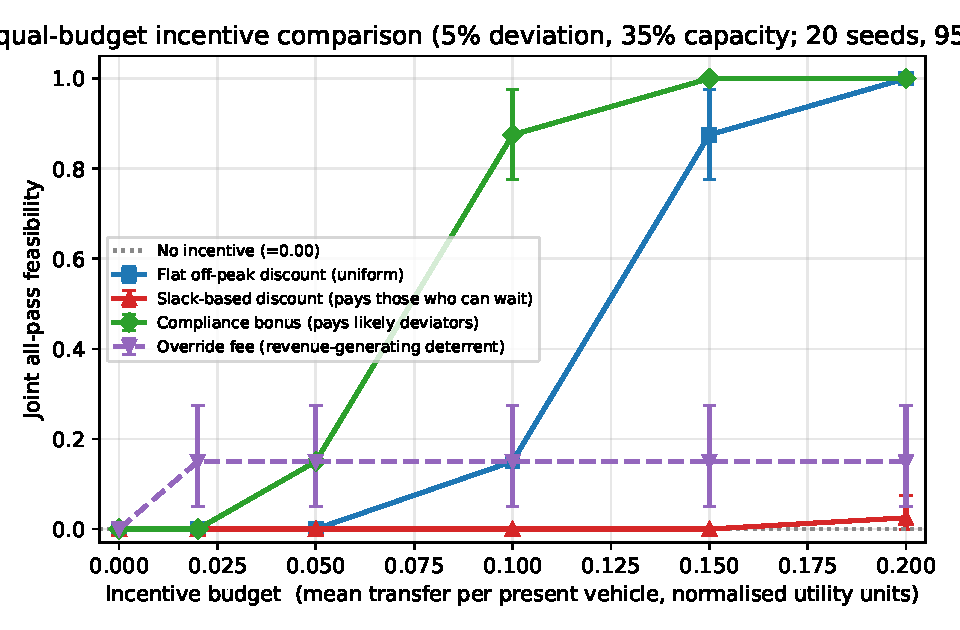
\includegraphics[width=0.72\textwidth]{figures/fig_incentive_comparison_20260716.pdf}
\caption{Equal-budget incentive comparison at the collapse point ($5\%$ deviation, $35\%$ charger capacity, both grid settings, 20 seeds, 95\% bootstrap CIs). All allocation rules spend the same average transfer per present vehicle (horizontal axis, normalised utility units). A compliance bonus targeted at the drivers most likely to override restores joint all-pass feasibility at a smaller budget than a uniform off-peak discount, whereas a slack-based discount that pays drivers who can already wait never restores it. A revenue-generating override fee (dashed) deters some deviation without spending budget but, at a strength matched to the flat discount, does not clear the compliance cliff and shifts cost onto drivers. Curves reflect the modelled compliance response, not measured field elasticities.}
\label{fig:incentive}
\end{figure}

This mechanism analysis shows the collapse is not a dead end: a transparent, bounded incentive paired with the grid signal moves the system from the uncoordinated equilibrium to a jointly acceptable point. We keep the claim bounded---the driver game is a \emph{calibrated behavioral model} (magnitude and slack anchored to data), not fitted to logged opt-out; the welfare weights are normative; and $\sigma$ is in normalised utility units, not a dollar tariff---so translating $\sigma^\star$ into a price schedule and fitting the compliance response to a trial remain the defined next steps.

% ---------------- figures ----------------
\begin{figure}[t]
\centering
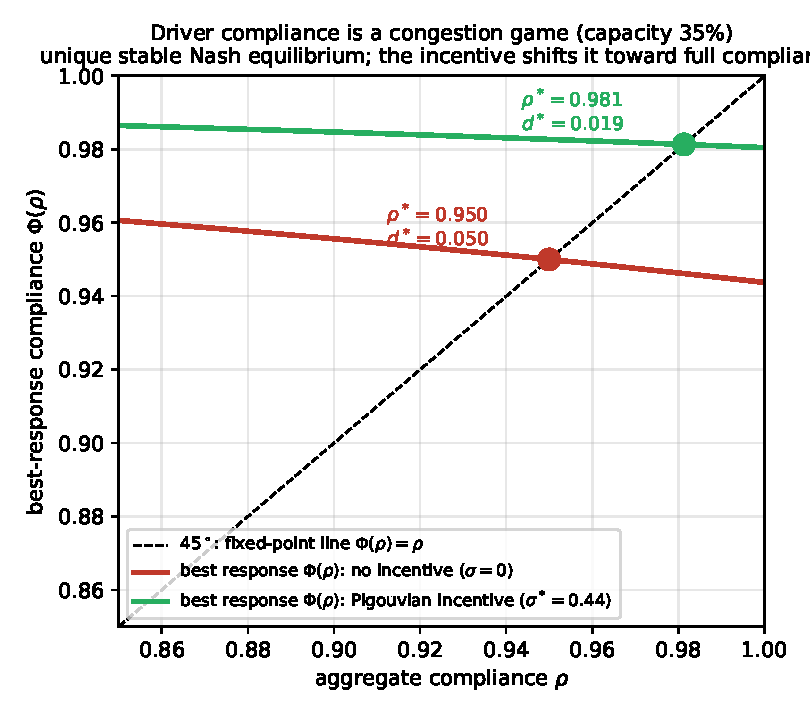
\includegraphics[width=0.62\textwidth]{figures/fig_eq_bestresponse.pdf}
\caption{Driver compliance as a congestion game (35\% capacity). The best-response
map $\Phi(\rho)$ crosses the $45^\circ$ line once, giving a unique stable Nash
equilibrium. With no incentive the equilibrium sits at compliance $\rho^\star=0.95$
(deviation $d^\star=0.05$), the ACN-anchored operating point at which same-episode
all-pass acceptability is zero; the Pigouvian-style incentive $\sigma^\star$ shifts the
best response up, moving the equilibrium toward full compliance.}
\label{fig:eqbr}
\end{figure}

\begin{figure}[t]
\centering
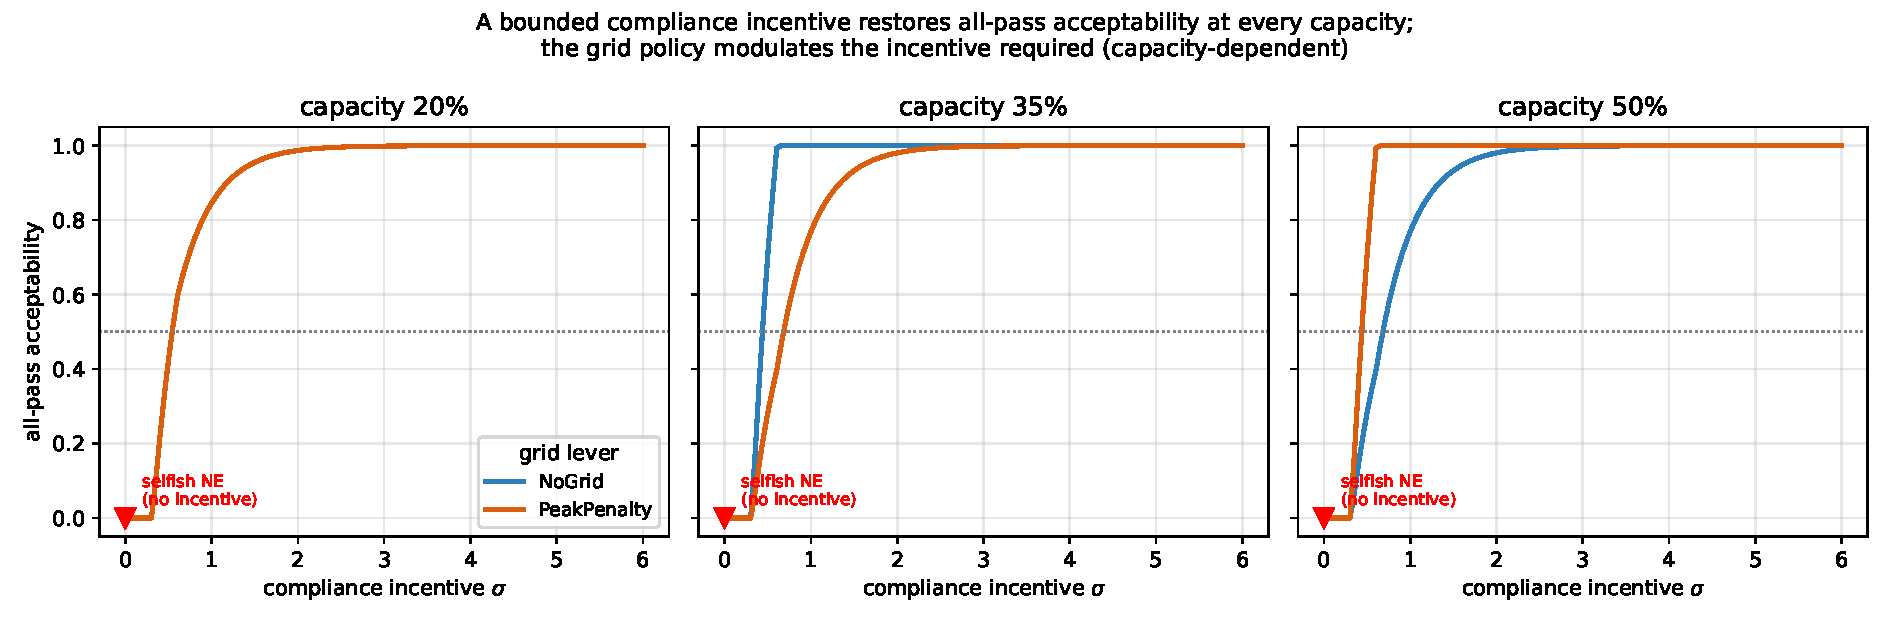
\includegraphics[width=0.74\textwidth]{figures/fig_eq_allpass_vs_incentive.pdf}
\caption{All-pass acceptability of the induced driver equilibrium as a function of the
compliance incentive $\sigma$, for the two grid policies at each capacity. The selfish
equilibrium ($\sigma=0$, red marker) is unacceptable; a bounded incentive restores
all-pass at every capacity. The grid policy modulates the incentive required, with a
capacity-dependent sign (GridPeakPenalty helps at $50\%$ capacity).}
\label{fig:eqap}
\end{figure}

\begin{figure}[t]
\centering
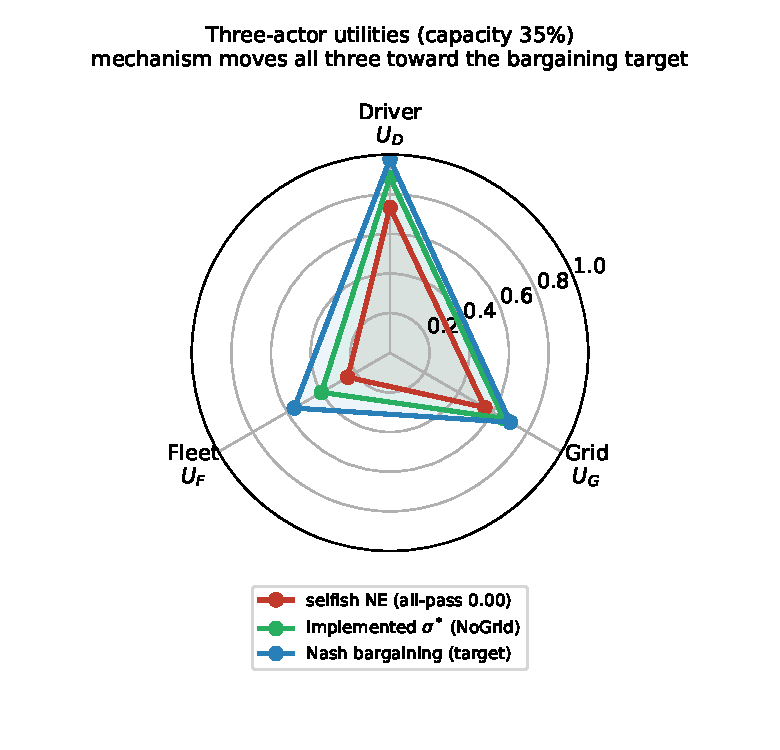
\includegraphics[width=0.6\textwidth]{figures/fig_eq_utility_triangle.pdf}
\caption{Driver, charging operator, and grid utilities (35\% capacity) at the selfish Nash
equilibrium, at the implemented incentive $\sigma^\star$, and at the cooperative Nash
bargaining solution. The charging operator is the worst-off actor under uncoordinated deviation; the
mechanism expands all three utilities toward the bargaining target.}
\label{fig:eqtri}
\end{figure}

\begin{figure}[t]
\centering
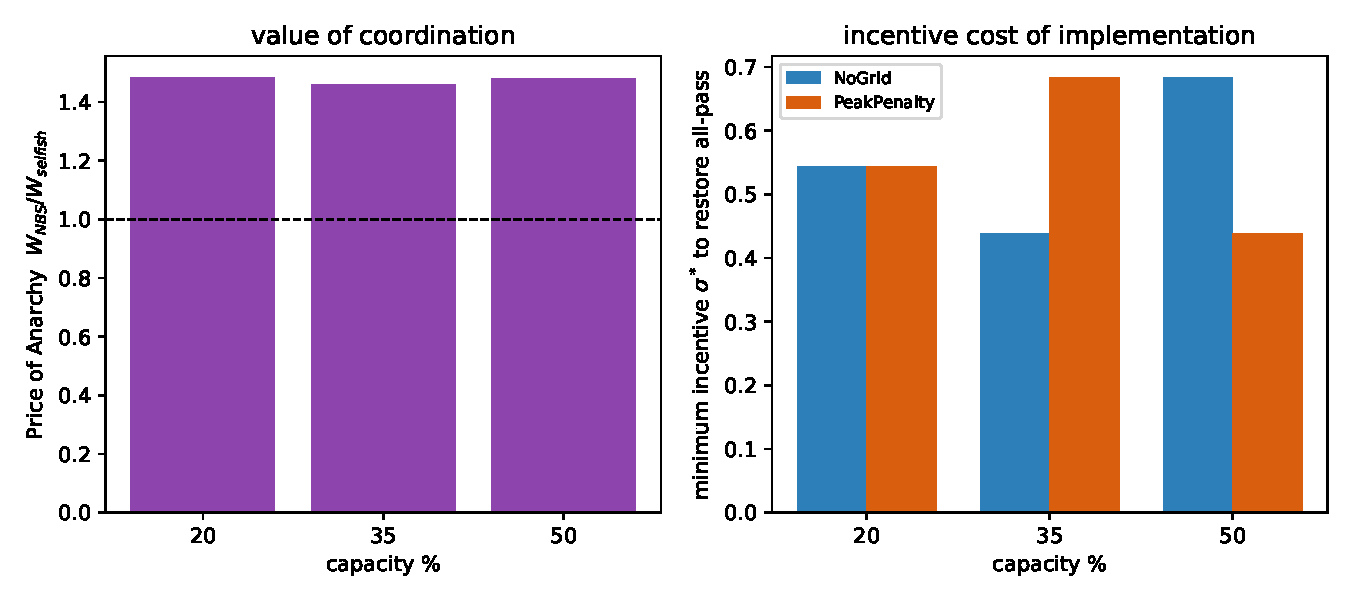
\includegraphics[width=0.72\textwidth]{figures/fig_eq_poa.pdf}
\caption{Left: price of anarchy $W_{\mathrm{NBS}}/W_{\mathrm{selfish}}$ by capacity
(coordination is worth roughly a $47\%$ welfare gain). Right: minimum incentive
$\sigma^\star$ that restores modelled all-pass, by capacity and grid policy.}
\label{fig:eqpoa}
\end{figure}

\section{Discussion}\label{sec:discussion}

The main practical implication is that EV charging control should be evaluated as a multi-actor energy-system problem. A policy may be active, feasible in a local simulator, and attractive under one metric while still being unacceptable to the actors required for deployment. The actor-gate framework makes that failure explicit. For a facility operator, the framework identifies whether service or operator service is the limiting concern. For grid planners, it distinguishes peak-ratio improvements from system acceptability. For researchers, it provides a claim discipline that prevents mechanism claims from outrunning trace evidence.

\paragraph{Applying the framework to a new site, city, or network.} The method is portable in five steps: (1)~\emph{specify participation constraints}---encode each actor's minimum requirement as a gate (driver service/reliability, operator queue/wait/cost, grid load-shape) with thresholds from local service-level agreements; (2)~\emph{calibrate demand} to local charging logs, as we do against ACN-Data; (3)~\emph{bracket compliance} from local opt-out/override rates, or sweep deviation as a stress test where such data are absent; (4)~\emph{compute and disaggregate feasibility} by capacity, binding gate, and behavior type (as in \figref{fig:eqdiag}); and (5)~\emph{choose the lever}---add capacity if infrastructure binds, or design a compliance incentive targeting the high-churn behavior if compliance binds. The output is a diagnosis, not a verdict. The \emph{portable} elements (reusable unchanged) are the conjunction logic, per-episode evaluation, request-pipeline audit, robustness protocol, and disaggregation diagnosis; the \emph{scenario-specific} choices are the gate set and thresholds, anchor policy, demand calibration, capacity, and compliance bracket. A threshold is justified for a new deployment not by matching our values but by being defensible against that deployment's own service-level commitments.

\paragraph{From the modeled incentive to deployable program design.} The model identifies \emph{what} the corrective lever must do and \emph{which} behavior it must target, but not its operational form: $\sigma^\star$ is in normalised utility units, and the diagnosis (Section~\ref{sec:diagnostic}) shows the binding cause is recommendation-override request churn---reserve- and price-driven overriding that breaks the driver's own critical-service gate---rather than benign inattention. This narrows the design space to instruments that raise compliance either by removing the \emph{reason} to override or by pricing the override, and lets each be matched to the diagnosed mechanism. Candidate operational embodiments, grounded in the managed-charging literature but not field-validated here, include: (i)~\emph{default managed charging} (opt-out rather than opt-in enrolment), the structural embodiment of a higher baseline compliance, since defaults are a strong participation lever and trials show active override is the failure mode \cite{dudek2021electricnation,alexeenko2023pilot}; (ii)~\emph{service guarantees}---a contractual trip-readiness guarantee in exchange for compliance---which directly removes the reserve- and deadline-anxiety motive for overriding that the diagnosis identifies \cite{schmalfuss2015,hardman2018}; (iii)~\emph{congestion-aware override pricing}, a small charge for \emph{discretionary} overrides, the most literal operational form of the Pigouvian internalisation that $\sigma$ models; (iv)~\emph{flexibility rewards or charging credits}, the carrot form of $\sigma$ at the few-dollars-per-session scale observed in pilots \cite{bailey2025fieldexp,wong2023incentives}, targeting the price-sensitive high-churn type; and (v)~\emph{eliciting departure time and minimum state of charge}, an information mechanism that lets the scheduler meet the genuine need and so removes the reason to override the recommendation, complementing the action-level levers. The mechanism-targeting counterfactual of Section~\ref{sec:results} (\figref{fig:instrument}) supports this design logic at the mechanism level: suppressing the recommendation-override override motive while holding the deviation rate fixed recovers same-episode feasibility from $0.00$ to $0.60$ at a $2.5\%$ rate, exactly the channel instruments~(ii)--(iii) act on. These remain design \emph{translations}, not validated policies, and we claim no dollar values, welfare-optimality, or measured effectiveness for them: instantiating any one requires the compliance-elasticity and monetary calibration we flag as future work (Section~\ref{sec:limitations}), and the counterfactual itself shows the instruments must be paired with raising compliance to clear higher deviation. The framework's role is to tell a deployer that this design effort---not further scheduling optimisation---is where the binding constraint lies, and to name the specific behavior it must target.

This same-episode screen is complementary to, not a replacement for, the multi-objective and Pareto analyses common in EV charging \cite{wang2024multiobj,das2020technoecon,woo2021}: a Pareto front characterises the trade-off surface aggregated over scenarios, but a point can be Pareto-efficient while violating one actor's requirement in a given episode. The added value is the explicit per-episode joint-satisfaction test, which localises which actor and metric bind first---shown concretely in Section~\ref{sec:results}, where a Pareto-efficient policy fails the conjunction (\figref{fig:pareto}) and a scenario-averaged read passes 11 of 14 gates while same-episode acceptability is $1.2\%$. The mechanism analysis (Section~\ref{sec:game}) then adds a constructive layer: the Nash bargaining solution identifies a fair point that clears the gates, and the Stackelberg incentive moves the equilibrium toward it. The contribution is thus the joint-feasibility lens \emph{together with} a calibrated mechanism analysis, not a new controller or a behavioral prediction.

Three interpretive cautions, detailed in the Limitations, carry the main caveats. The behavioral effect is request-event churn, not energy amplification, and the demanded-kWh ledger is an \emph{internal} consistency check (it balances to $10^{-4}$ kWh), not a field validation; grid-side PeakPenalty reduces peak ratios but does not rescue acceptability once driver and operator gates fail; and the IEEE-33 voltage screen is base-load-dominated, so only the relative line-loading, loss, and substation-peak deltas carry a policy signal.

\section{Limitations}\label{sec:limitations}

The study is simulation-only, and the behavioral-response layer is its main calibration gap. The charging-demand model is calibrated to and validated against real ACN-Data and cross-checked against ACN-Sim (Section~\ref{sec:extval}), and the grid physics uses a validated solver on a benchmark feeder. The behavioral severity levels are stress tests: their deviation \emph{magnitudes} are anchored to observed plan-deviation rates in the same ACN-Data (early disconnection, departure mismatch, and explicit input changes; Section~\ref{sec:design}), and the low-deviation level is low relative to those observed rates---though not directly comparable, because the severity parameter operates at the vehicle-timestep level rather than per session---but the within-level \emph{mechanism}---which vehicle-timesteps deviate and how the recommendation-override rule responds---is not fitted to observed session-level choices. In other words, the deviation magnitude is empirically anchored while its fine-grained temporal structure remains a model. Reading the magnitudes as deployment forecasts would still require fitting the response mechanism to a managed-charging dataset with logged opt-out/override decisions and validating against real feeder measurements.

The evidence base is moderate: each severity cell aggregates 240 episodes (twenty seeds, three capacities, two grid policies, two service operator policies), and reported intervals are bootstrap estimates over these episodes. The longer-horizon demanded-kWh trace and 28-day confirmation are targeted to the 35\% capacity service-oriented cases (five seeds, one capacity) rather than run exhaustively across capacities, so the $0\%$ 28-day figure is a single-capacity confirmation with higher per-estimate variance than the 20-seed weekly sweep, not an independent multi-capacity result; it should be read as consistent with, not a stronger generalization of, the weekly collapse. Larger seed counts and additional long-horizon capacity combinations would tighten the estimates.

The acceptability gates and their aggregation are normative. The thresholds are not universal constants, and the all-pass indicator is a strict conjunction of binary criteria that sharpens any degradation, so it should be read together with the graded fraction-of-criteria index rather than as a standalone cliff. Section~\ref{sec:robust} shows the qualitative conclusion is less sensitive across the tested threshold and aggregation choices, but selecting a single canonical rule and stakeholder-set cut-points for deployment decisions remains open.

The IEEE-33 feeder screen is representative rather than site-specific: it compares EV-off-relative deltas in substation peak, line loading, and losses but is not an interconnection study and does not validate feasibility for a real feeder.

ServiceGridWeighted is a fixed heuristic comparator, not an optimal controller; it reduces strawman-baseline risk and should not be read as state-of-the-art control.

The game-theoretic mechanism (Section~\ref{sec:game}) is a behavioral \emph{overlay}, not an agent-based strategic simulation: the simulator supplies the actor utilities and acceptability at each deviation level, while the compliance equilibrium is computed on a calibrated congestion game whose magnitude and slack are anchored to data but whose functional forms (linear externality, logistic cost heterogeneity) are assumed. We sweep parameters but not forms; the price of anarchy is a \emph{relative} welfare measure (min--max-normalised utilities); and $\sigma$ is in normalised utility units, not a monetary tariff (the charging operator-economics and monetary-mapping caveats are detailed in Section~\ref{sec:game} and the Supplement). The chief idealization is observability: the Stackelberg operator is assumed to know the compliance-response $\Phi$ and to observe $d^\star$. A live operator would instead infer compliance from charging-session logs (recommended versus delivered actions, opt-out/override rates)---the same decision-level data that fitting the mechanism requires and that we lack---separating genuine deviation from preference changes or faults, estimating $\Phi$ online, and absorbing measurement noise that propagates into $\sigma$. We therefore present the Stackelberg analysis as a characterization of the lever under known response, not an estimator deployable today; an online noise-robust estimator for $\Phi$, a deployable price-schedule translation of $\sigma^\star$, an endogenous agent-based strategic model, and fitting the compliance model to a trial with logged opt-out decisions are the defined next steps.

\section{Conclusions}\label{sec:conclusions}

This paper recasts the deployability of managed EV charging as multi-actor compliance \emph{feasibility}. Each actor gate is a participation constraint, an episode is feasible when the driver, charging operator, and grid constraints hold jointly, and the object of study is the feasible set and the probability the system lies inside it---not the optimum of a blended objective, because the actors' requirements are non-compensatory. We report the results as a two-part hypothesis, and the conclusions below are stated in those terms. The \emph{structural} claim (H1)---that within the modeled system joint feasibility has a compliance threshold that no scheduler or objective weighting we tested removes---we establish, and we treat it as having survived deliberate refutation attempts (a hindsight-optimal oracle and a full sweep of objective weightings, either of which could have broken it) rather than as merely robust. The \emph{empirical} claim (H2)---that real charging populations operate in that infeasible regime---our behavioral model frames but does not settle, because it is anchored to observed deviation magnitudes rather than fitted to field opt-out; closing that gap is the calibration study we flag as the key next step.

The evidence shows that service-oriented policies usually pass the conjunction under full compliance, though grid load-shape failures and capacity effects keep severity-0 acceptability below one, while low-deviation severity-1 behavior reduces same-episode all-pass acceptability to near zero under the current gates---to 1.2\% (95\% bootstrap interval $[0.0\%, 2.9\%]$) in the 20-seed weekly sweep, with a single-capacity 28-day check (35\% capacity, five seeds) consistent with this collapse rather than constituting an independent multi-capacity confirmation. Request-event pressure rises smoothly with severity, while the conjunction of driver, charging operator, and grid gates fails at severity 1. GridPeakPenalty can reduce selected peak ratios but does not rescue all-pass outcomes after driver and operator gates fail, and a hindsight-optimal oracle over the \emph{tested} scheduler menu reaches only $5\%$, so within that menu scheduler selection did not restore joint feasibility at the modeled deviation levels; we do not claim this over all possible charging controls. Applying the same framework to a data-grounded apartment (multi-unit-dwelling) scenario shows the collapse occurs in both tested charging ecologies but the binding actor is context-dependent: it shifts from driver service (workplace) to shared-charger capacity (apartment), while the apartment grid is buffered by overnight slack and de-stressed only as long as compliance holds (Section~\ref{sec:ecology}). These quantitative findings are established for US workplace and campus charging populations (the demand-validated ACN-Data sites), with the apartment case a scenario stress test rather than an empirically validated demand calibration; generalization to public fast-charge and to other non-US arrival patterns is left to future work.

The demanded-kWh audit classifies behavioral severity as request-event churn rather than true demanded-kWh amplification; event counts rise while simulator demanded kWh modestly falls.

In the calibrated congestion-game model the no-incentive equilibrium coincides with the acceptability collapse, and a bounded Pigouvian-style compliance incentive---set by the operator as a Stackelberg leader and paired with the grid signal---moves the equilibrium toward the cooperative Nash bargaining target and restores joint driver--operator--grid acceptability within the model. The relative price of anarchy is about 1.5, and these conclusions hold across the tested capacities and game parameters, so the diagnostic collapse comes with a constructive remedy---subject to calibrating the compliance mechanism to field data, which remains the key next step.

The contribution is a participation-feasibility account of managed-charging deployment: a feasible set defined by per-actor participation constraints; a concrete compliance threshold ($\sim$98.5\% recommendation adherence) below which feasibility collapses, robust to scheduler choice (least-laxity and earliest-deadline) and to the non-compliant preference form; and a congestion-game identification of a compliance incentive---not a better scheduler---as the operator's effective lever, with a relative price of anarchy near $1.5$. The demand layer is anchored in ACN-Data and ACN-Sim; the behavioral layer remains a model-assumed structure calibrated to deviation magnitudes, and fitting it to logged opt-out data is the natural next step. The central lesson is actionable: beyond a competent scheduler, the binding constraint for deploying managed charging is securing near-complete compliance---and compliance has \emph{two} equally-fragile axes, since feasibility collapses by roughly $5\%$ non-compliance whether drivers ignore the recommended action or misreport their needs to game a scarce shared resource (Section~\ref{sec:results}). Program operators, regulators, and tariff designers should therefore treat participation incentives---not further scheduling optimization---as the primary deployment lever. Because near-complete compliance cannot be assumed, it must be \emph{designed}: the modeled Pigouvian incentive points to concrete, literature-grounded instruments---default (opt-out) managed charging, service guarantees, flexibility rewards, congestion-aware override pricing, and eliciting departure time and minimum state of charge (Section~\ref{sec:discussion})---each targeting the specific recommendation-override overriding the diagnosis identifies. A mechanism-targeting counterfactual supports this at the mechanism level---suppressing the override motive at a fixed deviation rate recovers same-episode feasibility from $0.00$ to $0.60$ at $2.5\%$ deviation---while showing the instruments must be paired with raising compliance at higher deviation; they remain design translations requiring field calibration, not validated policies.

\section*{CRediT author statement}
Peijia Pok: Conceptualization, Methodology, Software, Formal analysis, Visualization, Writing -- original draft. Soomin Woo: Methodology, Validation, Writing -- review and editing. Hwasoo Yeo: Supervision, Project administration, Writing -- review and editing.

\section*{Declaration of competing interest}
The authors declare that they have no known competing financial interests or personal relationships that could have appeared to influence the work reported in this paper.

\section*{Data and code availability}
The analysis code, derived simulation outputs, and figure-generation scripts needed to reproduce the reported tables and figures are openly available, for review and after publication, at \url{https://github.com/peijiapok/multiactor}. The repository contains the game-theoretic equilibrium, Pareto-demonstration, scheduler-baseline (including the EDF anchor), and per-episode disaggregation analyses; the response-surface and severity-sweep result tables; and the figure-generation code. The charging-demand model is calibrated to the public ACN-Data dataset \cite{acndata2019}. The repository will be archived with a citable DOI (e.g., via Zenodo) at acceptance so that the reported tables and figures remain independently reproducible.

\begin{thebibliography}{99}
\bibitem{woo2021} S. Woo, S. Bae, S. J. Moura, Pareto optimality in cost and service quality for an Electric Vehicle charging facility, Applied Energy 290 (2021) 116779. \url{https://doi.org/10.1016/j.apenergy.2021.116779}.
\bibitem{ma2013} Z. Ma, D. S. Callaway, I. A. Hiskens, Decentralized charging control of large populations of plug-in electric vehicles, IEEE Transactions on Control Systems Technology 21(1) (2013) 67--78. \url{https://doi.org/10.1109/TCST.2011.2174059}.
\bibitem{gan2013} L. Gan, U. Topcu, S. H. Low, Optimal decentralized protocol for electric vehicle charging, IEEE Transactions on Power Systems 28(2) (2013) 940--951. \url{https://doi.org/10.1109/TPWRS.2012.2210288}.
\bibitem{sortomme2011} E. Sortomme, M. A. El-Sharkawi, Optimal charging strategies for unidirectional vehicle-to-grid, IEEE Transactions on Smart Grid 2(1) (2011) 131--138. \url{https://doi.org/10.1109/TSG.2010.2090910}.
\bibitem{lee2021adaptive} Z. J. Lee, G. S. Lee, T. Lee, C. Jin, R. Lee, Z. Low, D. Chang, C. Ortega, S. H. Low, Adaptive charging networks: A framework for smart electric vehicle charging, IEEE Transactions on Smart Grid 12(5) (2021) 4339--4350. \url{https://doi.org/10.1109/TSG.2021.3074437}.
\bibitem{liu1973scheduling} C. L. Liu, J. W. Layland, Scheduling algorithms for multiprogramming in a hard-real-time environment, Journal of the ACM 20(1) (1973) 46--61. \url{https://doi.org/10.1145/321738.321743}.
\bibitem{dertouzos1989llf} M. L. Dertouzos, A. K. Mok, Multiprocessor on-line scheduling of hard-real-time tasks, IEEE Transactions on Software Engineering 15(12) (1989) 1497--1506. \url{https://doi.org/10.1109/32.58762}.
\bibitem{lee2019acnsim} Z. J. Lee, S. Sharma, D. Johansson, S. H. Low, ACN-Sim: An open-source simulator for data-driven electric vehicle charging research, IEEE SmartGridComm (2019). \url{https://doi.org/10.1109/SmartGridComm.2019.8909765}.
\bibitem{acndata2019} Z. J. Lee, T. Li, S. H. Low, ACN-Data: Analysis and applications of an open EV charging dataset, in: Proceedings of the Tenth ACM International Conference on Future Energy Systems (e-Energy '19) (2019) 139--149. \url{https://doi.org/10.1145/3307772.3328313}.
\bibitem{will2016} C. Will, A. Schuller, Understanding user acceptance factors of electric vehicle smart charging, Transportation Research Part C 71 (2016) 198--214. \url{https://doi.org/10.1016/j.trc.2016.07.006}.
\bibitem{bailey2015} J. Bailey, J. Axsen, Anticipating PEV buyers' acceptance of utility controlled charging, Transportation Research Part A 82 (2015) 29--46. \url{https://doi.org/10.1016/j.tra.2015.09.004}.
\bibitem{schmalfuss2015} N. Schmalfuss, K. Muhl, J. F. Krems, User responses to a smart charging system in Germany: Battery electric vehicle driver motivation, attitudes and acceptance, Energy Research \& Social Science 9 (2015) 60--71. \url{https://doi.org/10.1016/j.erss.2015.08.019}.
\bibitem{delmonte2020} E. Delmonte, N. Kinnear, B. Jenkins, S. Skippon, What do consumers think of smart charging? Perceptions among actual and potential plug-in electric vehicle adopters in the United Kingdom, Energy Research \& Social Science 60 (2020) 101318. \url{https://doi.org/10.1016/j.erss.2019.101318}.
\bibitem{tarroja2021} B. Tarroja, E. Hittinger, The value of consumer acceptance of controlled electric vehicle charging in a decarbonizing grid: The case of California, Energy 229 (2021) 120691. \url{https://doi.org/10.1016/j.energy.2021.120691}.
\bibitem{danner2021} D. Danner, H. de Meer, Quality of service and fairness for electric vehicle charging as a service, Energy Informatics 4(Suppl 3) (2021) 16. \url{https://doi.org/10.1186/s42162-021-00175-3}.
\bibitem{clement2010} K. Clement-Nyns, E. Haesen, J. Driesen, The impact of charging plug-in hybrid electric vehicles on a residential distribution grid, IEEE Transactions on Power Systems 25(1) (2010) 371--380. \url{https://doi.org/10.1109/TPWRS.2009.2036481}.
\bibitem{elnozahy2014} M. S. ElNozahy, M. M. A. Salama, A comprehensive study of the impacts of PHEVs on residential distribution networks, IEEE Transactions on Sustainable Energy 5(1) (2014) 332--342. \url{https://doi.org/10.1109/TSTE.2013.2284573}.
\bibitem{baran1989} M. E. Baran, F. F. Wu, Network reconfiguration in distribution systems for loss reduction and load balancing, IEEE Transactions on Power Delivery 4(2) (1989) 1401--1407. \url{https://doi.org/10.1109/61.25627}.
\bibitem{thurner2018} L. Thurner, A. Scheidler, F. Schafer, J.-H. Menke, J. Dollichon, F. Meier, S. Meinecke, M. Braun, Pandapower--an open-source Python tool for convenient modeling, analysis, and optimization of electric power systems, IEEE Transactions on Power Systems 33(6) (2018) 6510--6521. \url{https://doi.org/10.1109/TPWRS.2018.2829021}.
\bibitem{pandapowerdoc} pandapower development team, pandapower documentation, official documentation (accessed 10 June 2026). \url{https://pandapower.readthedocs.io/}.
\bibitem{richardson2013} D. B. Richardson, Electric vehicles and the electric grid: A review of modeling approaches, impacts, and renewable energy integration, Renewable and Sustainable Energy Reviews 19 (2013) 247--254. \url{https://doi.org/10.1016/j.rser.2012.11.042}.
\bibitem{green2011} R. C. Green, L. Wang, M. Alam, The impact of plug-in hybrid electric vehicles on distribution networks: A review and outlook, Renewable and Sustainable Energy Reviews 15(1) (2011) 544--553. \url{https://doi.org/10.1016/j.rser.2010.08.015}.
\bibitem{muratori2018} M. Muratori, Impact of uncoordinated plug-in electric vehicle charging on residential power demand, Nature Energy 3(3) (2018) 193--201. \url{https://doi.org/10.1038/s41560-017-0074-z}.
\bibitem{dubey2015} A. Dubey, S. Santoso, Electric vehicle charging on residential distribution systems: Impacts and mitigations, IEEE Access 3 (2015) 1871--1893. \url{https://doi.org/10.1109/ACCESS.2015.2476996}.
\bibitem{pieltain2011} L. Pieltain Fernandez, T. G. San Roman, R. Cossent, C. M. Domingo, P. Frias, Assessment of the impact of plug-in electric vehicles on distribution networks, IEEE Transactions on Power Systems 26(1) (2011) 206--213. \url{https://doi.org/10.1109/TPWRS.2010.2049133}.
\bibitem{lopes2011} J. A. P. Lopes, F. J. Soares, P. M. R. Almeida, Integration of electric vehicles in the electric power system, Proceedings of the IEEE 99(1) (2011) 168--183. \url{https://doi.org/10.1109/JPROC.2010.2066250}.
\bibitem{rotering2011} N. Rotering, M. Ilic, Optimal charge control of plug-in hybrid electric vehicles in deregulated electricity markets, IEEE Transactions on Power Systems 26(3) (2011) 1021--1029. \url{https://doi.org/10.1109/TPWRS.2010.2086083}.
\bibitem{nimalsiri2020} N. I. Nimalsiri, C. P. Mediwaththe, E. L. Ratnam, M. Shaw, D. B. Smith, S. K. Halgamuge, A survey of algorithms for distributed charging control of electric vehicles in smart grid, IEEE Transactions on Intelligent Transportation Systems 21(11) (2020) 4497--4515. \url{https://doi.org/10.1109/TITS.2019.2943620}.
\bibitem{powell2022} S. Powell, G. V. Cezar, L. Min, I. M. L. Azevedo, R. Rajagopal, Charging infrastructure access and operation to reduce the grid impacts of deep electric vehicle adoption, Nature Energy 7(10) (2022) 932--945. \url{https://doi.org/10.1038/s41560-022-01105-7}.
\bibitem{sovacool2018} B. K. Sovacool, L. Noel, J. Axsen, W. Kempton, The neglected social dimensions to a vehicle-to-grid (V2G) transition: A critical and systematic review, Environmental Research Letters 13(1) (2018) 013001. \url{https://doi.org/10.1088/1748-9326/aa9c6d}.
\bibitem{hardman2018} S. Hardman, A. Jenn, G. Tal, J. Axsen, G. Beard, N. Daina, E. Figenbaum, N. Jakobsson, et al., A review of consumer preferences of and interactions with electric vehicle charging infrastructure, Transportation Research Part D: Transport and Environment 62 (2018) 508--523. \url{https://doi.org/10.1016/j.trd.2018.04.002}.
\bibitem{funke2019} S. A. Funke, F. Sprei, T. Gnann, P. Plotz, How much charging infrastructure do electric vehicles need? A review of the evidence and international comparison, Transportation Research Part D: Transport and Environment 77 (2019) 224--242. \url{https://doi.org/10.1016/j.trd.2019.10.024}.
\bibitem{quiros2018} J. Quiros-Tortos, A. Navarro-Espinosa, L. F. Ochoa, T. Butler, Statistical representation of EV charging: Real data analysis and applications, 2018 Power Systems Computation Conference (PSCC) (2018) 1--7. \url{https://doi.org/10.23919/PSCC.2018.8442988}.
\bibitem{pournaras2019} E. Pournaras, S. Jung, S. Yadhunathan, H. Zhang, X. Fang, Socio-technical smart grid optimization via decentralized charge control of electric vehicles, Applied Soft Computing 82 (2019) 105573. \url{https://doi.org/10.1016/j.asoc.2019.105573}.
\bibitem{sadeghian2022} O. Sadeghian, A. Oshnoei, B. Mohammadi-ivatloo, V. Vahidinasab, A. Anvari-Moghaddam, A comprehensive review on electric vehicles smart charging: Solutions, strategies, technologies, and challenges, Journal of Energy Storage 54 (2022) 105241. \url{https://doi.org/10.1016/j.est.2022.105241}.
\bibitem{shaukat2018} N. Shaukat, B. Khan, S. M. Ali, C. A. Mehmood, J. Khan, U. Farid, M. Majid, S. M. Anwar, et al., A survey on electric vehicle transportation within smart grid system, Renewable and Sustainable Energy Reviews 81 (2018) 1329--1349. \url{https://doi.org/10.1016/j.rser.2017.05.092}.
\bibitem{richardson2012local} P. Richardson, D. Flynn, A. Keane, Local versus centralized charging strategies for electric vehicles in low voltage distribution systems, IEEE Transactions on Smart Grid 3(2) (2012) 1020--1028. \url{https://doi.org/10.1109/TSG.2012.2185523}.
\bibitem{alexeenko2023pilot} P. Alexeenko, E. Bitar, Achieving reliable coordination of residential plug-in electric vehicle charging: A pilot study, Transportation Research Part D: Transport and Environment 118 (2023) 103658. \url{https://doi.org/10.1016/j.trd.2023.103658}.
\bibitem{dudek2021electricnation} E. Dudek, The flexibility of domestic electric vehicle charging: The Electric Nation project, IEEE Power and Energy Magazine 19(4) (2021) 16--27. \url{https://doi.org/10.1109/MPE.2021.3072714}.
\bibitem{bailey2025fieldexp} M. R. Bailey, D. P. Brown, B. Shaffer, F. A. Wolak, Show me the money! A field experiment on electric vehicle charge timing, American Economic Journal: Economic Policy 17(2) (2025) 259--284. \url{https://doi.org/10.1257/pol.20230653}.
\bibitem{wong2023incentives} S. D. Wong, S. A. Shaheen, E. Martin, R. Uyeki, Do incentives make a difference? Understanding smart charging program adoption for electric vehicles, Transportation Research Part C: Emerging Technologies 151 (2023) 104123. \url{https://doi.org/10.1016/j.trc.2023.104123}.
\bibitem{tan2023fair} M. Tan, Y. Ren, R. Pan, L. Wang, J. Chen, Fair and efficient electric vehicle charging scheduling optimization considering the maximum individual waiting time and operating cost, IEEE Transactions on Vehicular Technology 72(8) (2023) 9808--9820. \url{https://doi.org/10.1109/TVT.2023.3257547}.
\bibitem{tsaousoglou2023fair} G. Tsaousoglou, J. S. Giraldo, P. Pinson, N. G. Paterakis, Fair and scalable electric vehicle charging under electrical grid constraints, IEEE Transactions on Intelligent Transportation Systems 24(12) (2023) 15169--15177. \url{https://doi.org/10.1109/TITS.2023.3311509}.
\bibitem{theodoropoulos2022proportional} T. Theodoropoulos, P. Pantazopoulos, E. Karfopoulos, P. Lytrivis, G. Karaseitanidis, A. Amditis, Proportionally fair and scalable EV charging under distribution line voltage constraints, Electric Power Systems Research 208 (2022) 107797. \url{https://doi.org/10.1016/j.epsr.2022.107797}.
\bibitem{wang2024multiobj} Y. Wang, H. Wang, R. Razzaghi, M. Jalili, A. Liebman, Multi-objective coordinated EV charging strategy in distribution networks using an improved augmented epsilon-constrained method, Applied Energy 369 (2024) 123547. \url{https://doi.org/10.1016/j.apenergy.2024.123547}.
\bibitem{das2020technoecon} R. Das, Y. Wang, G. Putrus, R. Kotter, M. Marzband, B. Herteleer, J. Warmerdam, Multi-objective techno-economic-environmental optimisation of electric vehicle for energy services, Applied Energy 257 (2020) 113965. \url{https://doi.org/10.1016/j.apenergy.2019.113965}.
\bibitem{liu2019decentralized} M. Liu, P. K. Phanivong, Y. Shi, D. S. Callaway, Decentralized charging control of electric vehicles in residential distribution networks, IEEE Transactions on Control Systems Technology 27(1) (2019) 266--281. \url{https://doi.org/10.1109/TCST.2017.2771307}.
\bibitem{liu2024busdepot} X. Liu, S. Yeh, P. Pl\"otz, W. Ma, F. Li, X. Ma, Electric bus charging scheduling problem considering charging infrastructure integrated with solar photovoltaic and energy storage systems, Transportation Research Part E: Logistics and Transportation Review 187 (2024) 103572. \url{https://doi.org/10.1016/j.tre.2024.103572}.
\bibitem{passow2025fleet} F. H. Passow, R. Rajagopal, Charging electrified commercial vehicle fleets with reduced grid capacity using low-capital-cost depot management strategies, Applied Energy 401 (2025) 126563. \url{https://doi.org/10.1016/j.apenergy.2025.126563}.
\bibitem{wang2009mcda} J.-J. Wang, Y.-Y. Jing, C.-F. Zhang, J.-H. Zhao, Review on multi-criteria decision analysis aid in sustainable energy decision-making, Renewable and Sustainable Energy Reviews 13(9) (2009) 2263--2278. \url{https://doi.org/10.1016/j.rser.2009.06.021}.

\bibitem{mcfadden1974} D. McFadden, Conditional logit analysis of qualitative choice behavior, in: P. Zarembka (Ed.), Frontiers in Econometrics, Academic Press, New York, 1974, pp. 105--142.

\bibitem{daina2017} N. Daina, A. Sivakumar, J. W. Polak, Electric vehicle charging choices: Modelling and implications for smart charging services, Transportation Research Part C: Emerging Technologies 81 (2017) 36--56. \url{https://doi.org/10.1016/j.trc.2017.05.006}.
\bibitem{wustenhagen2007acceptance} R. W\"ustenhagen, M. Wolsink, M. J. B\"urer, Social acceptance of renewable energy innovation: An introduction to the concept, Energy Policy 35(5) (2007) 2683--2691. \url{https://doi.org/10.1016/j.enpol.2006.12.001}.
\bibitem{marxen2023flexibility} H. Marxen, M. Ansarin, R. Chemudupaty, G. Fridgen, Empirical evaluation of behavioral interventions to enhance flexibility provision in smart charging, Transportation Research Part D: Transport and Environment 123 (2023) 103897. \url{https://doi.org/10.1016/j.trd.2023.103897}.

\end{thebibliography}

\clearpage
\section*{Supplementary material}\label{sec:supp}

\renewcommand{\thefigure}{S\arabic{figure}}
\setcounter{figure}{0}
\renewcommand{\thetable}{S\arabic{table}}
\setcounter{table}{0}

\subsection*{Supplementary figures}

\begin{figure}[H]
\centering
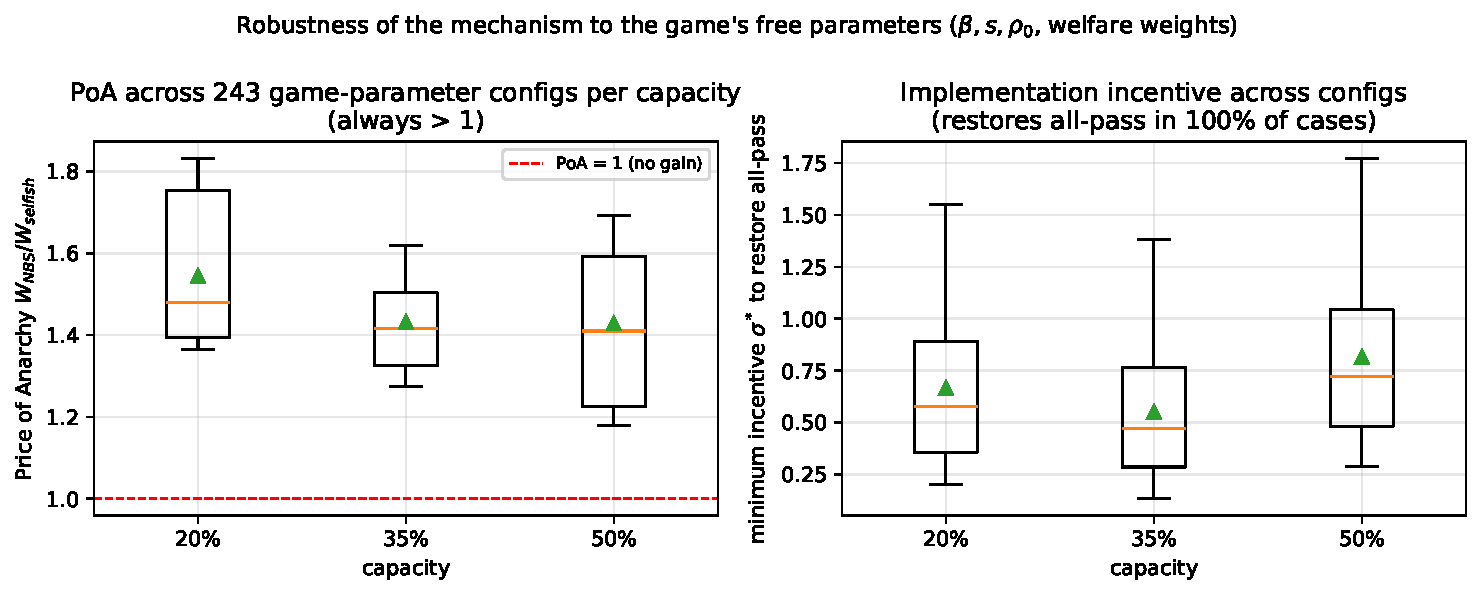
\includegraphics[width=0.95\textwidth]{figures/fig_eq_sensitivity.pdf}
\caption{Robustness of the game-theoretic mechanism (Section~\ref{sec:game}) to the game's free parameters. Across $243$ combinations of externality strength $\beta\in\{1,2,4\}$, cost-heterogeneity scale $s\in\{0.25,0.4,0.6\}$, compliance anchor $\rho_0\in\{0.90,0.95,0.97\}$, and three welfare-weight sets per capacity, the price of anarchy is always above one (left) and the minimum incentive $\sigma^\star$ restores modelled all-pass in every tested configuration (right). The selfish equilibrium is unique with all-pass $=0.000$ throughout.}
\label{fig:eqsens}
\end{figure}

\begin{figure}[H]
\centering
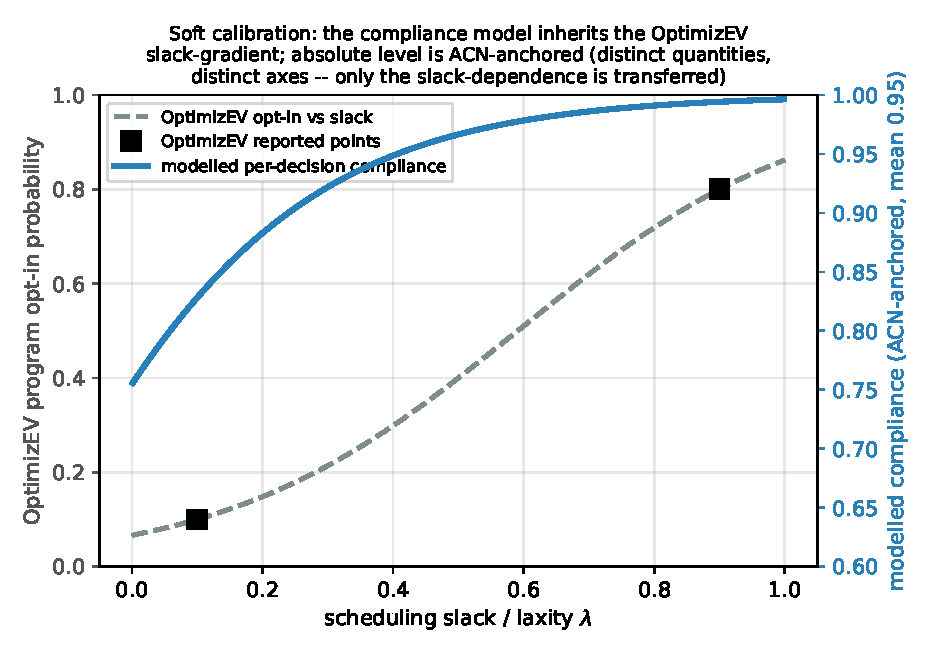
\includegraphics[width=0.62\textwidth]{figures/fig_eq_optimizev_calibration.pdf}
\caption{Soft calibration of the driver compliance model (Section~\ref{sec:game}) to the OptimizEV managed-charging pilot \cite{alexeenko2023pilot}. The model's slack-gradient is taken from the OptimizEV opt-in-versus-slack curve (gray dashed, left axis; black squares are the reported low- and high-slack opt-in values), while the absolute compliance level is anchored to the ACN deviation magnitude (blue, right axis, mean $0.95$). Program opt-in and per-decision compliance are different quantities shown on different axes; only the monotone slack-dependence is transferred.}
\label{fig:eqcalib}
\end{figure}

\paragraph{Operator economics: why service, not energy cost.} A charging operator ultimately cares about money, so we tested a profit-weighted operator objective (delivered-energy revenue minus normalised energy and demand-charge cost) in place of the service utility $U_O$ of Section~\ref{sec:game}. It is \emph{less} informative here, for a revealing reason: as deviation rises the simulator's delivered energy and its cost fall almost in lockstep, and the demand charge is insensitive to deviation, so a pure energy-cost-profit objective is near-neutral to deviation---even mildly rewarding it---rather than harmed (Fig.~\ref{fig:eqfleet}). Under that objective the relative price of anarchy weakens from $1.46$--$1.48$ to $1.05$--$1.33$ across capacities, because the cost saving from undelivered energy offsets the lost service revenue. This is precisely why we model the charging operator on the service/availability channel: that is where deviation actually threatens operator revenue (missed trips), whereas the energy and demand-charge cost belongs in the operator gate. Two simulator features drive the offset---synthetic-scale cost units and a demand charge that does not respond to behavioral churn---and both understate real operator cost exposure: in deployment, uncoordinated charging typically \emph{raises} demand charges, a operator's largest cost lever, which would strengthen rather than weaken the charging operator's exposure to deviation. We therefore report the charging operator result as a service/revenue finding and treat the profit-objective sensitivity as a check that the conclusion is not an artifact of excluding costs.

\begin{figure}[H]
\centering
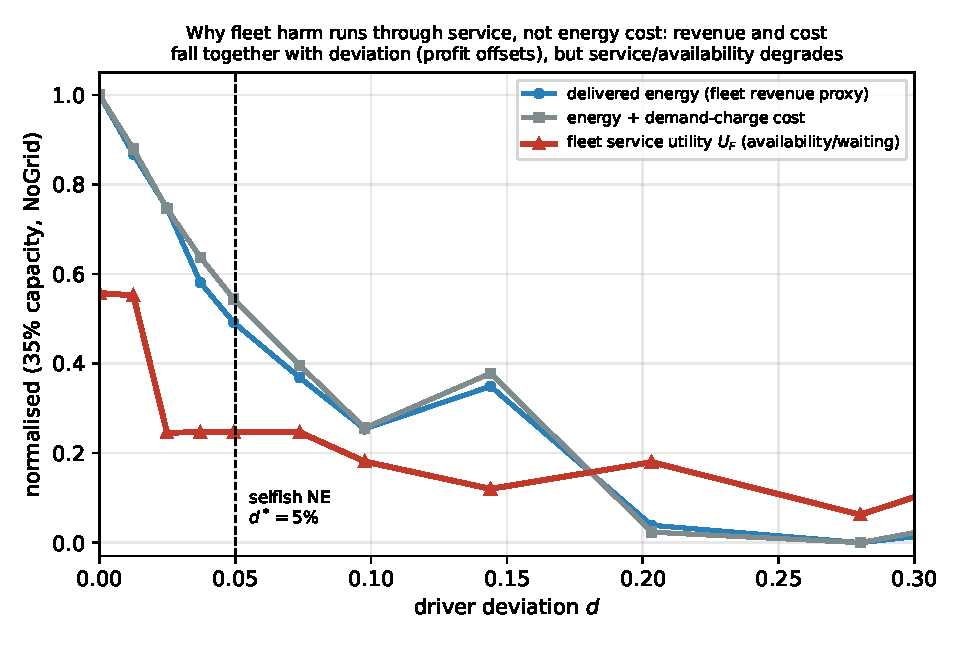
\includegraphics[width=0.66\textwidth]{figures/fig_eq_fleet_profit.pdf}
\caption{Operator-economics robustness (Section~\ref{sec:game}; $35\%$ capacity, NoGridAdjustment). As driver deviation rises, the charging operator revenue proxy (delivered energy) and the operator cost (energy plus demand charge) fall almost in lockstep, so a profit objective offsets to near-neutral; the demand charge itself is insensitive to deviation. The operator service/availability utility $U_O$, by contrast, degrades. This is why the charging operator's economic exposure to deviation is modelled through the service/revenue channel (missed trips), with energy and demand-charge cost handled in the operator gate; a profit-weighted objective weakens the relative price of anarchy to $1.05$--$1.33$ through this cost-offset.}
\label{fig:eqfleet}
\end{figure}

\begin{figure}[H]
\centering
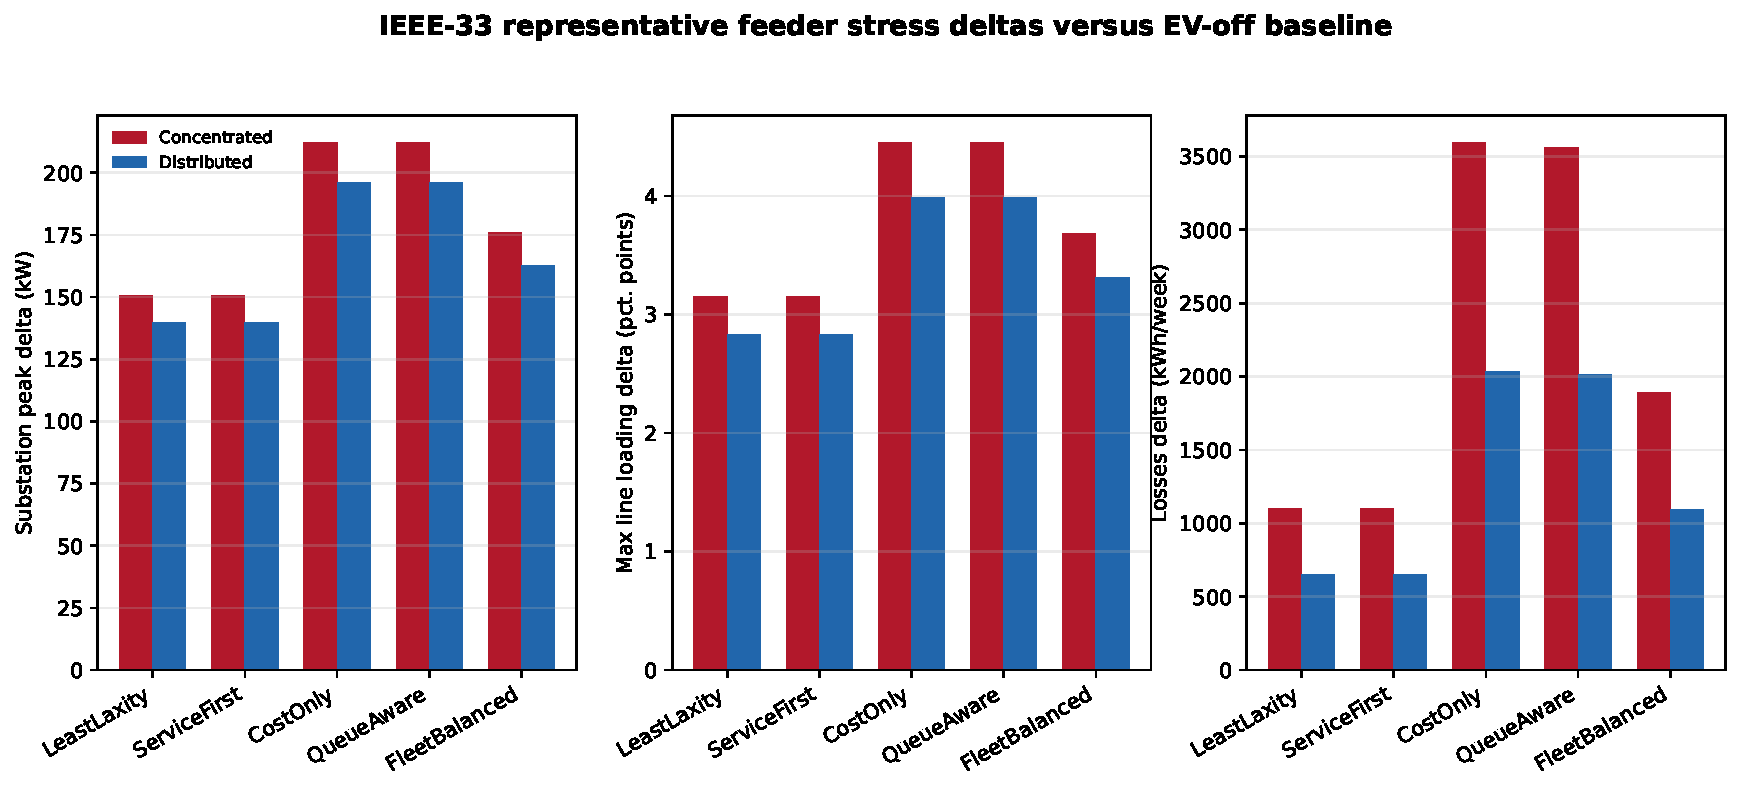
\includegraphics[width=0.9\textwidth]{figures/fig6_ieee33_feeder_deltas.pdf}
\caption{IEEE-33 representative feeder stress-screen deltas (Section~\ref{sec:results}). EV charging policies produce EV-off-relative feeder stress increments in substation peak, line loading, and losses; voltage-violation deltas are exactly zero in all 900 cases. The screen is an external grid-stress lens, not site-specific feeder validation.}
\label{fig:ieee33}
\end{figure}

\begin{figure}[H]
\centering
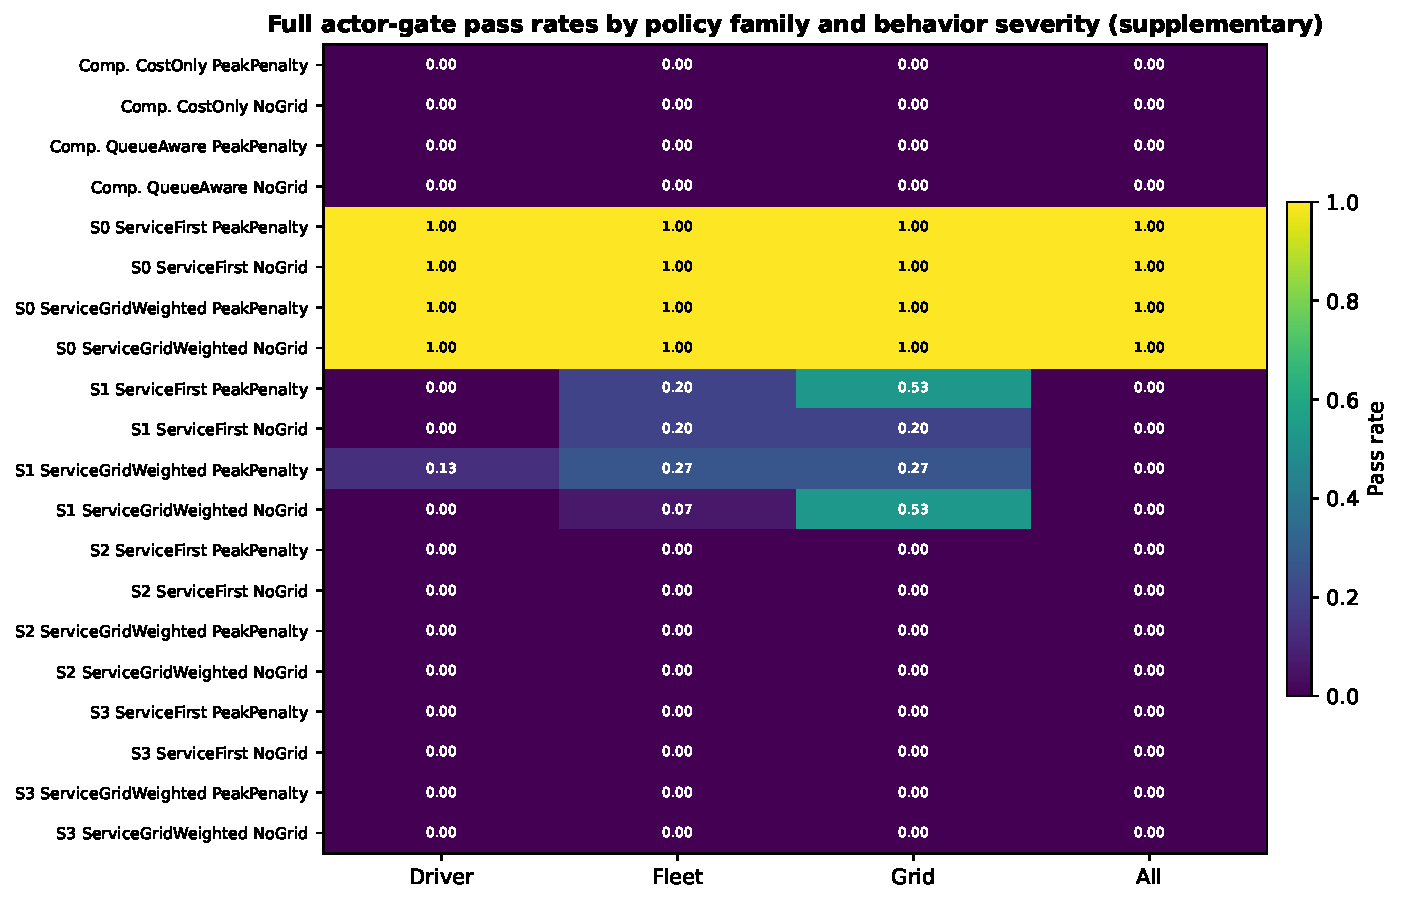
\includegraphics[width=0.9\textwidth]{figures/supp_full_actor_gate_matrix.pdf}
\caption{Full actor-gate matrix: pass rates for every policy (including the diagnostic CostOnly and QueueAware comparators) by behavior severity and grid policy. The condensed main-text \figref{fig:matrix} summarizes the service-oriented family from this matrix.}
\label{fig:suppmatrix}
\end{figure}

\begin{figure}[H]
\centering
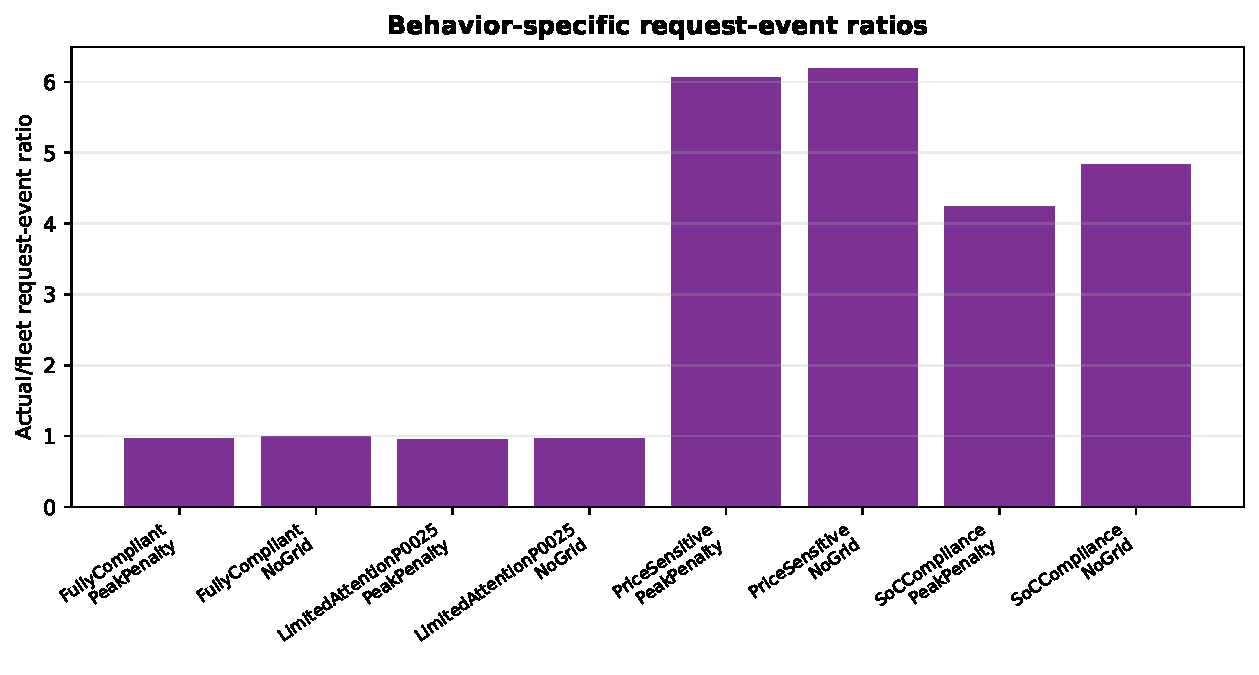
\includegraphics[width=0.9\textwidth]{figures/supp_request_id_conservation_audit.pdf}
\caption{Behavior-specific request-event ratios (actual driver-layer events relative to operator recommendations) by behavior model and grid policy; price-sensitive and SoC-compliance behaviors generate the most request-event churn. In the accompanying request-ID conservation audit the maximum count residual is exactly zero in every case, confirming that request identifiers are conserved across the driver, charging operator, and grid layers.}
\label{fig:suppcons}
\end{figure}

\begin{figure}[H]
\centering
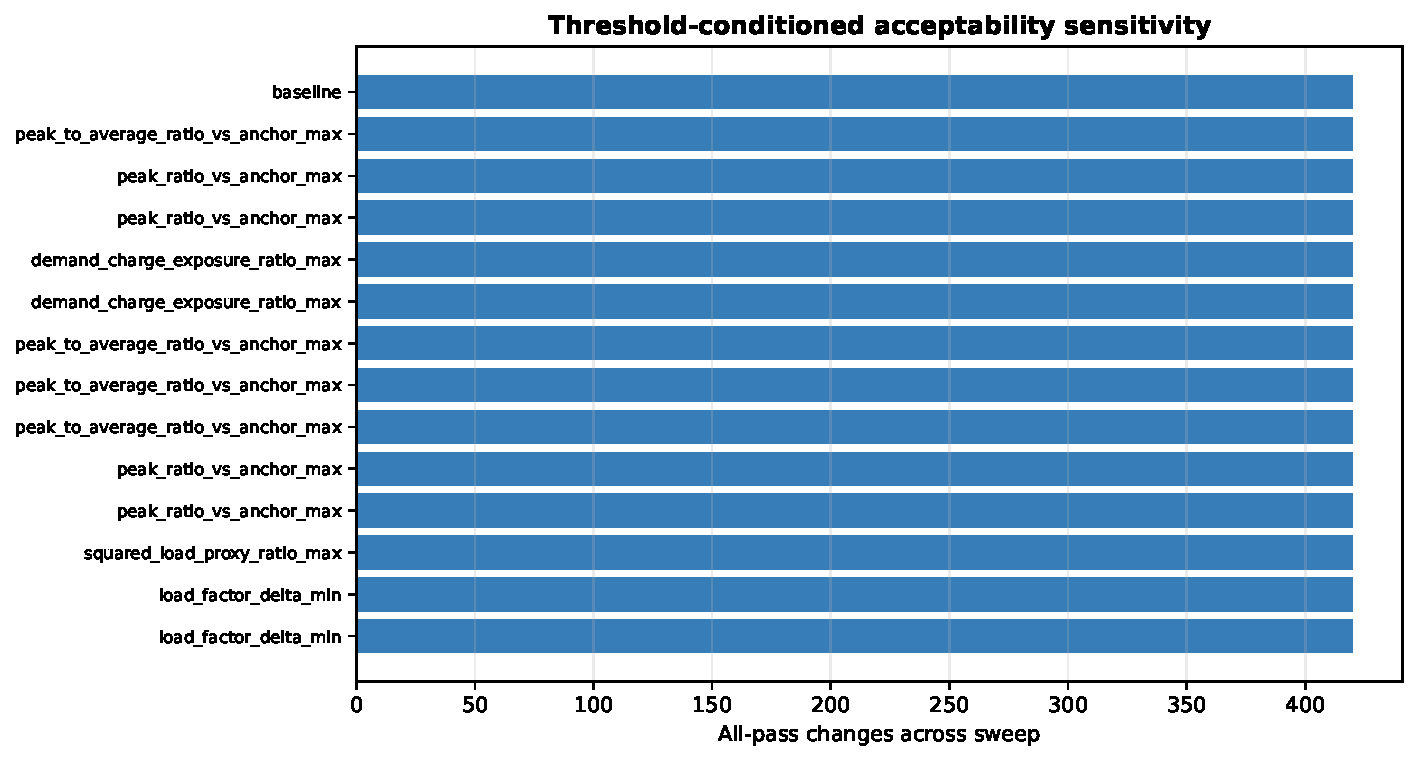
\includegraphics[width=0.9\textwidth]{figures/supp_threshold_sensitivity.pdf}
\caption{Threshold sensitivity: all-pass counts as the driver, charging operator, and grid gate thresholds are swept. Tightening the delivered-ratio gate reduces severity-0 all-pass rows, while the severity-1 collapse is preserved across the tested settings (see Section~\ref{sec:robust}).}
\label{fig:suppthresh}
\end{figure}

\begin{figure}[H]
\centering
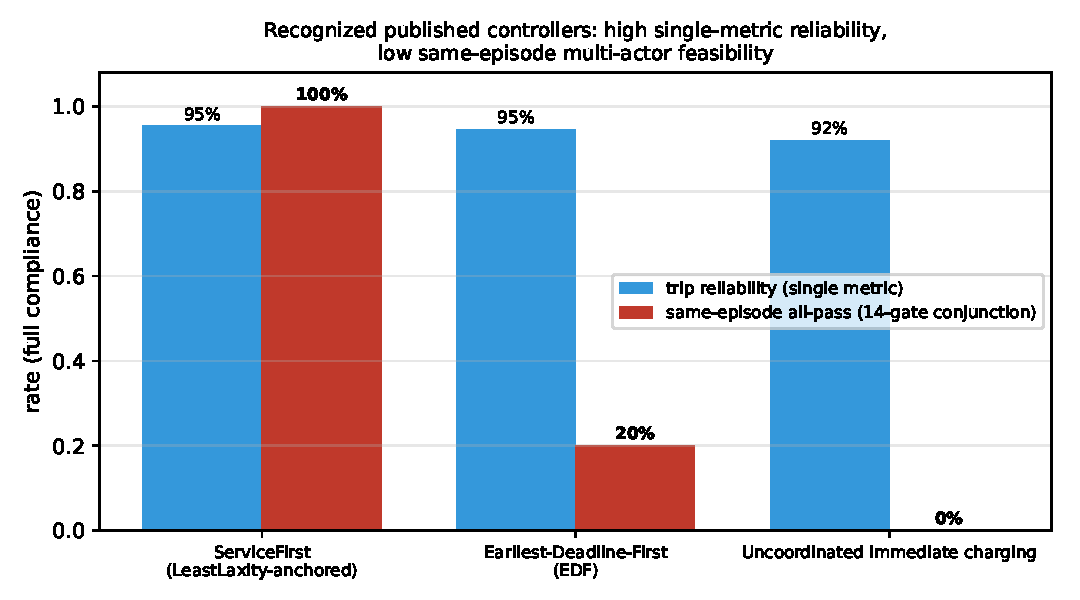
\includegraphics[width=0.7\textwidth]{figures/fig_published_controllers.pdf}
\caption{Recognized published controllers at full compliance (Section~\ref{sec:published}): high single-metric trip reliability ($91.9$--$95.9\%$, blue) but low same-episode 14-gate feasibility (red). EDF \cite{liu1973scheduling} passes the operator and grid gates entirely yet clears the conjunction in only $20\%$ of episodes (relative critical-service driver gate); uncoordinated immediate charging \cite{clement2010,ma2013} scores $0\%$ through congestion and load shape. The framework discriminates among established controllers rather than rejecting them uniformly.}
\label{fig:published}
\end{figure}

\begin{figure}[H]
\centering
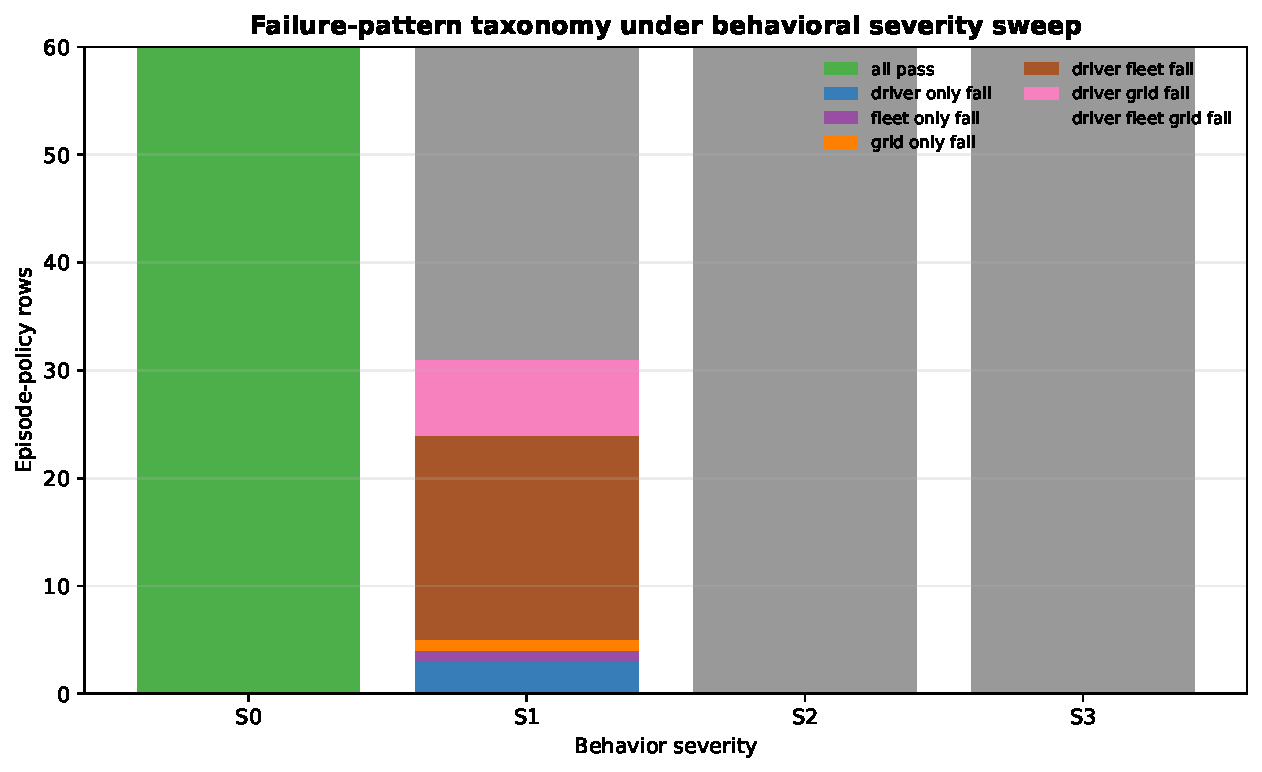
\includegraphics[width=0.9\textwidth]{figures/fig4_failure_pattern_taxonomy.pdf}
\caption{Failure-pattern taxonomy (Section~\ref{sec:results}). Most unacceptable cases fail multiple actor gates rather than a single isolated grid or service metric: across the weekly matrix, driver--operator--grid failure accounts for 209 of 300 rows.}
\label{fig:failure}
\end{figure}

\begin{figure}[H]
\centering
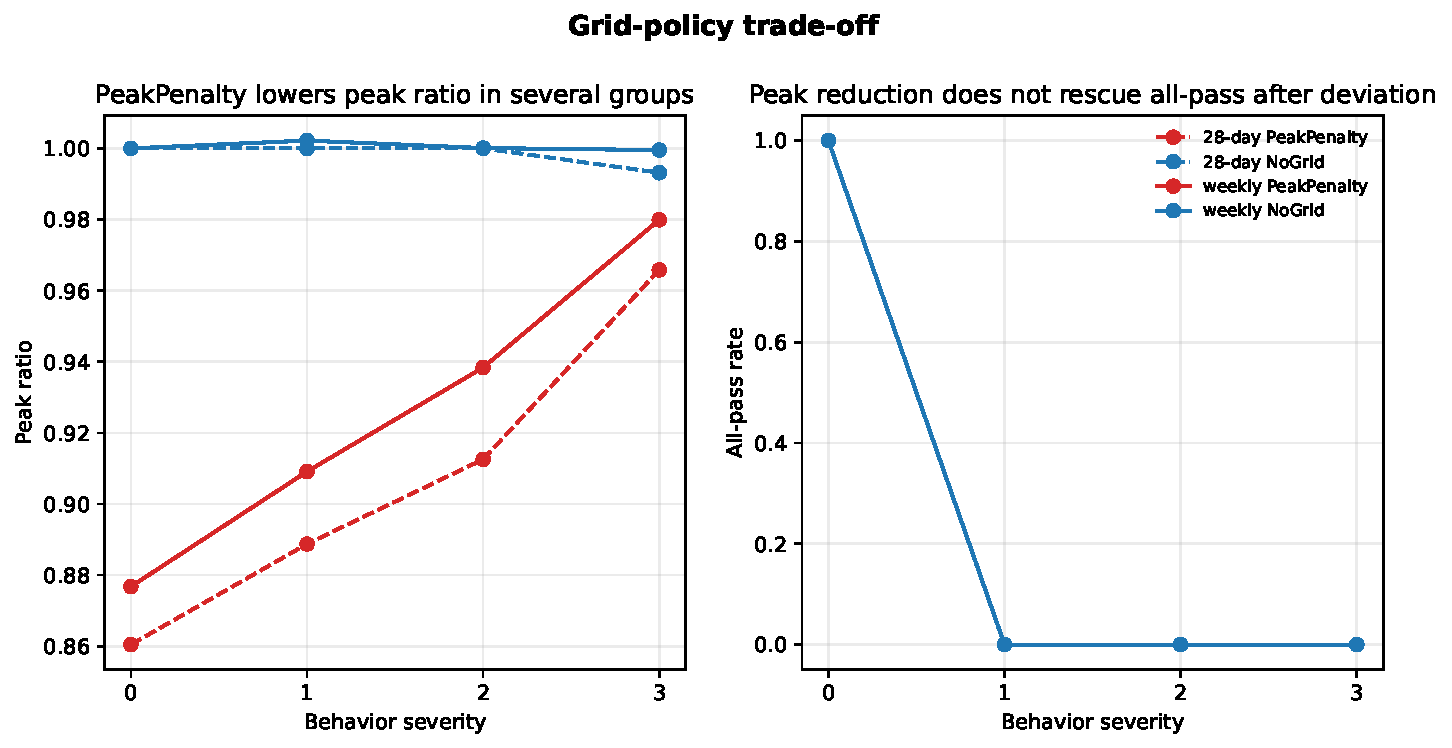
\includegraphics[width=0.9\textwidth]{figures/fig5_grid_policy_tradeoff.pdf}
\caption{Grid-policy trade-off (Section~\ref{sec:results}). PeakPenalty lowers selected peak metrics but does not rescue all-pass acceptability after driver and operator gates fail; the result is a bounded grid trade-off, not a rescue mechanism.}
\label{fig:gridtradeoff}
\end{figure}

\subsection*{Supplementary tables}

\paragraph{ServiceGridWeighted coefficient sensitivity ablation.} The six weight variants are: the base weights $320/175/120/95/55$ (with grid-penalty terms $48/32/18$); the normalized equivalents ($\div100$); equal service weights $100/100/100/100/100$; no grid penalty ($Q,P,R$ coefficients set to zero); and the base weights scaled by $\pm25\%$. Each was run at 35\% capacity for severities~0 and~1 across both grid policies and the five weekly seeds. Table~\ref{tab:sgwablation} reports the all-pass rates: every variant gives 1.00 under full compliance and 0.00 at severity~1, and the normalized variant reproduces the base weights' per-episode outcomes exactly, so the screening conclusion does not depend on the coefficient values. We restrict the ablation to severities~0 and~1 because these bracket the only non-trivial transition: all-pass is already $0.000$ for \emph{all} policies at severities~2 and~3 (Table~\ref{tab:weeklyseverity}), so no coefficient choice can lower it further, and coefficient-insensitivity at those higher severities is automatic. The $1.00\!\to\!0.00$ transition between severity~0 and~1 is therefore the discriminating case, and it is where we confirm the weights do not matter.

\begin{table}[H]
\centering
\caption{Supplementary: ServiceGridWeighted coefficient sensitivity ablation. All-pass rate at 35\% capacity, averaged over both grid policies and five seeds, for six weight variants.}
\label{tab:sgwablation}
\begin{tabular}{lcc}
\hline
Weight variant & All-pass, severity 0 & All-pass, severity 1 \\
\hline
Base ($320/175/120/95/55$) & 1.000 & 0.000 \\
Normalized ($\div 100$) & 1.000 & 0.000 \\
Equal service ($100$ each) & 1.000 & 0.000 \\
No grid penalty & 1.000 & 0.000 \\
Base $\times 1.25$ & 1.000 & 0.000 \\
Base $\times 0.75$ & 1.000 & 0.000 \\
\hline
\end{tabular}
\end{table}

\paragraph{ServiceGridWeighted scoring terms.} For request candidate $i$ at time $t$, the service score and, under an active queue/peak/price trigger, the deferral priority are
\begin{equation}
S_i = 320C_i + 175L_i + 120T_i + 95D_i + 55X_i,
\label{eq:sgwservice}
\end{equation}
\begin{equation}
Z_i = S_i - (48Q_i + 32P_t + 18R_t)F_i,
\label{eq:sgwpriority}
\end{equation}
where $C_i,L_i$ are critical-service and low-SoC indicators, $T_i,D_i$ are target- and deadline-energy deficits, $X_i$ is inverse laxity, $Q_i,P_t,R_t$ are queue, peak, and price pressure, and $F_i$ marks flexible low-risk status; at most $\lfloor 0.20 n_F \rfloor$ of the $n_F$ flexible low-risk candidates are deferred. Table~\ref{tab:sgwterms} lists the implemented scoring weights, term definitions, and code sources for reproducibility. The main argument depends only on the eligibility-based dominance described in Section~\ref{sec:formulation}, not on the exact coefficients.

\begin{table}[H]
\centering
\caption{Supplementary: implemented ServiceGridWeighted scoring and deferral terms.}
\label{tab:sgwterms}
\tiny
\begin{tabularx}{\textwidth}{p{0.12\textwidth}p{0.07\textwidth}Yp{0.12\textwidth}p{0.07\textwidth}p{0.09\textwidth}p{0.14\textwidth}}
\hline
Score term & Symbol & Definition & Normalization & Weight & Sign & Implementation source \\
\hline
Critical service & $C_i$ & reserve need OR deadline deficit $>0$ OR time-to-next mandatory $\leq 24/168$ OR laxity $\leq 0.25$ & binary & 320 & positive & service-grid rule; service-critical helper \\
Low SoC & $L_i$ & $SoC_i \leq \theta_i+0.05$ & binary & 175 & positive & service-grid weighted rule \\
Target deficit & $T_i$ & target-energy-deficit state & simulator normalized & 120 & positive & state-array helper \\
Deadline deficit & $D_i$ & deadline-energy-deficit state & simulator normalized & 95 & positive & state-array helper \\
Inverse laxity & $X_i$ & $1-\mathrm{clip}(deadline\ laxity,0,1)$ & [0,1] after clipping & 55 & positive & service-grid weighted rule \\
Queue pressure & $Q_i$ & $\max(0,(queued+requested-slots)/slots)$ at vehicle location & ratio & 48 & $-$ if flexible & queue-pressure helper \\
Projected peak pressure & $P_t$ & $\max(0,(n_{req}-0.85n_{slots})/n_{slots})$ & ratio & 32 & $-$ if flexible & service-grid rule \\
Price pressure & $R_t$ & current price divided by schedule maximum & ratio & 18 & $-$ if flexible & service-grid rule \\
Deferral cap & -- & defer lowest-priority flexible low-risk subset after trigger & 20\% of candidates; min. 1 & -- & remove action & service-grid rule \\
\hline
\end{tabularx}
\end{table}

\paragraph{Targeted 28-day confirmation.} Table~\ref{tab:target28} reports the targeted 28-day (672 h) behavioral severity confirmation at 35\% capacity (five seeds), discussed in Section~\ref{sec:results}; all-pass falls from 1.000 at severity~0 to 0.000 at severity~1, consistent with the weekly collapse.

\begin{table}[H]
\centering
\caption{Supplementary: targeted 28-day behavioral severity confirmation (35\% capacity, five seeds, 672 h horizon).}
\label{tab:target28}
\resizebox{\textwidth}{!}{%
\begin{tabular}{cccccccc}
\hline
Severity & Driver pass & Operator pass & Grid pass & All-pass & Actual/operator events & Delivered ratio & Peak ratio \\
\hline
0 & 1.000 & 1.000 & 1.000 & 1.000 & 0.995 & 1.000 & 0.930 \\
1 & 0.000 & 0.000 & 0.000 & 0.000 & 1.147 & 0.985 & 0.944 \\
2 & 0.000 & 0.000 & 0.000 & 0.000 & 1.625 & 0.954 & 0.956 \\
3 & 0.000 & 0.000 & 0.000 & 0.000 & 2.566 & 0.936 & 0.979 \\
\hline
\end{tabular}%
}
\end{table}

\paragraph{Threshold-slack robustness envelope.} Table~\ref{tab:envelope} reports acceptability under a global threshold-slack factor (all 14 gate margins scaled simultaneously), discussed in Section~\ref{sec:robust}; the severity-1 collapse persists until the whole gate system is loosened two- to threefold.

\begin{table}[H]
\centering
\caption{Supplementary: robustness envelope---acceptability under a global threshold-slack factor (all 14 gate margins scaled simultaneously; slack $>1$ loosens; 20-seed service-oriented family).}
\label{tab:envelope}
\begin{tabular}{ccccc}
\hline
Slack & All-pass sev 0 & All-pass sev 1 & Graded frac.\ sev 1 & $\geq$1 actor sev 1 \\
\hline
0.50 (tighter) & 0.912 & 0.000 & 0.725 & 0.246 \\
0.75 & 0.929 & 0.000 & 0.766 & 0.354 \\
1.00 (nominal) & 0.967 & 0.012 & 0.793 & 0.433 \\
1.25 & 0.992 & 0.046 & 0.827 & 0.567 \\
1.50 & 0.996 & 0.071 & 0.860 & 0.700 \\
2.00 & 0.996 & 0.458 & 0.947 & 1.000 \\
3.00 (looser) & 1.000 & 0.883 & 0.992 & 1.000 \\
\hline
\end{tabular}
\end{table}

\paragraph{Seed-resolved acceptability by capacity.} Table~\ref{tab:seedcap} resolves the all-pass rate by behavior severity and capacity (Section~\ref{sec:robust}): severity-0 acceptability declines and becomes more seed-variable as capacity rises, while the severity-1 collapse holds across all capacities.

\begin{table}[H]
\centering
\caption{Supplementary: seed-resolved all-pass acceptability by behavior severity and capacity (20 seeds, both grid policies, service-oriented family; each cell aggregates 80 episodes, standard deviation across the 20 per-seed all-pass means).}
\label{tab:seedcap}
\begin{tabular}{ccccc}
\hline
Severity & Capacity & All-pass mean & Seed std & Seed [min, max] \\
\hline
0 & 20\% & 0.988 & 0.056 & [0.75, 1.00] \\
0 & 35\% & 0.975 & 0.112 & [0.50, 1.00] \\
0 & 50\% & 0.938 & 0.160 & [0.50, 1.00] \\
1 & 20\% & 0.037 & 0.092 & [0.00, 0.25] \\
1 & 35\% & 0.000 & 0.000 & [0.00, 0.00] \\
1 & 50\% & 0.000 & 0.000 & [0.00, 0.00] \\
\hline
\end{tabular}
\end{table}

\paragraph{Welfare-weight sets in the price-of-anarchy sweep.} Table~\ref{tab:weights} lists the three welfare-weight vectors $(w_D,w_F,w_G)$ used in the game-parameter sweep of Section~\ref{sec:game} (one of the four sweep dimensions, alongside externality strength $\beta$, cost-heterogeneity scale $s$, and compliance anchor $\rho_0$). They are the three canonical normative stances bracketing the weight simplex---utilitarian, user-/adoption-centric, and system-operator---and the price of anarchy stays above one for all of them, so the welfare-gain conclusion does not depend on the choice of weights.

\begin{table}[H]
\centering
\caption{Supplementary: the three welfare-weight sets $(w_D,w_F,w_G)$ (driver, charging operator, grid) used in the price-of-anarchy sweep (Section~\ref{sec:game}). The same three sets are applied at each capacity. The actor utilities are min--max normalised within each capacity, so the weights combine comparable normalised utilities.}
\label{tab:weights}
\begin{tabular}{llccc}
\hline
Label & Normative stance & $w_D$ & $w_F$ & $w_G$ \\
\hline
Equal / utilitarian & no actor prioritized & $1/3$ & $1/3$ & $1/3$ \\
Driver-heavy & user-/adoption-centric & $0.50$ & $0.25$ & $0.25$ \\
Grid-heavy & system-operator & $0.25$ & $0.25$ & $0.50$ \\
\hline
\end{tabular}
\end{table}

\end{document}
